\documentclass[11pt]{scrartcl}
\usepackage[utf8]{inputenc}

% Packages
\usepackage[backend=biber,style=authoryear-icomp,sorting=ynt, doi=true]{biblatex}
%\usepackage[backend=biber,sorting=ynt]{biblatex}
\usepackage{hyperref}
\usepackage{graphicx}
%\usepackage[margin=1.25in]{geometry}
\usepackage{palatino}
\usepackage{mathpazo}
\usepackage{pgfplots}
\usepackage{amsmath}
\usepackage[hang]{subfigure}
\newcommand{\imagesource}[1]{{\footnotesize Source: #1}}
\usepackage[export]{adjustbox}[2011/08/13]
\usepackage{chngpage}
%\usepackage[dvipsnames]{xcolor}
\usepackage{titlesec}
\usepackage{listings} 
\setcounter{secnumdepth}{4}
\usepackage[section]{placeins} % Force images to belong to sections

% Metro
%\definecolor{custom_one}{HTML}{d11141}
%\definecolor{custom_two}{HTML}{00b159}
%\definecolor{custom_three}{HTML}{00aedb}
%\definecolor{custom_four}{HTML}{f37735}
%\definecolor{custom_five}{HTML}{ffc425}

%Eerie
%\definecolor{custom_one}{HTML}{11151c}
%\definecolor{custom_two}{HTML}{212d40}
%\definecolor{custom_three}{HTML}{364156}
%\definecolor{custom_four}{HTML}{7d4e57}
%\definecolor{custom_five}{HTML}{d66853}

%Viridis
\definecolor{viridis0}{rgb}{0.28, 0.13, 0.45}
\definecolor{viridis1}{rgb}{0.26, 0.24, 0.52}
\definecolor{viridis2}{rgb}{0.22, 0.34, 0.55}
\definecolor{viridis3}{rgb}{0.18, 0.44, 0.56}
\definecolor{viridis4}{rgb}{0.14, 0.52, 0.56}
\definecolor{viridis5}{rgb}{0.12, 0.61, 0.54}
\definecolor{viridis6}{rgb}{0.17, 0.69, 0.5}
\definecolor{viridis7}{rgb}{0.32, 0.77, 0.41}
\definecolor{viridis8}{rgb}{0.53, 0.83, 0.29}
\definecolor{viridis9}{rgb}{0.76, 0.88, 0.14}

%Catalogue
\definecolor{custom_one}{HTML}{00a0b0}
\definecolor{custom_two}{HTML}{eb6841}
\definecolor{custom_three}{HTML}{cc2a36}
\definecolor{custom_four}{HTML}{4f372d}
\definecolor{custom_five}{HTML}{183059}
\definecolor{custom_six}{HTML}{edc951}

% Argmax and Argmin
\DeclareMathOperator*{\argmax}{arg\,max}
\DeclareMathOperator*{\argmin}{arg\,min}

% Mathfont
%\usepackage{fontspec}
%\usepackage{unicode-math}
%\setmathfont{Stix Two Math}[version=stix2]

% Enable/Prettify the trace of a matrix
\DeclareMathOperator{\tr}{tr}

% Command needed for having a caption and source for pictures
\newcommand*{\captionsource}[2]{%
  \caption[{#1}]{%
    #1%
    \\\hspace{\linewidth}%
    \textbf{Source:} #2%
  }%
}

% Make texttt break
\renewcommand{\texttt}[1]{%
  \begingroup
  \ttfamily
  \begingroup\lccode`~=`/\lowercase{\endgroup\def~}{/\discretionary{}{}{}}%
  \begingroup\lccode`~=`[\lowercase{\endgroup\def~}{[\discretionary{}{}{}}%
  \begingroup\lccode`~=`.\lowercase{\endgroup\def~}{.\discretionary{}{}{}}%
  \catcode`/=\active\catcode`[=\active\catcode`.=\active
  \scantokens{#1\noexpand}%
  \endgroup
}

% Python Source Code
\usepackage{tcolorbox}
\tcbuselibrary{minted,breakable,xparse,skins}

\definecolor{bg}{gray}{0.95}
\DeclareTCBListing{mintedbox}{O{}mO{}}{%
  breakable=true,
  listing engine=minted,
  listing only,
  minted language=#2,
  minted style=default,
  minted options={%
    linenos,
    gobble=0,
    breaklines=true,
    breakafter=,,
    fontsize=\small,
    numbersep=8pt,
    #1},
  boxsep=0pt,
  left skip=0pt,
  right skip=0pt,
  left=25pt,
  right=0pt,
  top=3pt,
  bottom=3pt,
  arc=5pt,
  leftrule=0pt,
  rightrule=0pt,
  bottomrule=2pt,
  toprule=2pt,
  colback=bg,
  colframe=orange!70,
  enhanced,
  overlay={%
    \begin{tcbclipinterior}
    \fill[orange!20!white] (frame.south west) rectangle ([xshift=20pt]frame.north west);
    \end{tcbclipinterior}},
  #3}

% Line breaks for pasted code
\lstset{
	basicstyle=\ttfamily,
	columns=fullflexible,
	breaklines=true,
	postbreak=\mbox{\textcolor{viridis1}{$\hookrightarrow$}\space},
}

% Parameters
\hypersetup{
	citecolor={blue},
	linkcolor={red},
}

% Bib Settings
\addbibresource{literature.bib}

\title{Human Age Prediction Based on Real and Simulated RR Intervals using Temporal Convolutional Neural Networks and Gaussian Processes}
\subtitle{Division of Statistics and Machine Learning \\ Department of Computer and Information Science \\ Linköping University}
\subject{Master Thesis (732A64)}
\author{Maximilian Pfundstein (maxpf364)}
\date{\today}

\begin{document}

\pagenumbering{Roman}

\maketitle

\begin{center}
	\begin{tabular}{ll}
		Supervisor: & Krzysztof Bartoszek \\
		Examiner: & Oleg Sysoev \\
		\\
		ISRN: & LIU-IDA/STAT-A-\phantom{}-20/004-\phantom{}-SE 
	\end{tabular}
\end{center}

\begin{center}
	
\includegraphics{img/liu_primary_black_en.pdf}
\end{center}

%\bigskip

\newpage

\section*{Upphovsrätt}

Detta dokument hålls tillgängligt på Internet - eller dess framtida ersättare - under 23 år från publiceringsdatum under förutsättning att inga extraordinära omständigheter uppstår. Tillgång till dokumentet innebär tillstånd för var och en att läsa, ladda ner, skriva ut enstaka kopior för enskilt bruk och att använda det oförändrat för ickekommersiell forskning och för undervisning. Överföring av upphovsrätten vid en senare tidpunkt kan inte upphäva detta tillstånd. All annan användning av dokumentet kräver upphovsmannens medgivande. För att garantera äktheten, säkerheten och tillgängligheten finns lösningar av teknisk och administrativ art.

Upphovsmannens ideella rätt innefattar rätt att bli nämnd som upphovsman i den omfattning som god sed kräver vid användning av dokumentet på ovan beskrivna sätt samt skydd mot att dokumentet ändras eller presenteras i sådan form eller i sådant sammanhang som är kränkande för upphovsman	nens litterära eller konstnärliga anseende eller egenart.

För ytterligare information om Linköping University Electronic Press se förlagets hemsida \url{http://www.ep.liu.se/}.

\vspace*{\fill}

\section*{Copyright}

The publishers will keep this document online on the Internet - or its possible replacement - for a period of 25 years starting from the date of publication barring exceptional circumstances.

The online availability of the document implies permanent permission for anyone to read, to down- load, or to print out single copies for his/hers own use and to use it unchanged for non-commercial research and educational purpose. Subsequent transfers of copyright cannot revoke this permission. All other uses of the document are conditional upon the consent of the copyright owner. The publisher has taken technical and administrative measures to assure authenticity, security and accessibility. According to intellectual property law the author has the right to be mentioned when his/her work is accessed as described above and to be protected against infringement.

For additional information about the Linköping University Electronic Press and its procedures for publication and for assurance of document integrity, please refer to its www home page: \url{http://www.ep.liu.se/}.

\vspace*{\fill}

\clearpage

\section*{Abstract}

\begin{abstract}

Electrocardiography (ECG) is a non-invasive method used in medicine to track the electrical pulses sent by the heart. The time between two subsequent electrical impulses and hence the heartbeat of a subject, is referred to as an RR interval. Previous studies show that RR intervals can be used for identifying sleep patterns and cardiovascular diseases. Additional research indicates that RR intervals can be used to predict the cardiovascular age of a subject. This thesis investigates, if this assumption is true, based on two different datasets as well as simulated data based on Gaussian Processes. The datasets used are Holter recordings provided by the University of Gdańsk as well as a dataset provided by Physionet. The former represents a balanced dataset of recordings during nocturnal sleep of healthy subjects whereas the latter one describes an imbalanced dataset of records of a whole day of subjects that suffered from myocardial infarction. Feature-based models as well as a deep learning architecture called DeepSleep, based on a paper for sleep stage detection, are trained. The results show, that the prediction of a subject's age, only based in RR intervals, is difficult. For the first dataset, the highest obtained test accuracy is 37.84 per cent, with a baseline of 18.23 per cent. For the second dataset, the highest obtained accuracy is 42.58 per cent with a baseline of 39.14 per cent. Furthermore, data is simulated by fitting Gaussian Processes to the first dataset and following a Bayesian approach by assuming a distribution for all hyperparameters of the kernel function in use. The distributions for the hyperparameters are continuously updated by fitting a Gaussian Process to a slices of around 2.5 minutes. Then, samples from the fitted Gaussian Process are taken as simulated data, handling impurity and padding. The results show that the highest accuracy achieved is 31.12 per cent with a baseline of 18.23 per cent. Concludingly, cardiovascular age prediction based on RR intervals is a difficult problem and complex handling of impurity does not necessarily improve the results.

\end{abstract}

\clearpage

\vspace*{\fill}

\section*{Acknowledgements}

I want to thank my supervisor Krzysztof Bartoszek for continuously supporting me throughout the writing of this thesis. Also, I want to say thank you to Anna and Julia for proofreading and giving advice.

\vspace*{\fill}

\clearpage

\vspace*{\fill}

\section*{Preamble}

This thesis, the source code and all conducted analysis can be found on GitHub at \url{https://github.com/flennic/master-thesis/}.

In some occasions throughout the thesis, a function is used on a matrix. This is mostly the case for activation functions being applied to a linear combination embedded into a matrix. To keep the notation short, the indexes are omitted. Mathematically, the activation function is applied on each linear combination of the feature vector and the weights of the model.

\vspace*{\fill}

\clearpage

\tableofcontents

\clearpage

\null
\vspace*{\fill}

\begin{figure}[hbt]
	\center
	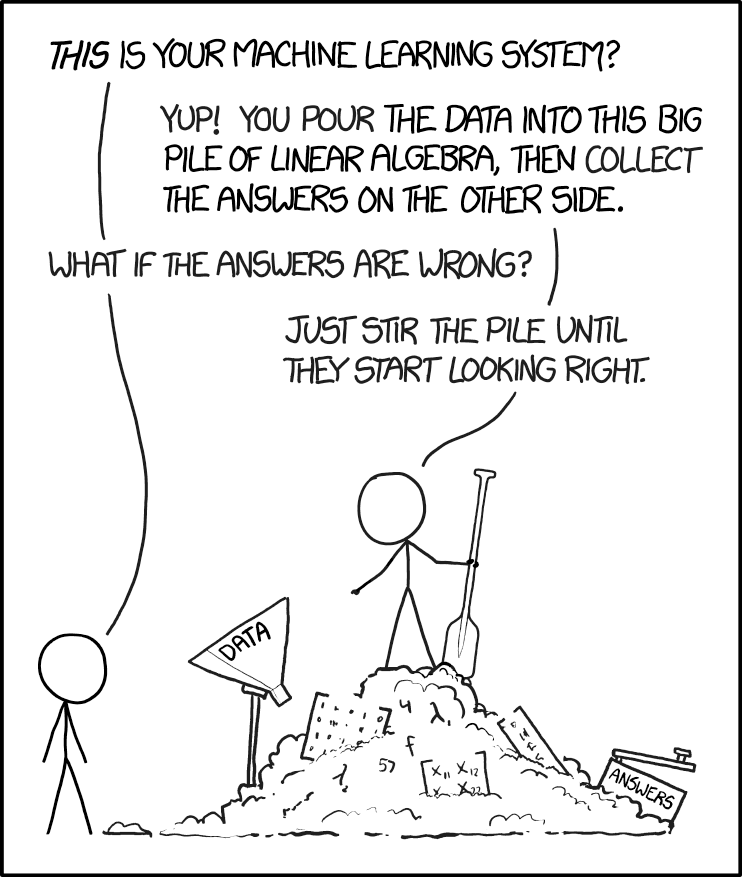
\includegraphics[width=0.8\textwidth]{img/machine_learning_2x.png}
	\caption{By Randall Munroe. \textit{Source:} \texttt{https://xkcd.com/1838/}}
	\label{fig:xkcd_machine_learning}
\end{figure}

\vspace*{\fill}

\clearpage
\pagenumbering{arabic}
\section{Introduction}

\subsection{Background}

In the field of medicine, electrocardiography (ECG) is a procedure of measuring the electrical potential and thereby the voltage between different potential levels of the heart. These measurements can be used to monitor the electrical activity of the heart which are fundamentally responsible for heart contractions and the heart rhythm. The analysis of these impulses can be used to study the health of a patient in a non-invasive way, inferentially ECG is used amongst other methods for detecting and analysing cardiovascular diseases [\cite{doi:10.1161/CIRCOUTCOMES.118.005289}], myocardial infarction [\cite{FESMIRE1988405}] or acute coronary syndromes [\cite{doi:10.1111/anec.12196}]. An example of such a measurement can be seen in figure \ref{fig:rr_interval}. The data displayed is a signal used for testing\footnote{\url{https://physionet.org/content/aami-ec13/1.0.0/\#files-panel}} ECG devices and was obtained using the \textit{WFDB Software Package}\footnote{\url{https://archive.physionet.org/physiotools/wfdb.shtml}}, issuing the command \texttt{rdsamp -r aami3a -p > out.txt} and then slicing the values between indices $10000$ and $12000$. The signal was recorded using a sampling rate of $720 \text{Hz}$ and a resolution of $12$ bit. Figure \ref{fig:rr_interval} thereby shows the period of $2.78$ seconds including two RR spikes, thus one RR interval. The QRS complex can be seen as well, having a lower voltage before (Q) and after (S) the R spike. The remaining indices are used in the field of medicine, but are not considered for this thesis, as the data of interest consists of only RR intervals.

\begin{figure}[hbt]
	\center
	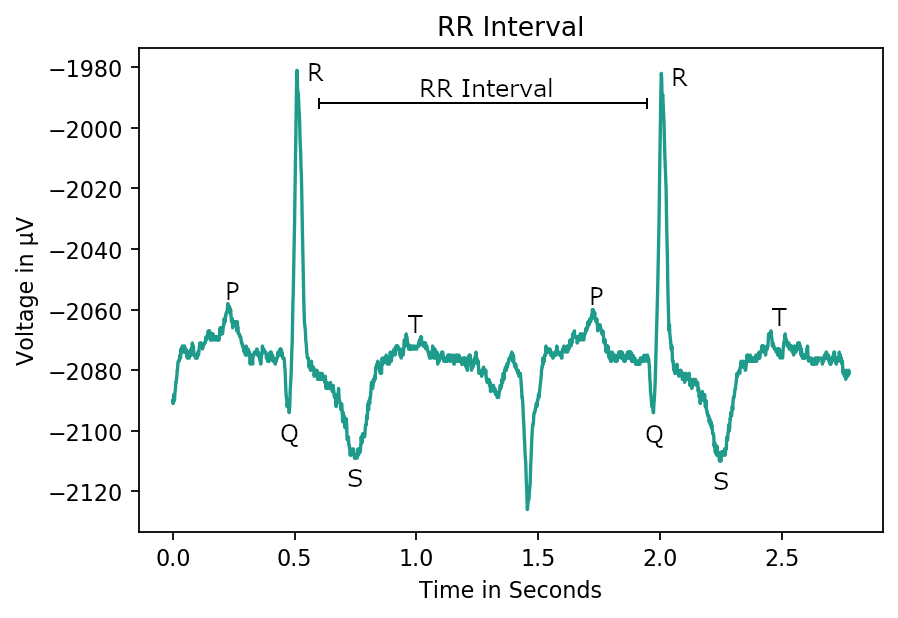
\includegraphics[width=1.0\textwidth]{img/general/rr-interval.png}
	\caption{\textcolor{viridis5}{\textbf{Sinus Rhythm}} with labels.}
	\label{fig:rr_interval}
\end{figure}

Earlier studies analysed the correlation between different features of RR signals and the age of the subject [\cite{patternshrd}] or focus on sleep stage classification using deep learning [\cite{sleepstageclassification}]. This thesis will emphasise on the prediction of the age of a subject given the RR intervals. The interest of this task is two-fold: Firstly, it seems that the process of collecting and archiving data is not always standardised, resulting in inconsistently formatted data, especially unlabelled RR intervals in the field of medicine. These labels are a necessity for researching this domain [e.g. \cite{10.3389/fphys.2018.00424}], therefore, the prediction of age with a high accuracy is of importance. Secondly, having a model available that predicts the age of healthy humans can be useful for estimating the cardiovascular age of unhealthy individuals. Assuming that the actual age and cardiovascular age of a healthy individual is the same, the model can be used to estimate the cardiovascular age of an unhealthy individual, as the cardiovascular age can be higher compared to the actual age, especially if the individual, for example, smokes.

[\cite{patternshrd}] focus on constructing and analysing $33$ features from a given RR interval time series, used for traditional machine learning models like Support Vector Machines (SVMs). These features are well known in the analysis of RR intervals [\cite{features_well_known}], some of them being correlated though and thereby do not add too much information for a feature-based classifier. Each subject's age decade (e.g. from 20 to 29) resembles one class, yielding in 7 classes (20-29, 30-39, 40-49, 50-59, 60-69, 70-79, 70+) for the dataset used\footnote{Which is also one of the datasets used in this thesis, provided by the University of Gdańsk.}. The paper reports very high accuracies for this task of age classification. An accuracy of $94$ per cent for a non-linear SVM using all features and an accuracy of $98$ per cent using a majority vote for the classification of 5 minutes chunks using only \textit{minimal stdRR} and \textit{minimal HR} [\cite{patternshrd}, p. 16 and 17] as features.

These accuracies seem to be very high, considering the only validation which is being conducted was to shuffle the time signal and comparing a model trained on the shuffled data, which results in lower accuracies. By this, according to the paper, the distribution of values is preserved, but the order of the time series is destroyed. This is supposed to be sufficient for validating the obtained results. The absence of an actual validation or test set raises the question, if the classifiers learned to generalise or whether they overfitted the data that is used for training and prediction. They also state: \textit{One can see that restriction of the set of features limited the classification quality, namely the score was significantly smaller than in the case when all features were taken into account} [\cite{patternshrd}, p. 16]. This seems to be another indicator that the trained classifiers might be overfitted, as more features can lead to an overfit.

Another study [\cite{threeclassclassification}] also tries to classify subjects by age, based on given RR intervals. They also utilise feature-based classifiers and define three classes:

\begin{itemize}
    \item \textbf{Y}oung (18-30)
    \item \textbf{M}iddle (30-45)
    \item \textbf{O}ld (45-60)
\end{itemize}

A test set was used in this analysis [\cite{threeclassclassification}, p. 4] and the results show an accuracy of around $70$ per cent. This lower accuracy is contrary compared to having fewer classes ($3$ instead of $7$), further raising the question, if the previous high accuracies might be the result of an overfit to the training data. Additionally, the reported classes in [\cite{threeclassclassification}] seem to overlap, at least the way they are defined in the paper. Both papers do not consider the order of classes. The order might allow conclusions about how much a prediction is off from the real class label as it makes a considerable difference if a subject of 20 years of age was misclassified as 30 or 70. The way the accuracies and thus the models are presented in both papers, automatically yield in a higher accuracy the less classes are defined. The actual predictive power of a model in terms of general predictability (e.g. regression) does not depend on the number of classes, but rather on prediction intervals and the respective error distributions. Of course, for the downstream task of classification, such an accuracy as a metric can be reported, but it makes the models incomparable. Furthermore, it seems that both analysis lack a real baseline model, hence they do not account for probable inequality in class distributions or the mentioned fact that the classes are ordered. More precisely, they do not state the loss function used, as e.g. cross-entropy loss does not account for the order of classes.

The domain of deep learning provides tools for time series prediction as well, namely Long Short-Term Memories (LSTMs) as they do not suffer that much from the vanishing gradient problem [\cite{10.1162/neco.1997.9.8.1735}, abstract] compared to traditional Recurrent Neural Networks (RNNs) [\cite{pascanu2012difficulty}] or Convolutional Neural Networks (CNN). CNNs use convolutions and thus moving averages in the discrete case [\cite{dlclassification}, p. 7]). [\cite{dlclassification}] researched time series classification, specifically looking into Time Convolutional Neural Networks (TCNNs) which were first proposed by [\cite{tcnn}]. The main difference to traditional CNNs is that instead of a cross-entropy loss the mean squared error (MSE) is being taken and that instead of \textit{max} pooling, \textit{average} pooling is being used [\cite{dlclassification}]. Therefore, this thesis will also investigate, how well deep learning models work for this task of age classification compared to traditional feature-based models.

\subsection{Objectives and Research Questions}

The main research question this thesis aims to answer:

\begin{itemize}
    \item Can the (cardiovascular) age of a person be predicted using recorded RR intervals and if yes, to which extend?
    \item Can RR intervals be simulated to generate training data, especially for deep learning models? How well does this work and does it improve the accuracy of the models?
\end{itemize}

For answering these research question, the following steps are conducted:

\begin{itemize}
	\item Use feature-based models and investigate to which extend the previous results can be replicated.
	\item Building a deep learning to analyse if this approach works better compared to feature-based models.
	\item Find a better way of handling the impurity of the data by creating a statistical model for the data.
	\item Use the obtained statistical model to simulate training data for the deep learning model to increase the variability of the data and examine if that increases the predictive strength of both kinds of models.
\end{itemize}

A more detailed overview of the different models and planned approaches is given in section \ref{sec:roadmap}. The following chapter will present the two datasets used in this thesis.

\clearpage
\section{Data}

The objective of age prediction is carried out on two datasets. For data simulation, only the first dataset, provided by the University of Gdańsk, will be used.

\subsection{Holter Recordings from the University of Gdańsk}

 The first dataset was acquired during the analysis of \textit{gdaHeart Rate Dynamics in Healthy Aging Population: Insights from Machine Learning Methods} [\cite{patternshrd}] and consists of $181$ Holter recordings of healthy individuals. For each individual, gender, age decade and beginning of the recording are available as meta-information. An age decade, which is for example denoted by $20$, means that the subject's age lies between $20$ and $29$ years. The distribution of age decades, number of classes and respective amounts of males and females are displayed in figure \ref{fig:gdansk-distribution-subjects}. The dataset is not completely balanced, still the amount of samples from each class label lies within a factor of two.

\begin{figure}[hbt]
    \makebox[\linewidth][c]{
	\centering
	\subfigure[Distribution of Individuals]{\label{fig:gdansk-distribution-subjects}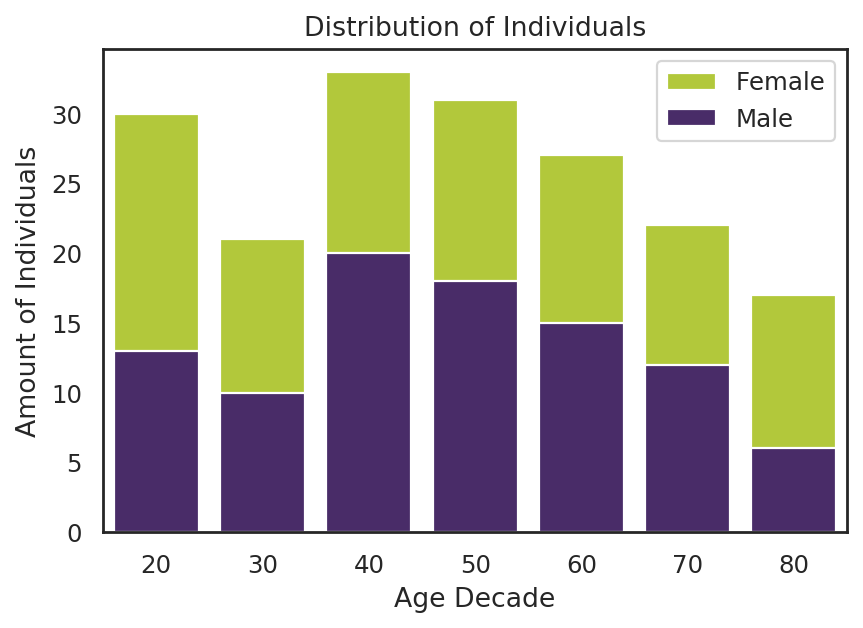
\includegraphics[width=0.6\textwidth]{img/data/gdansk-distribution-subjects.png}}
	\subfigure[Distribution of Recording Lengths ]{\label{fig:gdansk-distribution-recordings}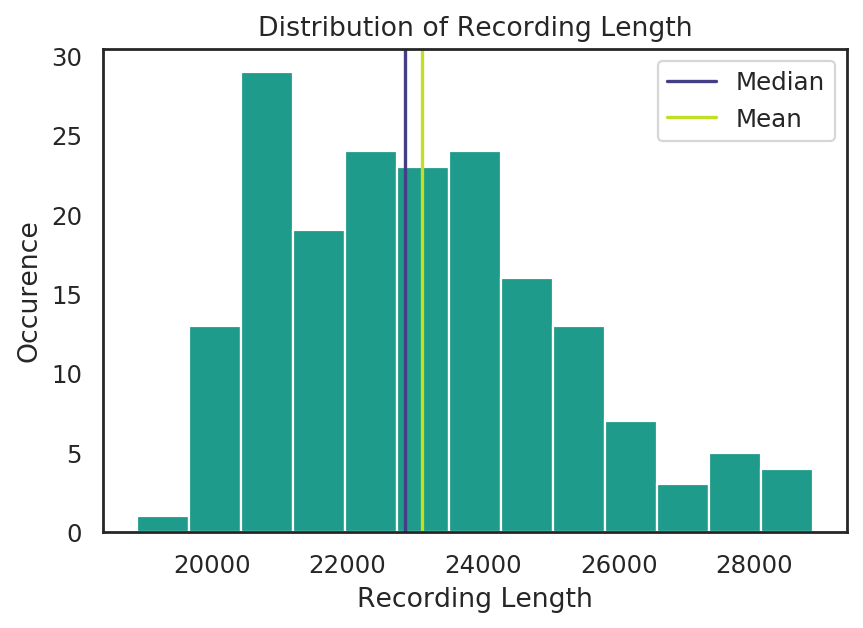
\includegraphics[width=0.6\textwidth]{img/data/gdansk-distribution-recording-lengths.png}}
	}
	\caption{Distribution of individuals, split by \textcolor{viridis0}{\textbf{male}} and \textcolor{viridis9}{\textbf{female}}, and \textcolor{viridis5}{\textbf{recording lengths}} (Gdańsk) with \textcolor{viridis9}{\textbf{mean}} and \textcolor{viridis0}{\textbf{median}}.}
\end{figure}

The dataset is provided by the \textit{Institute of Theoretical Physics and Astrophysics, University of Gdańsk} and is already preprocessed to some degree. Firstly, the recordings include only the RR intervals and no further information like the QRS-complex are available. Secondly, the dataset has been truncated to only include the first four hours of nocturnal sleep for each subject. This process was conducted by manual inspection of the signal. In the case the beginning of an individual's sleep was not evident, the signal starts at 00:00. Thirdly, gaps of size $1$ and $2$ were filled by the median value of the adjacent signals and each $\delta RR$ was capped to $\pm 300\text{ms}$ [\cite{patternshrd}, p.4].

The distribution of the recording's lengths with its mean and median can be seen in figure \ref{fig:gdansk-distribution-recordings}. The $95$th percentile of the recording's lengths lies at $26959$.

\begin{figure}[hbt]
    \makebox[\linewidth][c]{
	\centering
	\subfigure[Amount of Gaps for each Series]{\label{fig:gdansk-amount-of-gaps-per-series}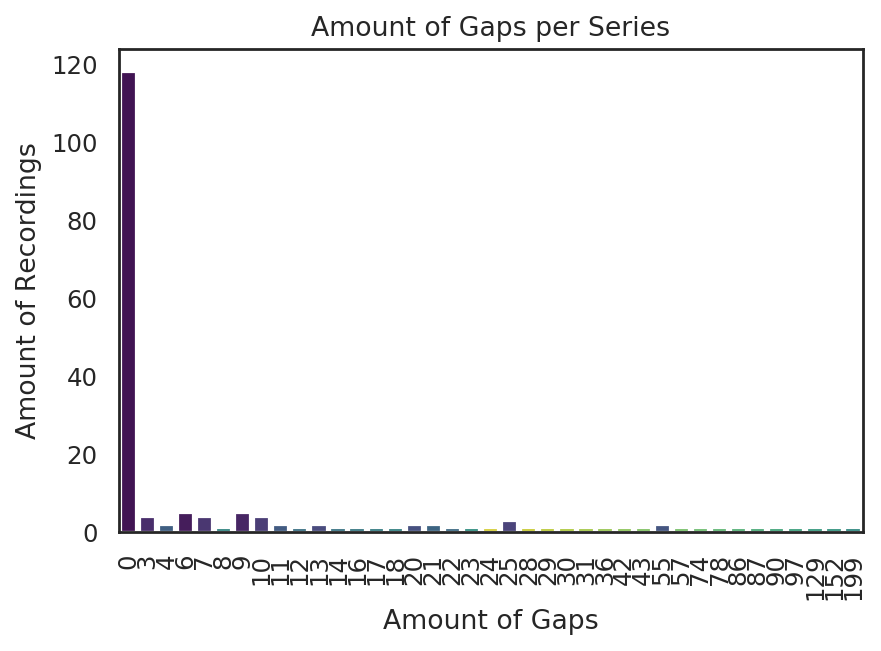
\includegraphics[width=0.6\textwidth]{img/data/gdansk-amount-of-gaps-per-series.png}}
	\subfigure[Logged Amount of Gaps ]{\label{fig:gdansk-overall-lengths-of-gaps}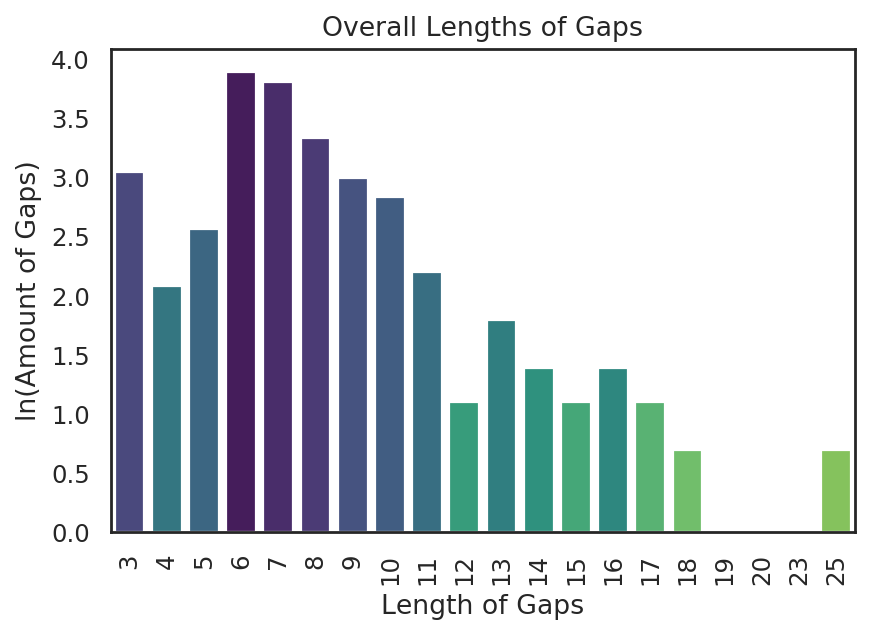
\includegraphics[width=0.6\textwidth]{img/data/gdansk-overall-lengths-of-gaps.png}}
	}
	\caption{Distribution of amount of gaps and length of gaps (Gdańsk).}
\end{figure}

Figure \ref{fig:gdansk-amount-of-gaps-per-series} shows that approximately 60 per cent of the series do not contain any gaps. For the remaining series, the distribution of the gap's lengths can be seen in figure \ref{fig:gdansk-overall-lengths-of-gaps}. In the following, this dataset will be referred to as the \textit{Gdańsk dataset}.

\subsection{CAST RR Interval Sub-Study Database}

The second dataset is available at PhysioNet [\cite{physionet}] and is called \textit{CAST RR Interval Sub-Study Database}. It consists of $1543$ recordings of individuals that survived a myocardial infarction. Each subject was treated with a different medication: $285$ with \textit{Encainide}, $229$ with  \textit{Flecainide} and $294$ with \textit{Moricizine}. Recordings before the treatment are available for most subjects, explaining the overall amount of recordings. For each subject, full 24 hours of recording are available compared to the first dataset, which provides only 4 hours of nocturnal sleep. The purpose of using this additional dataset is to ascertain that the obtained generalised predictabilities of the models also hold roughly for another dataset as well as analysing different methods of handling imbalance in the data. In theory, a vast amount of data from different sources is ideal, but the acquisition and amount of computational resources are out of scope for this thesis. One must be aware that models trained on this second dataset might be biased, as RR intervals with diseases are not labelled according to the subjects cardiovascular, but real age. As this thesis focuses mainly on the question if any information about the age can be extracted from the RR intervals in the first place, this bias does not pose a problem.

\begin{figure}[hbt]
    \makebox[\linewidth][c]{
	\centering
	\subfigure[Distribution of Individuals]{\label{fig:physionet-distribution-subjects}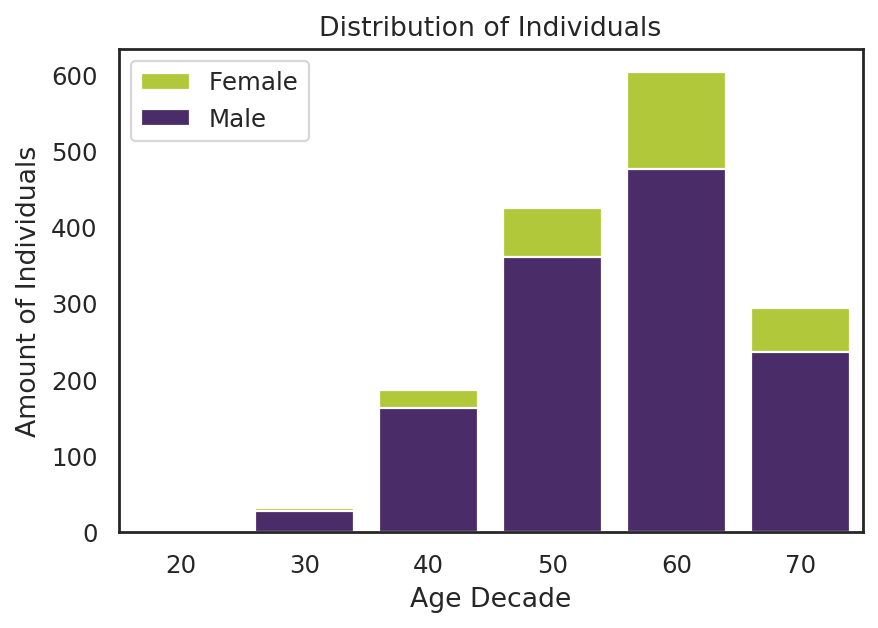
\includegraphics[width=0.6\textwidth]{img/data/physionet-distribution-subjects.png}}
	\subfigure[Distribution of Recording Lengths]{\label{fig:physionet-distribution-recordings}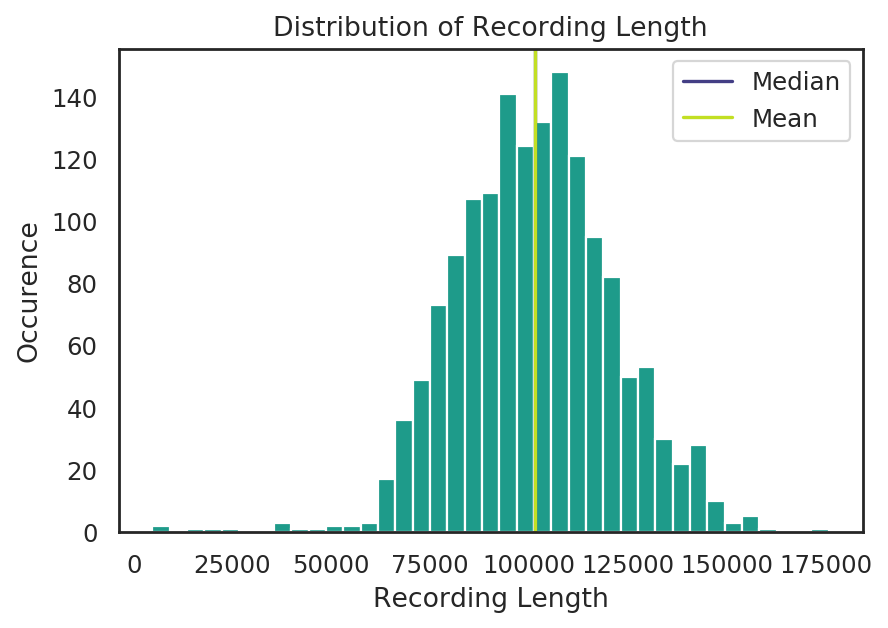
\includegraphics[width=0.6\textwidth]{img/data/physionet-distribution-recording-lengths.png}}
	}
	\caption{Distribution of individuals, split by \textcolor{viridis0}{\textbf{male}} and \textcolor{viridis9}{\textbf{female}}, and \textcolor{viridis5}{\textbf{recording lengths}} (PhysioNet) with \textcolor{viridis9}{\textbf{mean}} and \textcolor{viridis0}{\textbf{median}}, which are covering each other due to their closeness.}
\end{figure}

For this second dataset, the distribution of age decades is shown in figure \ref{fig:physionet-distribution-subjects}. It reveals that this dataset is more imbalanced compared to the first one. There are only $2$ individuals for the age decade $20-29$, also males are more represented compared to females. As the dataset contains recordings for the whole day, the length of each series is around six times longer. The distribution, the respective mean and median, which are almost the same for this dataset, can be seen in figure \ref{fig:physionet-distribution-recordings}.

The RR intervals are extracted from the raw data recordings using the \textit{WFDB Software Package}\footnote{\url{https://archive.physionet.org/physiotools/wfdb.shtml}}. The obtained signals contain outliers and therefore are preprocessed using the Python package \texttt{hrvanalysis}\footnote{\url{https://github.com/Aura-healthcare/hrvanalysis}} with its function \texttt{hrvanalysis.preprocessing.remove\_outliers(...)}, based on the following previous studies: [\cite{cardiopulmonary}], [\cite{maxhr}], [\cite{TANAKA2001153}] and [\cite{doi:10.1161/CIRCULATIONAHA.110.939249}]. Outliers will be treated as missing data points.

\begin{figure}[hbt]
    \makebox[\linewidth][c]{
	\centering
	\subfigure[Amount of Gaps for each Series (first 20)]{\label{fig:physionet-amount-of-gaps-per-series}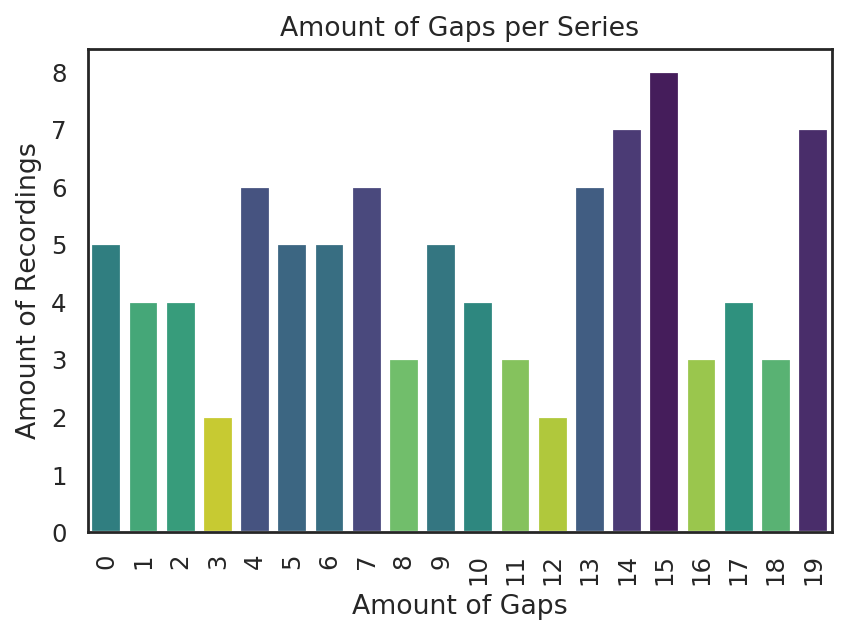
\includegraphics[width=0.6\textwidth]{img/data/physionet-amount-of-gaps-per-series-head.png}}
	\subfigure[Logged Amount of Gaps ]{\label{fig:physionet-overall-lengths-of-gaps}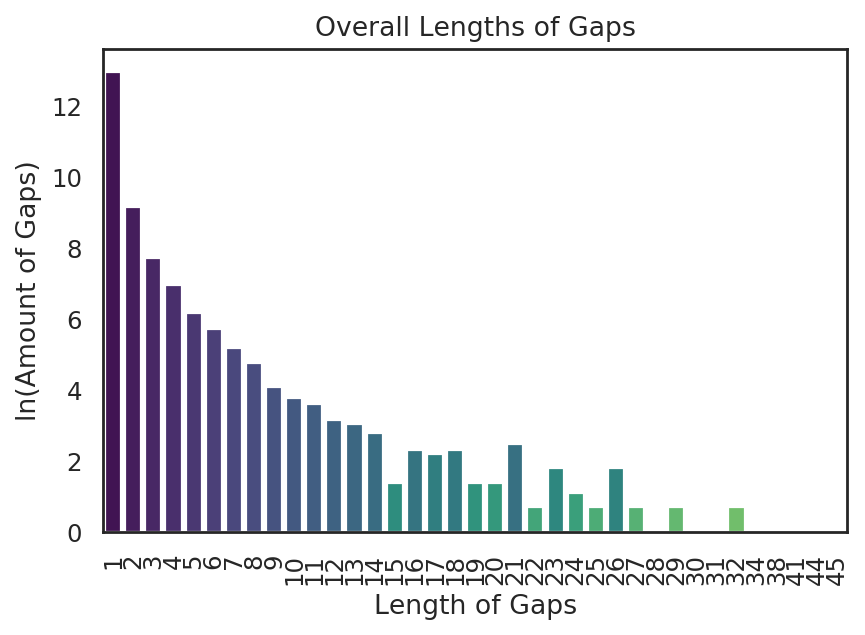
\includegraphics[width=0.6\textwidth]{img/data/physionet-overall-lengths-of-gaps.png}}
	}
	\caption{Distribution of amount of gaps and length of gaps (PhysioNet).}
\end{figure}

Figure \ref{fig:physionet-amount-of-gaps-per-series} shows the ordered amount of gaps per series capped at a length of 20. This dataset includes some very large gaps, excelling at $4437$ missing data points in a row. For preprocessing, these large gaps provide a challenge, as simple spline interpolations might not result in an appropriate fit, especially when considering the trigonometric behaviour of the signals. Figure \ref{fig:gdansk-example-100-head} and figure \ref{fig:gdansk-example-100-tail} show an excerpt of the overall time series of a young, healthy male. Figure \ref{fig:gdansk-example-100-head} illustrates, that in the beginning of the recording, the subject's sleep phase started, yielding in slower heart contractions and thus larger RR intervals. The interval itself indicates the trigonometric pattern, which is more evident in figure \ref{fig:gdansk-example-100-tail} and shows the RR intervals during the end of the sleep phase.

\begin{figure}[hbt]
    \makebox[\linewidth][c]{
	\centering
	\subfigure[First 100 RR intervals for a young, healthy male]{\label{fig:gdansk-example-100-head}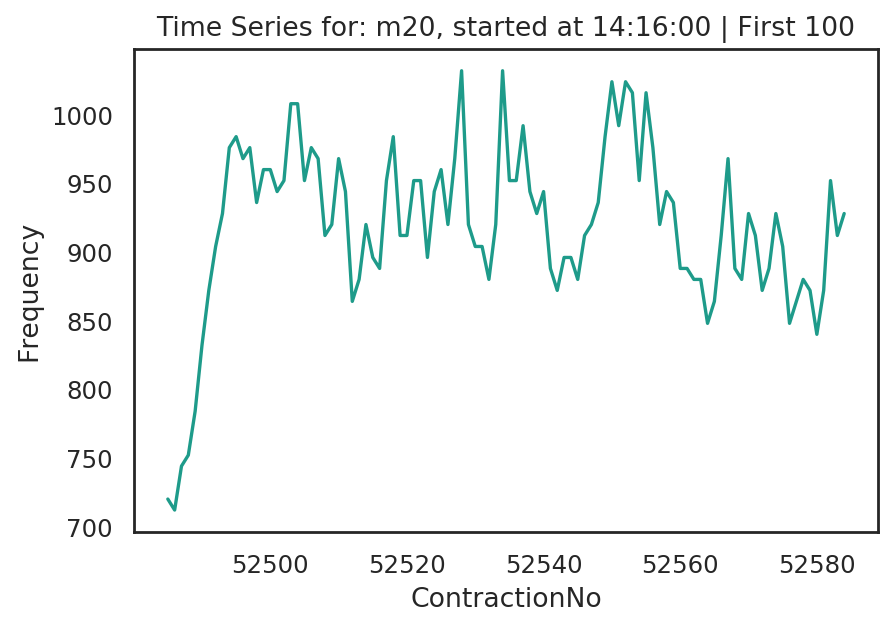
\includegraphics[width=0.6\textwidth]{img/data/gdansk-example-100-head.png}}
	\subfigure[Last 100 RR intervals for a young, healthy male]{\label{fig:gdansk-example-100-tail}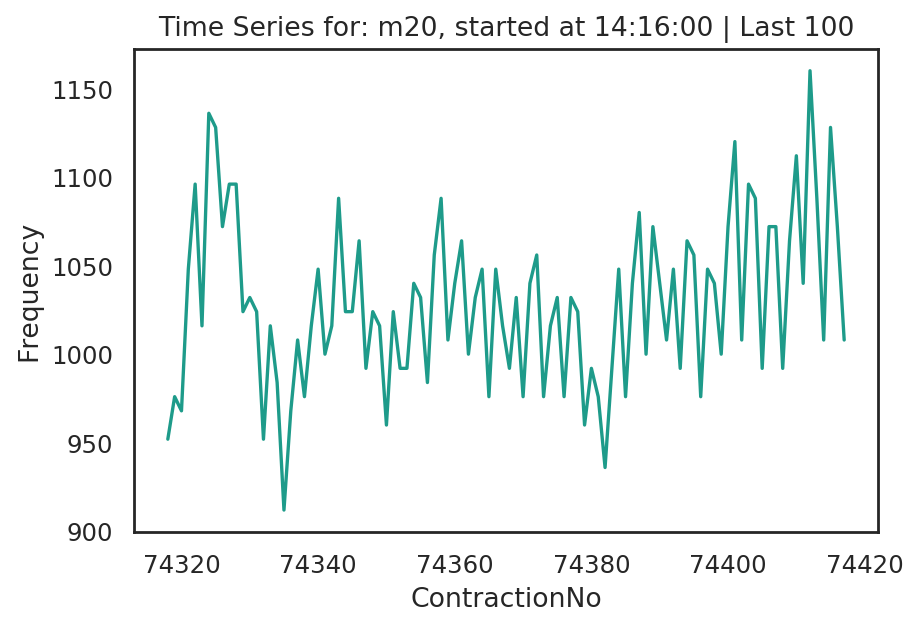
\includegraphics[width=0.6\textwidth]{img/data/gdansk-example-100-tail.png}}
	}
	\caption{Example excerpt from the time series, showing the \textcolor{viridis5}{\textbf{first and last 100 RR intervals}} of the series of a healthy, young male.}
\end{figure}

Looking at an older female, who is a survivor of a myocardial infarction, shown in figure \ref{fig:physionet-example-100-head}, it can be seen that firstly, there are two spikes which seem out of the ordinary and secondly, that the trigonometric pattern is not as evident. Moreover, in figure \ref{fig:physionet-example-100-tail} the mean of the series seems to change with time, whereas compared to \ref{fig:gdansk-example-100-tail} the mean seems more steady. The female subject might still have been awake during the end of the recording and is under the influence of medication, so the comparison might not provide too much information. Still, it seems that there is a difference between RR intervals of different subjects that can be investigated for predicting the age. This dataset will be referred to as the \textit{Physionet dataset}.

\begin{figure}[hbt]
    \makebox[\linewidth][c]{
	\centering
	\subfigure[First 100 RR intervals for an older female]{\label{fig:physionet-example-100-head}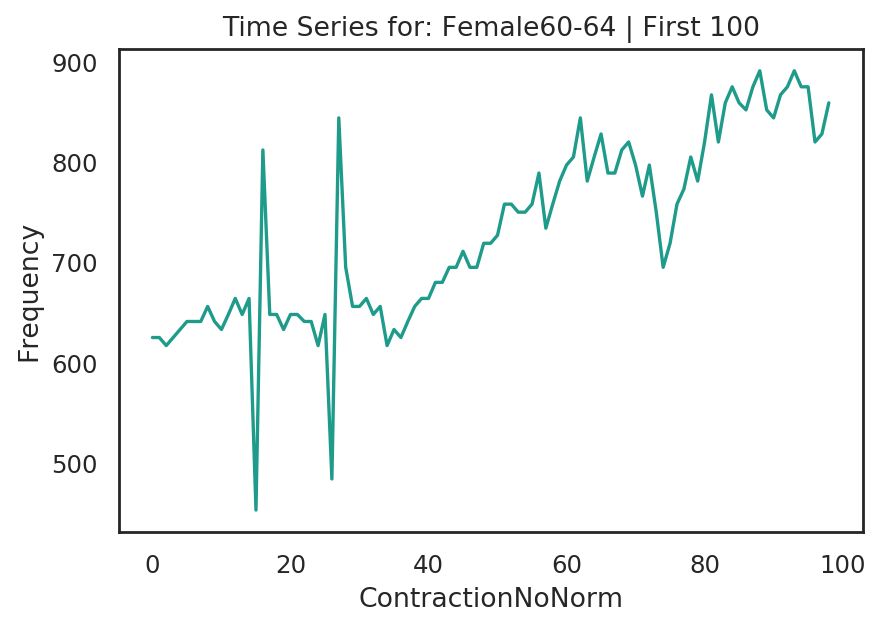
\includegraphics[width=0.6\textwidth]{img/data/physionet-example-100-head.png}}
	\subfigure[First 100 RR intervals for an older female]{\label{fig:physionet-example-100-tail}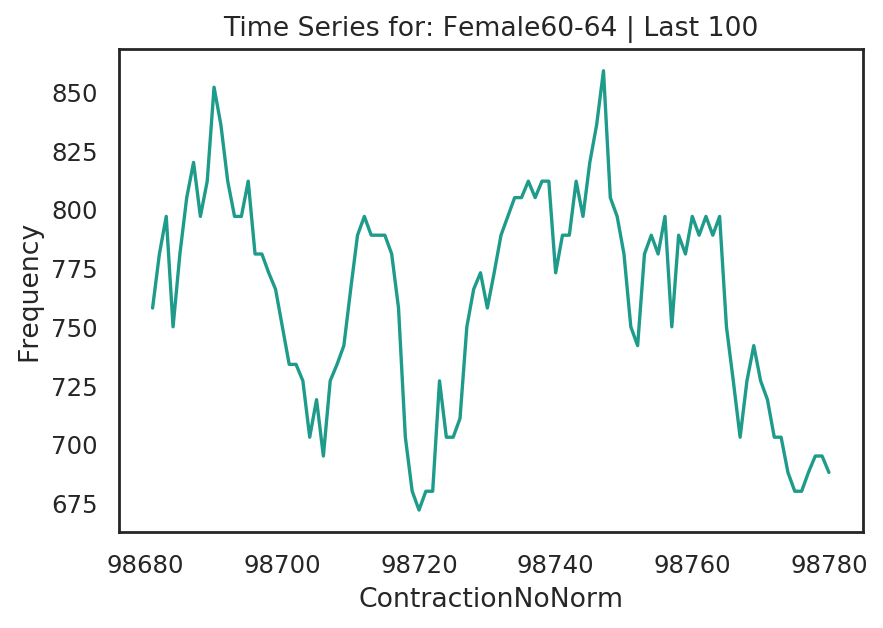
\includegraphics[width=0.6\textwidth]{img/data/physionet-example-100-tail.png}}
	}
	\caption{Example excerpt from the time series, showing the \textcolor{viridis5}{\textbf{first and last 100 RR intervals}} of the series of an older female, who is a survivor of a myocardial infarction and under treatment of medication.}
\end{figure}


\clearpage
\section{Theory}

This chapter explains the different theoretical frameworks used in this thesis for answering the defined research questions. Firstly, a roadmap and thus an overview of the models is given. Secondly, the feature-based models and their choice of hyperparameters will be presented. Thirdly, the focus will shift towards deep learning and the modified version of a model proposed by another paper for a similar task is being analysed. Afterwards, different approaches for handling impurity and padding of the data are described, which includes interpolation (linear splines) and data simulation by using $\mathcal{GP}s$.

\subsection{Roadmap}
\label{sec:roadmap}

To answer the research questions, the first aim is to rebuild the SVM baseline model based the $33$ features used in previous studies and to use cross-validation and hyperparameter search to understand the previous findings of [\cite{patternshrd}]. Afterwards, a more precise accuracy estimate is obtained by using a test set as well. Additionally, the following feature-based methods will be trained as well to investigate how well these models generalise: \textit{XGBoost}, \textit{Random Forests} and \textit{Naive Bayes}.

For applying a deep learning approach, a model based on DeepSleep, proposed by [\cite{deepsleep}], will be trained. It consists of two CNNs heads, followed by an LSTM and a Multi-Layer Perceptron (MLP) for the downstream task of classification. It will be adjusted according to [\cite{dlclassification}], which includes changing the pooling layer as well as the the loss function. Further reasons and explanations that led to choosing this model are explained in the theory chapter.

All models, feature-based and DeepSleep, will be trained and tested for classification and regression, whereas classification assumes no order of the classes and regression does. In the case of regression, the median of the age decade will be taken (e.g. 30-39 will result in 35). Also, two types of slicing will be applied to the data:

\begin{itemize}
    \item \textbf{Complete} (the whole time series is being taken)
    \item \textbf{Constant} (the time series is split into equal chunks resembling a time frame of around 5 minutes)
\end{itemize}

For replicating the results by [\cite{patternshrd}] and to compare them to other feature-based models, spline interpolation will be used.

The second aim is two-folded: Firstly, the impurity of the data should be handled using a more sophisticated approach. Secondly, training data should be simulated to have more variability in the data, leading to less overfit, which is especially useful for the DeepSleep-based model. Gaussian Processes ($\mathcal{GP}s$) are particularly valuable in this scenario of time series modelling as they cover both aims [\cite{Roberts_gaussianprocesses}]. Firstly, $\mathcal{GP}s$ are defined as a distribution over functions, which means that the fitted $\mathcal{GP}$ can be evaluated at all desired predictive index points. This enables evaluating predictive index points which were originally not included in the observations. Therefore, missing data points, as well as parts of the series that need to be padded for the DeepSleep model, are covered. Secondly, as we have a distribution over functions, any amount of samples can be taken, providing a larger amount of training data. Thirdly, a posterior distribution is being provided which can subsequently be used for sampling differently shaped time series for training.

This will be done by fitting $\mathcal{GP}s$ to each slice of around 5 minutes, as the memory consumption would be too high fitting a $\mathcal{GP}$ to the whole time series. Different kernel functions will be used. Afterwards, two different approaches will be investigated for optimising the kernel hyperparameters. The first approach is using gradient descend for obtaining point estimates, maximising the marginal log-likelihood of the $\mathcal{GP}$, following a more traditional way. The second approach uses Hamiltonian Monte Carlo (HMC) sampling to integrate out the prior parameters, following in a fully Bayesian approach, accounting for the uncertainty in the parameters and yielding in a full posterior predictive distribution. The resulting posterior distributions for the kernel parameters will then be used as priors for the next slice of the same time series. The obtained fitted $\mathcal{GP}s$ will serve to simulate training data, which will have no gaps and each slice will have the same length. All models will be re-trained on the simulated slices and will be compared to the models trained on the real data.

For handling the imbalance in both datasets, three different approaches have been investigated. Firstly, setting weights for the different classes (in case of classification), secondly, under-sampling and thirdly, over-sampling of the data. For classification, the approach of setting class weights works better compared to over- and under-sampling. In case of regression, applying no further adjustment works best. Therefore, the focus lies on those two approaches for the feature-based models to reduce the amount of overall models which have to be trained.

Summarising, the following steps will be conducted:

\begin{itemize}
    \item Obtaining the $33$ features, fitting different feature-based models and reevaluate them using a test set by applying hyperparameter search with cross-validation.
    \item Building a customised DeepSleep model including the time series adjustments.
    \item Simulating the data using $\mathcal{GP}s$ and reevaluate the best models.
 
\end{itemize}

The models will be fitted to both datasets where applicable to investigate if they show different behaviour and whether the results are stable. Due to computational constraints, the data simulation will only be based on the dataset provided by the university of Gdańsk, as it is smaller.

\subsection{Feature-based Models}

This section focuses on the feature-based methods. For all models, cross-validation is conducted with a manually selected grid of hyperparameters. For hyperparameters which are bound in both directions, the hyperparameters to consider are equally spaced between their bounds and the computational resources available define their granularity. All other hyperparameters have a lower bound, hence only the upper bound must be determined. This is conducted by manually considering subsequent exponential values to find an upper bound after which the models continuously performs worse. It is to be assumed that higher values for the hyperparameters will not result in a lower global minimum of the loss function, as these continue to let the models overfit.

\subsubsection{Models}

The feature-based models are trained with the help of the \texttt{scikit-learn}\footnote{\texttt{https://scikit-learn.org/stable/}} library. XGBoost is the only model implemented in its own library\footnote{\texttt{https://xgboost.readthedocs.io/en/latest/}}, which integrates neatly into \texttt{scikit-learn}. All feature-based models are:

\begin{itemize}
	\item Naive Bayes
	\item Support Vector Machine
	\item Random Forest
	\item XGBoost 
\end{itemize}

All models are trained using 3-fold cross-validation with hyperparameter search. The hyperparameters names for classification are subsetted by $c$ and respectively by $r$ for regression. Due to computational constraints, the maximum number of time series is limited for each model depending on the time it takes for training, fitting and prediction. The parameters are set in a way that the whole procedure does not exceed the time of 1h on an intel \textit{i7 2600k}. The exact limits can be found in the metrics in appendix \ref{sec:original_gdansk_naive_bayes_classification}. The number of time series taken for the final fit of each model is double the amount for conducting the cross-validation.

\paragraph{Naive Bayes} The Multinomial Naive Bayes implementation\footnote{\texttt{https://scikit-learn.org/stable/modules/naive\_bayes.html}} only supports classification, therefore, the regression part will be skipped. The Naive Bayes model is based on Bayes Theorem, thereby assuming independence between all features. $x_i$ denotes the $i$th set features $x$, where $N$ is the number of given training points and $M$ the dimensionality of the observations $x$. $y$ denotes the corresponding label. Subsequently, the model is defined by [\cite{naivebayes}, based on equation 3]:

\begin{equation}
	p(y|x_i) \propto p(y) \prod_{i=1}^M p(x_i|y)
\end{equation}

The rule for classification is then given by [\cite{naivebayesargmax}, p. 96]: 

\begin{equation}
	\hat{y} = \arg\max_y p(y) \prod_{i=1}^{M} p(x_i | y)
\end{equation}

In the multinomial case, $x$ is assumed to be a distribution represented by a histogram, where $x_j$ represents the occurrence of the $j$th feature column. As the given features are on a continuous scale, \textit{Laplace smoothing} (also referred to as \textit{add-one smoothing}) is being applied. $1$ is added to every occurrence of each $x_j$ to circumvent the case of a given representation not appearing. Afterwards, the smoothing, hence the estimate for the occurrence, is defined as (based on [\cite{manning2008introduction}, eq. 13.7]):

\begin{equation}
	\hat{\theta}_{yi} = \frac{x_{i} + \alpha}{N + \alpha M} \quad\text{with}\quad (i = 1,...,M)
\end{equation}

$\alpha$ is a hyperparameter that controls the smoothing. If $\alpha < 1$, it is called \textit{Lidstone smoothing} whereas the case $\alpha = 1$ refers to the above mentioned \textit{Laplace smoothing}.

During training, the following values for $\alpha$ are being considered:

\begin{equation}
	\alpha_c = \{0.1, 0.2, 0.3, 0.4, 0.5, 0.6, 0.7, 0.8, 0.9, 1.0\}
\end{equation}

The distribution of the classes in the training datasets are taken as priors.

\paragraph{Support Vector Machine} In its heart, the SVM is a linear classifier, trying to find a hyperplane in the feature space that maximises the margins to the nearest data points, also called support vectors. The hyperplane is simply expressed by [\cite{svm}]:

\begin{equation}
	0 = w \cdot x - b
\end{equation}

$w$ denotes the weights, $b$ the bias and $x$ the features. Assuming that the margin keeps the same distance towards, the hyperplanes incorporating the support vectors are given by:

\begin{equation}
	-1 = w \cdot x - b \quad\text{and}\quad 1 = w \cdot x - b
\end{equation}

This results in a hard margin. Most problems involve overlapping data points, thus a hard margin is not applicable. Therefore, the \textit{Hinge loss} [\cite{hingeloss}, p. 6] is introduced, which allows outliers while still penalising these:

\begin{equation}
	\text{loss} = \text{max}(0, 1 - y_i(w \cdot x-b)) \quad\text{and}\quad \text{loss} = \text{max}(0, -1 - y_i(w \cdot x-b))
\end{equation}

Here, $y_i$ denotes the label of the $i$th data point. Extending the loss to all given data points in the training set, as well as adding a regularisation them, the subjective function to minimise is:

\begin{equation}
	\frac{1}{n} \sum_{i=1}^n \text{max}(0, 1 - y_i(w \cdot x-b)) + C \|w\|^2
\end{equation}

$C$ denotes the regularisation parameter and defines how much the model adapts to the training dataset. In this case, this is equivalent to L2 regularisation. Many approaches exist for optimising this function, e.g. gradient descent or formulating a quadratic programming problem. When performing regression, an additional hyperparameter $\epsilon$ is introduced in the loss function, which defines the absolute amount that the regression can be off without being penalised. In this case, the \textit{Hinge loss} is updated as following (exemplary for one label):

\begin{equation}
	\text{loss} = \begin{cases}
		0 								& \text{if} \quad \| 1 - y_i(w \cdot x-b)\| \leq \epsilon \\
		\|1 - y_i(w \cdot x-b)\| - \epsilon 	& \text{otherwise} 
	\end{cases}
\end{equation}

SVMs use the \textit{kernel trick} [\cite{10.5555/3008751.3008793}], where the dot product is calculated in a higher dimensional space by applying a kernel function. By this, the originally linear model can handle more complex problems. Mostly, the radial basis function kernel is used (which we will refer to as the \textit{smoothing kernel} onwards). Equation \ref{eq:smoothing_kernel} shows the definition of the kernel. The length scale parameter $\ell$ is referred to as $\gamma$ by \texttt{sci-kit learn}. The sets of hyperparameters for classification are:

\begin{equation}
\begin{split}
		C_c & = \{0.1, 0.2, 0.3, 0.4, 0.5, 0.6, 0.7, 0.8, 0.9, 1.0\} \\
		\gamma_c & = \{0.1, 0.2, 0.3, 0.4, 0.5, 0.6, 0.7, 0.8, 0.9, 1.0\}
\end{split}
\end{equation}

And for regression:

\begin{equation}
\begin{split}
	C_r & = \{0.1, 0.2, 0.3, 0.4, 0.5, 0.6, 0.7, 0.8, 0.9, 1.0\} \\
	\gamma_r & = \{0.1, 0.2, 0.3, 0.4, 0.5, 0.6, 0.7, 0.8, 0.9, 1.0\} \\
	\epsilon_r & = \{1.0, 2.0, 3.0, 4.0, 5.0, 6.0, 7.0, 8.0, 9.0, 10.0\}
\end{split}
\end{equation}

The class weights are set according to the inverse of the distribution of the classes.

\paragraph{Random Forest} A Random Forest combines multiple decision trees which are trained on feature subsets of the data. A decision tree looks at all features and then decides at which feature and which split a cut would improve the predictability the most. To add randomness to the inputs of the decision trees, which prevents overfitting, two techniques are used. The first one is called \textit{bagging}, where a random sample with replacement from the training data is being taken. Secondly, each time a new split has to be made, the decision tree only sees a subset of the feature, thus further adding randomness and preventing overfitting. In this way, multiple decision trees are fitted; thereafter, for inference, a majority vote is being made. The amount of decision trees is a hyperparameter of the Random Forest and denoted by \texttt{n\_estimators}. The maximum depth of a tree is defined by the \texttt{max\_depth} hyperparameter, thus deciding how deep a tree can be. The number of data points needed to consider an additional split is defined by \texttt{min\_samples\_split} and the minimum number of data points to create another leaf node is defined by \texttt{min\_samples\_leaf}. For the task of regression, the mean squared error (MSE), see equation \ref{eq:mse}, is taken and for the task of classification, the \textit{Gini Impurity} is being chosen. The \textit{Gini Impurity} $H$ is defined as\footnote{Equation \ref{eq:gini} and \ref{eq:gini_fraction} are taken from section 1.10.7 in \url{https://scikit-learn.org/stable/modules/tree.html}.}:

\begin{equation}
	\label{eq:gini}
	H(X_m) = \sum_k p_{mk} (1 - p_{mk})
\end{equation}

$X_m$ denotes the features of the training data points in node $m$ where the split is being considered and $k$ the class label. The value $p_{mk}$ is the proportion of of observations in node $m$ belonging to class $k$ and defined as:

\begin{equation}
\label{eq:gini_fraction}
	p_{mk} = \frac{1}{N_m} \sum_{x_i \in R_m} I(y_i = k)
\end{equation} 

$N_m$ is the amount of data points in node $m$ and is used for normalising $p_{mk}$. The data points itself are referred to as $x_i$ and belong to the subset $R_m$ which is the set of data points belonging to node $m$. $I(y_i = k)$ equals $1$ when $y$, hence the class label, is equal to $k$ which is the currently considered class.

The complete set of hyperparameters for the Random Forest model is given by:

\begin{equation}
	\begin{split}
		\text{n\_estimators}_c & = \{5, 15, 20, 35, 40\} \\
		\text{max\_depth}_c & = \{10, 15, 20, 25\} \\
		\text{min\_samples\_split}_c & = \{2, 3, 4, 5\} \\
		\text{min\_samples\_leaf}_c & = \{1, 2, 3, 4, 5\}
	\end{split}
\end{equation}

\begin{equation}
	\begin{split}
		\text{n\_estimators}_r & = \{5, 10, 15, 20, 25, 30\} \\
		\text{max\_depth}_r & = \{5, 10, 15, 20, 25, 30\} \\
		\text{min\_samples\_split}_r & = \{5, 15, 20, 35, 40\} \\
		\text{min\_samples\_leaf}_r & = \{5, 15, 20, 35, 40\}
	\end{split}
\end{equation}

The class weights are set to according to the inverse of the distribution of the classes.

\paragraph{XGBoost} XGBoost also trains a set of decision trees, but in addition to the previous techniques, \textit{gradient boosting} is applied. Gradient boosting is built on top of the same principle as AdaBoosting. When a new tree is being fitted, the errors made by the previous tree are taken into consideration. This concept is called \textit{additive training}. Assuming each decision tree is a function $f(x_i)$, mapping the input $x_i$ to the output $y_i$, $t$ is the current number of iteration and $i$ denoting the data point, the final model can be written as [\cite{xgboost}, p. 20]:

\begin{equation}
%f(x, b)
	f(x) = \hat{y_i}^{(t)} = \sum_{k=1}^t f_k(x_i) = \hat{y_i}^{t-1} + f_t(x_i)
\end{equation}

It now remains to decide in each time step $t$ which estimator to choose. This decision is based on a loss function. Normally, a loss function consists of the loss itself as well as a regularisation parameter. In case of the MSE loss function the derivate is easy to calculate. The aim of XGBoost is to derive a general analytical solution for the optimisation function, thus the Taylor expansion of the loss function up to the second-order is being calculated as an approximation. Omitting all constants, the final function to optimise if given by [\cite{xgboost}, p. 23]:

\begin{equation}
	\label{eq:loss_xgboost}
	\sum_{i=1}^n = \big[ g_i f_t(x_i) + \frac{1}{2}h_i f_t^2(x_i) \big] + \Omega(f_t)
\end{equation}

Where

\begin{equation}
	g_i = \partial_{\hat{y}^{t-1}} l(y_i, \hat{y}^{t-1})
\end{equation}

and

\begin{equation}
	h_i=\partial^2_{\hat{y}^{t-1}} l(y_i, \hat{y}^{t-1})
\end{equation}

Investigating equation \ref{eq:loss_xgboost}, the left part in square brackets represents the Taylor approximated loss, generally denoted by $L(\Theta)$, while the right part $\Omega(f_t)$ denotes the regularisation, e.g. L1 or L2.

The hyperparameters considered for XGBoost are \texttt{n\_estimators} which defines how many estimators are used overall. \texttt{max\_depth} defines the maximum amount of splits for each decision (the depth of the tree). The learning rate $\eta$ defines to which extend the calculated gradients are being applied and $\lambda$ adjusts the regularisation according to:

\begin{equation}
	\label{eq:xgboost_regularisation}
	\Omega(f) = \gamma T + \frac{1}{2} \lambda \sum_{j=1}^T w^2_j
\end{equation}

Here, $T$ is the number of leaves and $\gamma$ is another (unused) hyperparameter that controls the minimum loss reduction which is required to further split a leaf node. By default $\gamma=0$, thereby the left part of the regularisation term is not used. Additionally, the \texttt{booster} itself is another hyperparameter. Options used are \texttt{gbtree}, which uses trees as estimators, \texttt{gblinear} which uses linear estimators (and thus not utilising all hyperparameters mentioned here) and \texttt{dart} which is a booster applying dropout to trees to prevent overfitting [\cite{rashmi2015dart}].

The full set of hyperparameters considered is given by:

\begin{equation}
	\begin{split}
		\text{n\_estimators}_{cr} & = \{1, 2,, 4, 8, 10\} \\
		\text{max\_depth}_{cr} & = \{1, 2, 4, 8, 10\} \\
		\text{booster}_{cr} & = \{\text{gbtree}, \text{gblinear}, \text{dart}\} \\
		\eta_{cr} & = \{0.3, 0.6, 0.9\} \\
		\lambda_{cr} & = (0.3, 0.6, 0.9)
	\end{split}
\end{equation}

\subsubsection{Cross-validation}

Cross-validation is suitable for obtaining a better estimate of the model's generalisation, which is particularly useful when evaluating the best set of hyperparameters. The training set is split into $K$-folds, then one fold is being taken as an evaluation set and the model is trained on the remaining folds. The number of sets of hyperparameters considered is defined by $J$.

Let $l_k^j$ denote the model's normalised loss of the $k$th fold trained on the respective training data, let the current hyperparameter set be denoted by $j$ and let $\Lambda$ denote mean loss averaged over all folds $k$ for each set. Then, the best model is found by selecting the hyperparameter set that has the lowest averaged loss:

\begin{equation}
	\Lambda_{\text{best}} = \min \{\Lambda_1, \Lambda_2, ..., \Lambda_K \}
\end{equation}

The averaged loss estimates how well the model generalises and is given by:

\begin{equation}
	\Lambda_j = \sum_{k=1}^K l_k^j
\end{equation}

By this, the mean of the loss of all folds $i$ is evaluated for each set of hyperparameters. The lowest loss $\Lambda$ and thus the best model, with its set of hyperparameters, is chosen and evaluated on a hold-out test dataset.


\subsection{Feed-Forward Neural Network}

The concept of how a neural network functions, is inspired by biological neural networks used by the brain of humans and animals. When a being tastes, smells, hears, sees or feels, this input is forwarded to the brain for further processing. Afterwards it decides, if an action is being taken and if yes, it chooses which one. For example, an input could be the touch on a hot plate, whereas the action or output would be the immediate withdrawal of the hand. Like the brain, neural networks consist of neurons that are tightly interconnected with each other. If a neuron is getting excited because it receives an input satisfying a specific threshold value, it forwards the input to adjacent neurons. They get excited if the sum of their inputs, gathered from multiple adjacent neurons, exceeds their threshold as well. In this way, information can flow through the network. A more formal way of describing a neuron is the \textit{perceptron}. Statistically speaking, the perceptron is a linear and binary classifier. Figure \ref{fig:perceptron} shows a perceptron with inputs on the left side.

\begin{figure}[hbt]
	\center
	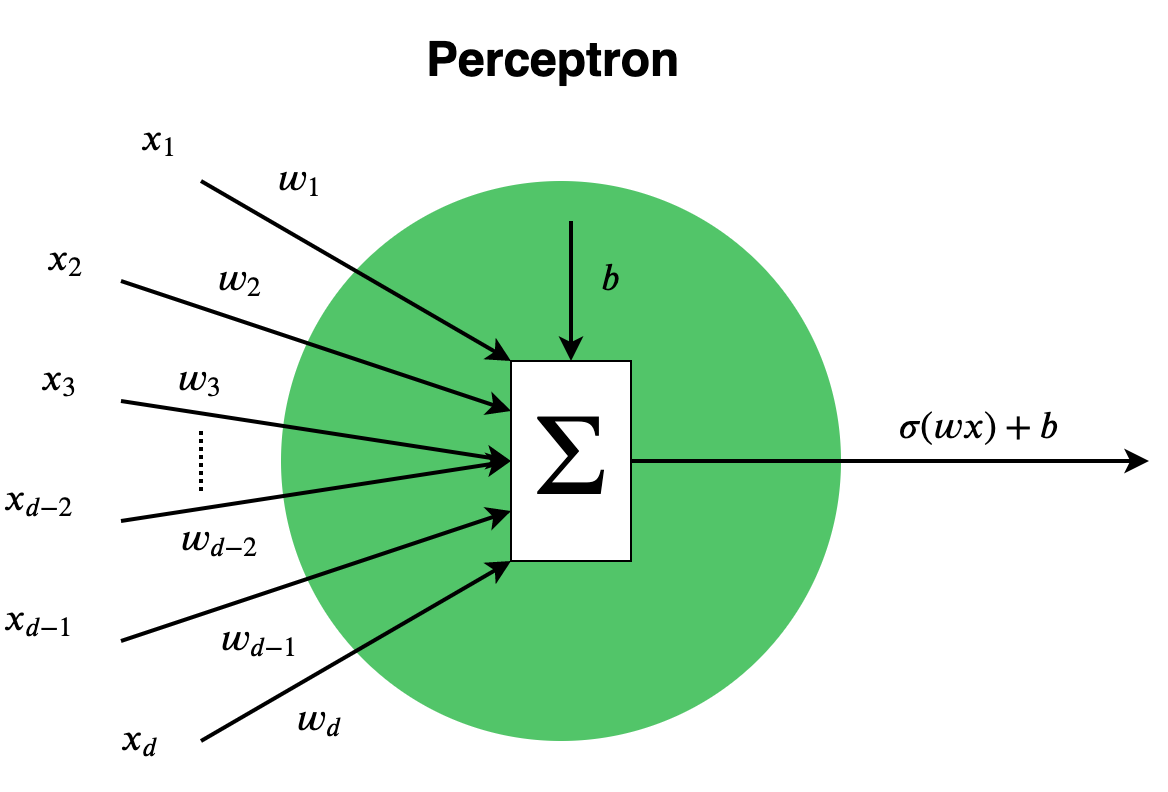
\includegraphics[width=0.8\textwidth]{img/general/perceptron.png}
	\caption{\textcolor{viridis7}{\textbf{Perceptron}} with input $x$ of dimension $d$, trainable weights $w$ and the bias $b$. The output is a linear combination of the weights and the input plus the bias. Commonly, an activation function, here denoted by $\sigma$, is applied to the output to limit the range (usually $\sigma$ refers to the \textit{Sigmoid} activation function that squeezes the output between $-1$ and $1$).}
	\label{fig:perceptron}
\end{figure}

Usually, the input is denoted by $x$ and is a vector of size $d$. The input is then summed up by the perceptron. To enable the perceptron to learn, each input also gets attached a \textit{weight}, denoted by $w$, which is multiplied by the input before summing them up. Also, a bias $b$ is added. This enables the perceptron the learn the \textit{intercept} of a linear function.

The next step in building a neural network is to combine multiple perceptrons to a network. The resulting model is mostly either called \textit{Feed Forward Network} (FFN) or \textit{Multi-Layer Perceptron} (MLP). Figure \ref{fig:neural_network} shows a simple neural network, consisting of multiple layers with multiple perceptrons.

\begin{figure}[hbt]
	\center
	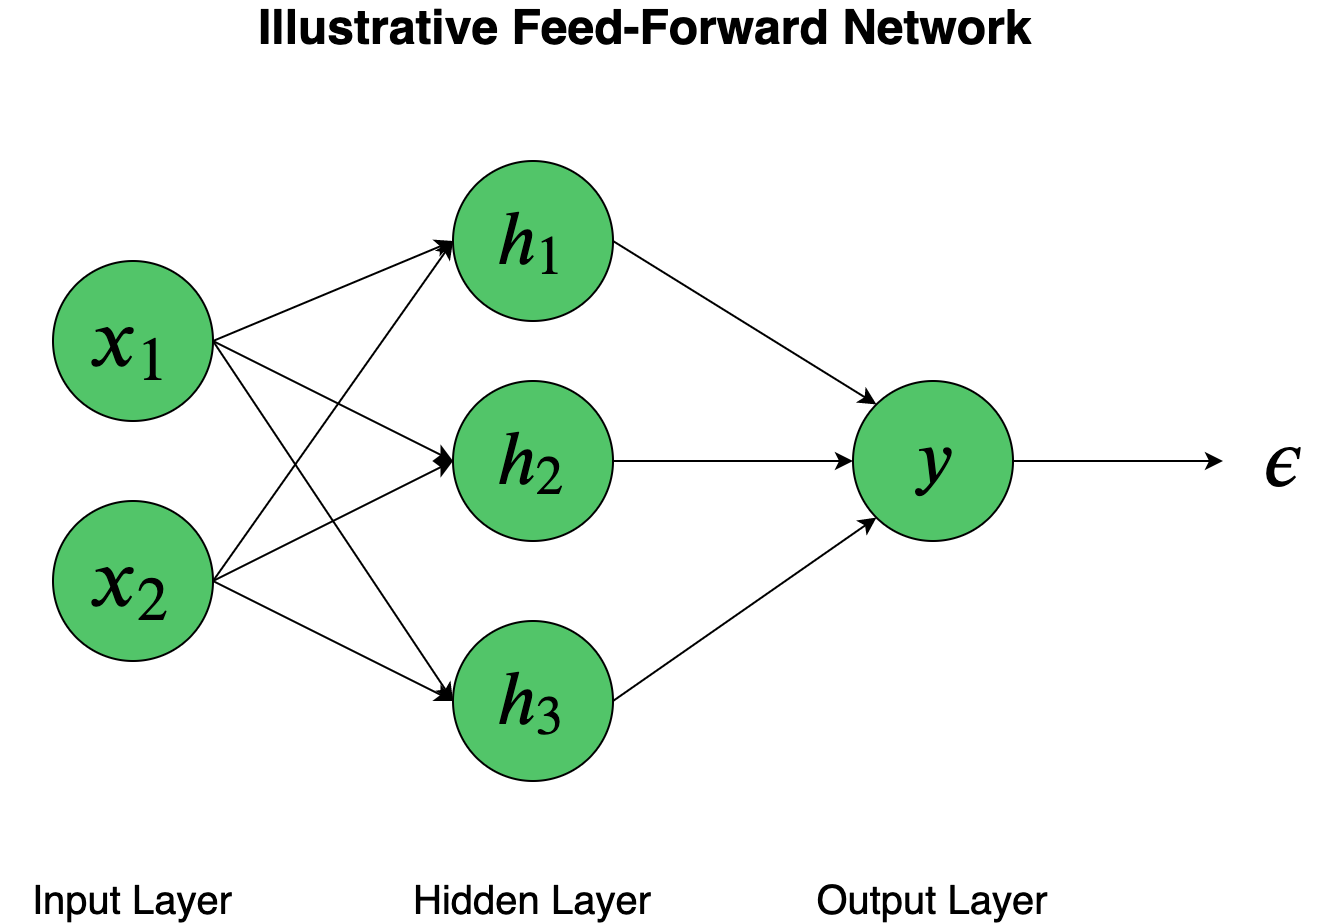
\includegraphics[width=0.9\textwidth]{img/general/neural_network.png}
	\caption{Illustrative \textcolor{viridis7}{\textbf{feed-forward neural network}}.}
	\label{fig:neural_network}
\end{figure}

The first layer is called the \textit{input} layer, the intermediate layers are called \textit{hidden} layers and the last layer is called the \textit{output} layer. The mathematical operations are conducted using a vectorised form, thus the dimensionality of $x$ is usually $n \times d$ where $n$ denotes the number of observations and $d$ the dimensionality of the input. A \textit{forward} pass then consists of calculating:

\begin{equation}
    h(x) = \sigma(x^T w_1)
\end{equation}

and

\begin{equation}
    y(h) = \sigma(h^T w_2)
\end{equation}

In these equations, $w_1$ and $w_2$ hold the weights of the layers, including the bias, making it easier using vectorised operations. $\sigma$ defines the \textit{Sigmoid} activation function which maps the output between $(-1, 1)$, see equation \ref{eq:activation_sigmoid}. Other activation functions can applied as well. The next step is to define a \textit{loss} function and then use \textit{backpropagation} the update the weights of the neural network.

The loss function defines the error of the neural network and depends heavily on the use case, for example, regression or classification. In the case of regression, the error is usually assumed to be normally distributed around the prediction $y$, therefore, the maximum likelihood estimate for the normal distribution is being optimised. This is done by maximising the \textit{mean squared error} (MSE), where $y$ denoted the true value and $\hat{y}$ the estimate of the network:

\begin{equation}
	\label{eq:mse}
    \epsilon(\hat{y}) = \frac{1}{n} \sum_{i=1}^{n} (\hat{y} - y)^2
\end{equation}

Having the loss defined, it is possible to calculate the gradient with respect to each weight and then update it accordingly. During each update, the learning rate $\alpha$ defines how much the weights are being updated. A neural network might see the training dataset multiple times during its training process. How often it sees the training dataset is referred to as \textit{iterations} or \textit{epochs}. In practice, more advanced \textit{optimisers} are used, also using \textit{momentum}. For explanatory purposes, a simple gradient update is being assumed. We are interested in the gradient of the error function with respect to each weight:

\begin{equation}
    \nabla \epsilon = \left(\frac{\delta \epsilon}{\delta w_n}, \frac{\delta \epsilon}{\delta w_{n-1}},\: ...\:, \frac{\delta \epsilon}{\delta w_1} \right)
\end{equation}

Then, to compute the gradient, the \textit{chain rule} is being applied. For $w_2$ the unfolded chain rule results in:

\begin{equation}
    \frac{\delta \epsilon}{\delta w_2} = \frac{\delta \epsilon}{\delta \hat{y}} \frac{\delta \hat{y}}{\delta h} \frac{\delta h}{\delta w_2}
\end{equation}

Finally, the respective weight is being updated according to:

\begin{equation}
    w_2^{\text{updated}} = w_2 - \alpha \odot \frac{\delta \epsilon}{\delta w_2}
\end{equation}

Here, $\odot$ defines the \textit{Hadamard product} and $\alpha$ the \textit{learning rate} which influences by how much the gradients are being updated. In practice, the gradients are calculated via numerical optimisation, thus allowing arbitrary structures of the neural network without requiring to derive an analytical solution each time the structure of the network is altered. The choice of the structure and therefore the amount of tuneable parameters heavily depends on the problem to solve. Neural networks with a lot of layers are prone to the vanishing gradient problem [\cite{pascanu2012difficulty}], which is one of the reasons that different types of neural networks are used for more complex problems. Some of them, which are used in this thesis, will be investigated in the following chapters.

\FloatBarrier
\subsection{Convolutional Neural Networks}

Convolutional Neural Networks (CNNs) are primarily used for extracting features from inputs where parts of the input are highly correlated to the parts next to it. Therefore CNNs are used, amongst others, for feature extraction in images which are then used for downstream tasks of classification or regression. Theoretically, a traditional FFN is also capable of processing images, but the amount of weights required is a magnitude higher compared to CNNs, as CNNs use the same set of weights for the whole image instead of having one weight for each pixel. Mathematically speaking, a CNN uses convolutions on a discrete input, by learning a set of weights for different filters. For the following examples, we will look at the feature extraction of a black and white image, thus a two-dimensional input.

\begin{figure}[hbt]
	\center
	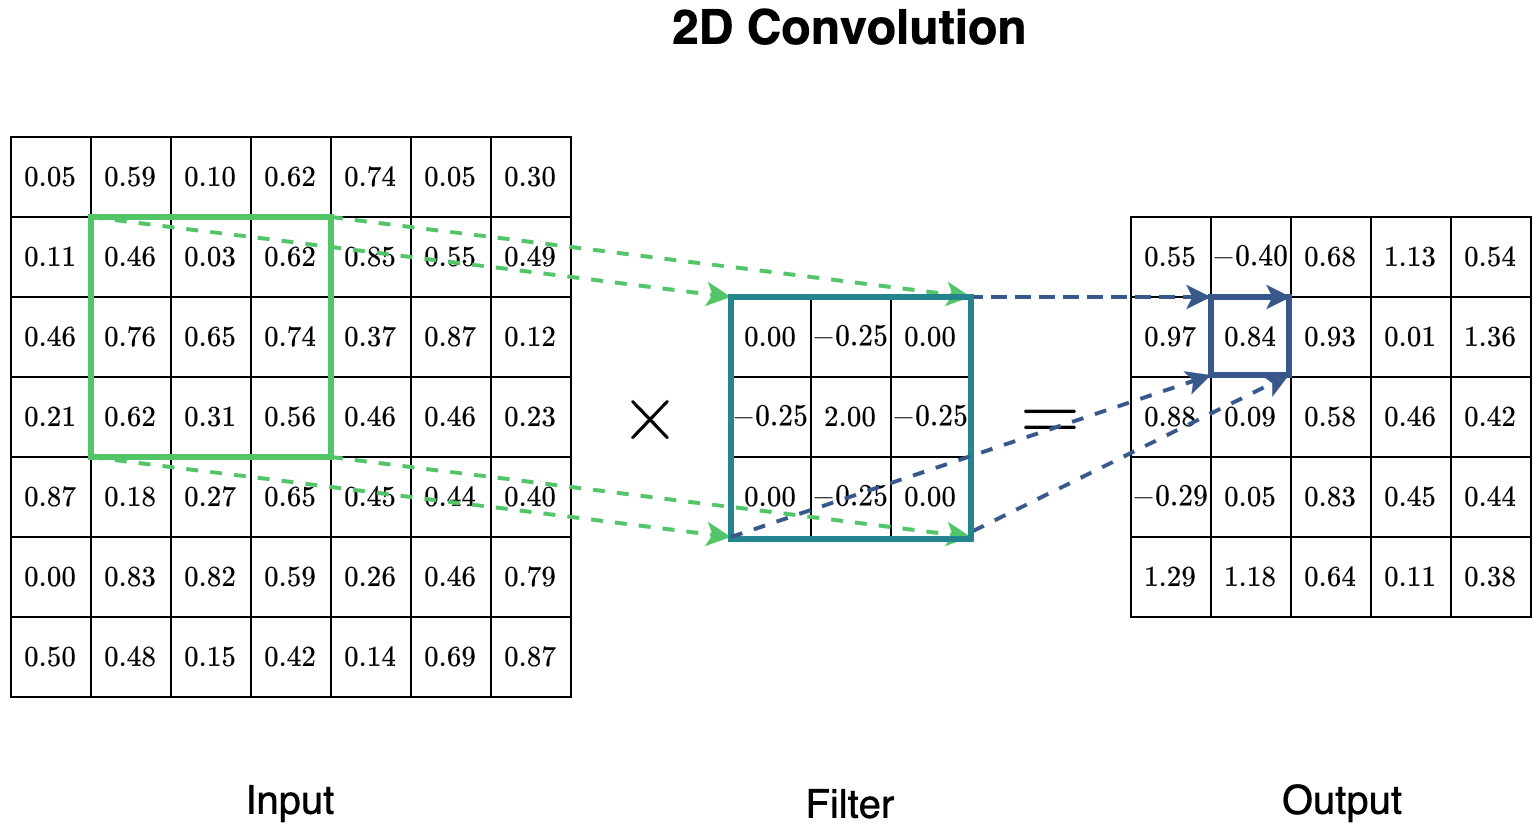
\includegraphics[width=1.0\textwidth]{img/general/convolution.png}
	\caption{2D convolution. The dot product between the \textcolor{viridis7}{\textbf{input}} and the learnable \textcolor{viridis5}{\textbf{filter}} is being calculated to produce the \textcolor{viridis2}{\textbf{output}}.}
	\label{fig:convolution}
\end{figure}

The brightness of each pixel is usually mapped to a value between $0$ and $1$ for normalisation. An example of this can be seen in figure \ref{fig:convolution}. The CNN then applies a filter to the input which can be imagined as a sliding window that is hovered over the input. During each step, the dot product between input and filter is being calculated. Note that in this case, the shapes of input and filter would be $1\times9$ and $9\times1$ respectively, thus resulting in an output value of shape $1\times1$, even if the original image is assumed to be two-dimensional. Intuitively, one could assume that the dot product between a $3\times3$ and a $3\times3$ matrix is being taken, which is not the case. Applying this filter to each sliding window of the input, the output, which is displayed on the right side, is being calculated. In this example, the filter is always moved by 1 cell, which is referred to as having a \textit{stride} of 1. To reduce the output size further, the stride could be increased. It can be noticed that the output will always be smaller than the input. To prevent this, if not desired, the input can also be \textit{padded}, usually with zeros, so that the moving window will also cover the outer regions if the stride is not a multiple of the dimensionality.

Mathematically, this operation is called a convolution and for the 2-dimensional space defined by the following equation, where $x$ is the input at location $i$ and $j$, $\mathcal{F}$ the filter values, $m$ the filter size and $s$ the stride.

\begin{equation}
	y_{ij} = \sum_{a=0}^{\lfloor m/s \rfloor} \sum_{b=0}^{\lfloor m/s \rfloor} x_{1+as, j+bs} \mathcal{F}_{a,b}
\end{equation}

In the case of a 1-dimensional convolution, as applied for time series, the formula is reduced to:

\begin{equation}
	y_{i} = \sum_{a=0}^{\lfloor m/s \rfloor} x_{i+as} \mathcal{F}_{a}
\end{equation}

For extracting features from images, one is usually is interested in the edges of an image, thus a difference between the pixels next to each other (e.g. foreground to background, thus an \textit{edge}). Generally, only these edges are of interest. As it is also of interest to reduce the size for faster processing, a concept called \textit{pooling} is being applied in a second step. An example of \textit{maxpooling} can be seen in figure \ref{fig:maxpool}.

\begin{figure}[hbt]
	\center
	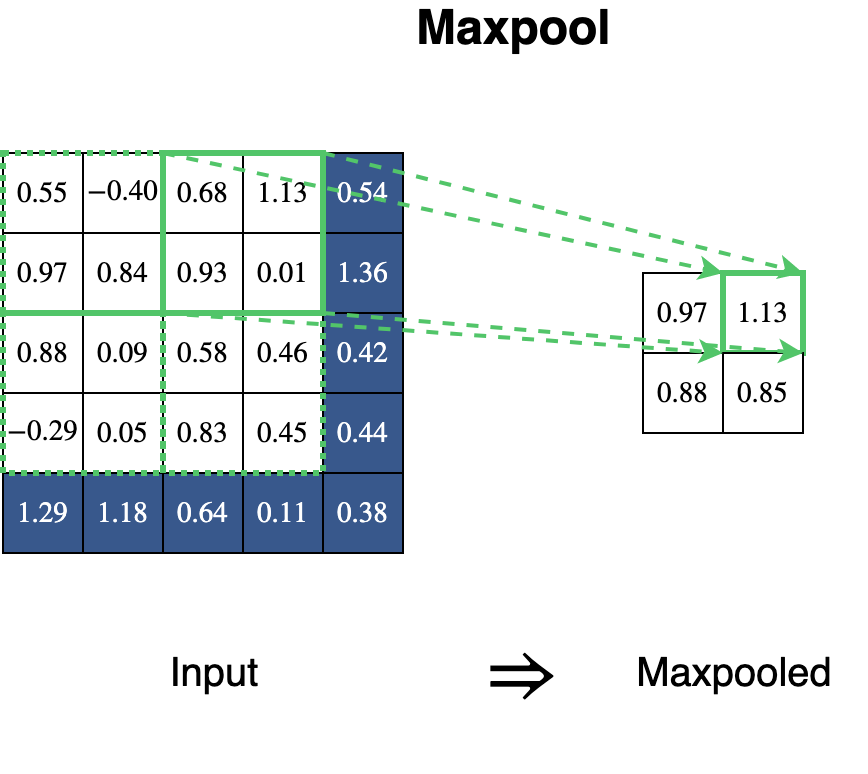
\includegraphics[width=0.65\textwidth]{img/general/maxpool.png}
	\caption{The \textcolor{viridis7}{\textbf{input}} is being maxpooled by a window of $2\times2$, thus taking the maximum of each $2\times2$ window and constructing a new tensor. The \textcolor{viridis2}{\textbf{edge cases}} are either ignored or padded with zeros, so that the \textit{max} of a windows can still be taken.}
	\label{fig:maxpool}
\end{figure}

Pooling can also be thought of as applying a sliding window with a mathematical operation applied to each window, \textit{max} in this case. During pooling, there is usually no overlap between the selected regions of the slide, indicated by the dashed line. Mostly, the edge cases are ignored, but if desired, a padding can be applied as well. Both, the pooling and the filter size, are arbitrary and thus a hyperparameter of the network. One filter applies to the whole input, so for example in this case in figure \ref{fig:convolution}, only 9 weights must be trained compared to a traditional FFN, which would have 49 trainable weights. For large images or inputs, this is a huge advantage.

The filter shown in figure \ref{fig:convolution} is a high pass filter. CNNs would be quite limited if they could only learn one filter, which would mean that they could only focus on one property of the input. For example, a filter that detects \textit{edges} where the colours shifts from black to white. Therefore, in each layer, multiple independent filter are applied and trained. For images, the first layer usually has 3 filters, one for each colour channel. To construct a whole CNN, filtering and pooling are concatenated multiple times, eventually providing features which embed information about more complex structures. These can then be used by a simpler model, for example, an FNN, for the downstream task of image classification or regression.

\subsection{Temporal Convolutional Neural Networks}

There exists no clear definition of what a Temporal Convolutional Neural Network (TCNN) exactly is. It can either be applied to multivariate time series forecasting [\cite{Wan_2019}] or classification of satellite images [\cite{pelletier2018temporal}]. In the context of this thesis, the focus will lie mainly on two modifications compared to traditional CNNs. Firstly, for classification, the cross-entropy loss function is usually used, as it produces a distribution of classes that adds up to one. The cross-entropy loss is defined as\footnote{Based on \texttt{https://pytorch.org/docs/stable/nn.html?highlight=crossentropyloss\#torch.nn.CrossEntropyLoss}}:

\begin{equation}
	\label{eq:cross_entropy}
    \text{loss}(x, \text{class}) = - \log{} \Bigg( \frac{\exp{x[\text{class}]}}{\exp{\sum_i x[i]}} \Bigg)
\end{equation}

$x[i]$ denotes the probability of the output of the model to belong to class $i$. Cross-entropy loss can also be defined in a way that it embeds weights for each class label. In this case, the loss is given by:

\begin{equation}
	\label{eq:cross_entropy_weighted}
    \text{loss}(x, \text{class}) = \text{weight}[\text{class}] \Bigg( -x[\text{class}] + \log{\bigg(  \sum_i \exp{x[i]} \bigg)} \Bigg)
\end{equation}

However, a presumed problem using cross-entropy loss is that it does not assume an order of classes. In our case of age prediction, this means that some information might be lost, as a miss-classification, which lies closer to the real age label, should be penalised less compared to one that is farther away. To take the order into account, the MSE loss, defined in equation \ref{eq:mse}, is being taken. This changes the model to a regressor. Mapping the regression output back to a class label is quite simple. For example, if the regression outputs the value $37.56$, this output would map to the class label of individuals between 30-40.

The second difference is, that compared to taking maxpooling layers, which have been described earlier, \textit{average pooling} layers are used. Contrary to detecting edges in images, time series analysis is not so much interested in the detection of edges but rather general information embedded in the time signals. Therefore, it is assumed that average pooling layers work better compared to maxpooling layers. [\cite{tcnn}, p.4] also chose to use average pooling as it seemed to work best for their set of problems. One can not say that average pooling works better than maxpooling in general for time series classification, but there is also no indication that it works worse, hence the TCNN used in this thesis is implemented using average pooling.

\subsection{Long Short-Term Memory}

Traditional Recurrent Neural Networks (RNNs) were built to handle sequences of data, where a datapoint $x_i$ is dependent on the previous data point $x_{i-1}$, thus not only on the current input of the sequence. The problem with this traditional approach is that calculating the gradients is prone to the \textit{vanishing gradient problem} [\cite{pascanu2012difficulty}]. The problem is two-folded: Firstly, the values of the gradients usually become smaller the deeper the network is, thus layers that are close to the output learn faster compared to layers closer to the input. This could be circumvented by longer training times, but raises issues with overfitting. Secondly, if the gradients become too small, it becomes computationally infeasible to represent these values in memory, as even double-precision floating-point numbers reach their limit quickly given long sequences. RNNs are specifically prone to longer input sequences.

\begin{figure}[hbt]
	\center
	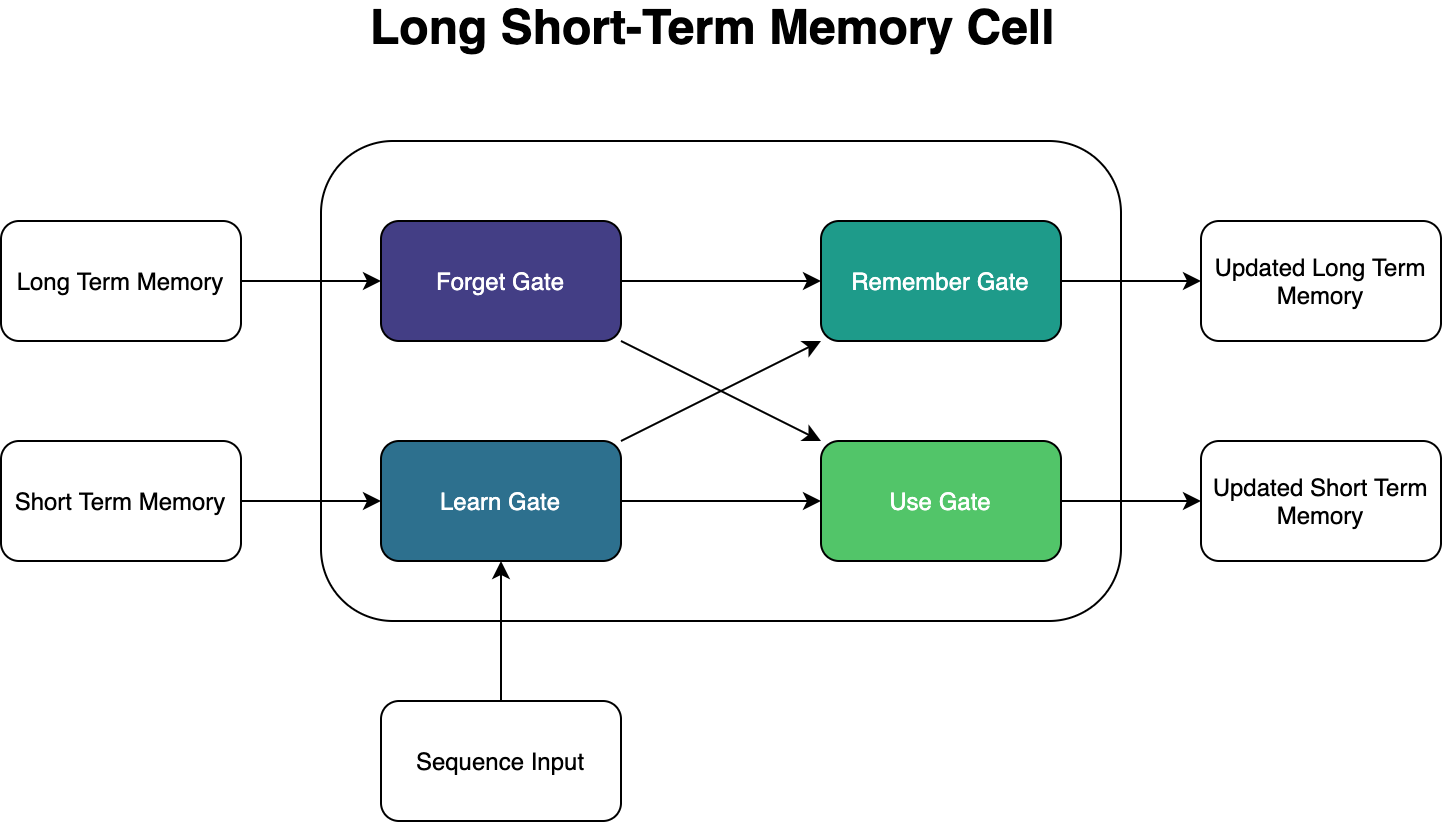
\includegraphics[width=1.0\textwidth]{img/general/LSTM.png}
	\caption{An LSTM consists of four gates. The \textcolor{viridis1}{\textbf{forget gate}} takes the previous long-term memory and decides which information to discard. The \textcolor{viridis3}{\textbf{learn gate}} looks at the previous short term memory and the input of the current sequence and decides which information is forwarded. The \textcolor{viridis5}{\textbf{remember gate}} is responsible for updating the long-term memory based on the information given from the two previous gates. The \textcolor{viridis7}{\textbf{use gate}} also looks at the output of the two previous cells, but focuses on updating the short term memory, thus the information which is used at the current point in time.} 
	\label{fig:lstm}
\end{figure}

[\cite{10.1162/neco.1997.9.8.1735}] proposed an architecture for an RNN which handles long sequences way better compared to their original counterparts. They proposed the so-called Long Short-Term Memory (LSTM) as it is particularly capable of handling long sequences. An LSTM consists of cells which have different functionalities for deciding which information to keep and which to discard. Figure \ref{fig:lstm} shows the high-level layout of such a cell. In each time step, thus for each element of the input sequence, the LSTM cell processes the new element in accordance to its internal state. This internal state consists of the Long-Term Memory (LTM) and the Short Term Memory (STM). Given the new element of the sequence, these internal status are updated in each step. The required calculations are carried out by four gates. The \textit{forget gate} looks at the LTM and decides which information is being forgotten and thereby which information is preserved for further processing. Similarly, the \textit{learn gate} looks at the STM, also often called \textit{hidden state}, as well as the current element of the sequence and decides which information is relevant for further processing. In a next step, the \textit{remember gate} sees both outputs of the previous gates and is responsible for saving long-term information in the LTM, which is updated accordingly. The \textit{use gate} filters the information which is important for usage at the given time step and saves that information in the STM.

\begin{figure}[hbt]
	\center
	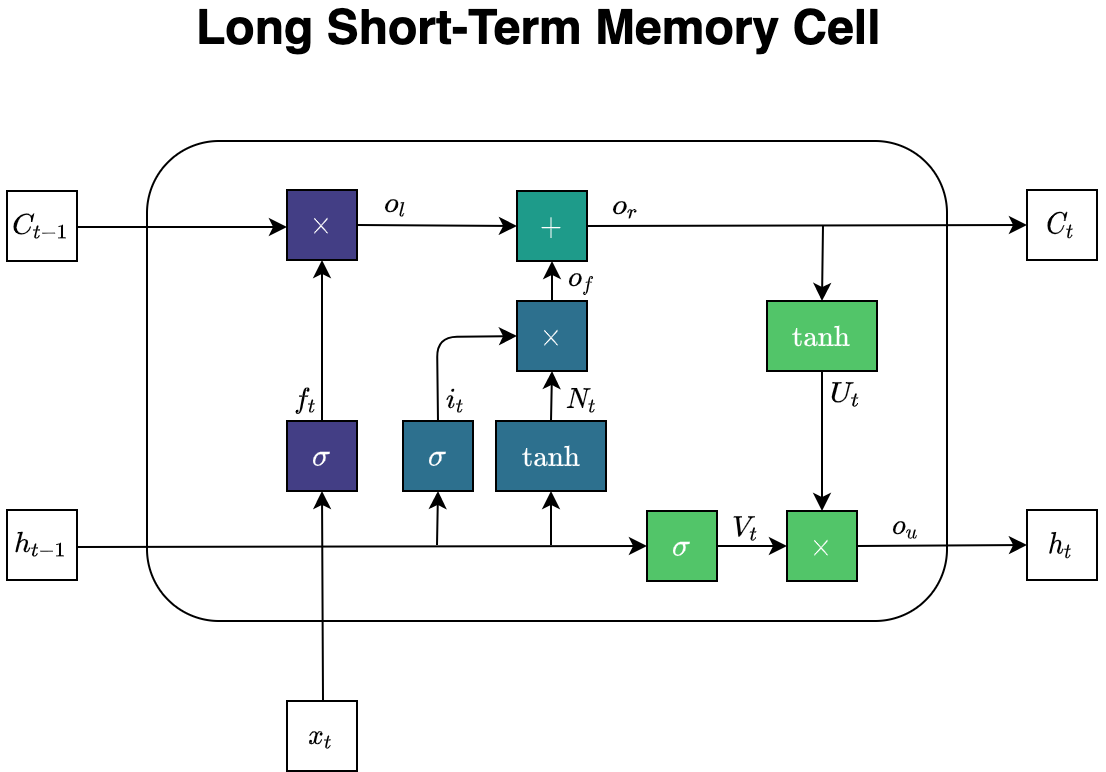
\includegraphics[width=0.8\textwidth]{img/general/LSTM-detailed.png}
	\caption{The four gates are coloured in the same way as in figure \ref{fig:lstm}. The figure shows the mathematical operations applied to the inputs of the cell. The \textcolor{viridis1}{\textbf{forget gate}} calculates the dot product between the LTM and the concatenation of the hidden state (STM) and the input $x_t$. The \textcolor{viridis3}{\textbf{learn gate}} concatenates the short term memory $h_{t-1}$ with the current input $x_t$ as well and then calculates a state and a \textit{forget factor}, which are then combined by multiplication. The \textcolor{viridis5}{\textbf{remember gate}} simply concatenates the output of the \textcolor{viridis1}{\textbf{forget gate}} and the \textcolor{viridis3}{\textbf{learn gate}}. The \textcolor{viridis7}{\textbf{use gate}} takes the output of the \textcolor{viridis5}{\textbf{remember gate}} and calculates the product between with the concatenation of the STM $h_1$ and the current sequence input $x_t$. Every step is explained in more mathematical detail in the surrounding text.}
	\label{fig:lstm-detailed}
\end{figure}

Given this high-level picture of an LSTM, the next step is to mathematically describe the calculations which are carried out by the LSTM. Figure \ref{fig:lstm-detailed} shows a more detailed version of an LSTM cell, where each gate coloured according to figure \ref{fig:lstm}. The previous LTM is denoted by $C_{t-1}$ and the previous STM, or hidden state, is denoted by $h_{t-1}$, the updated states $C_t$ and $h_t$ respectively. The current element at time step $t$ is denoted by $x_t$. Inside of the cell, mainly four calculations are conducted: Firstly, normalising the input by using an activation function which is either the \textit{Sigmoid} ($\sigma$) or \textit{tanh} ($\text{tanh}$) activation function; see equation \ref{eq:activation_sigmoid} and \ref{eq:activation_tanh}. Secondly, the dot product between two tensors ($\times$). Thirdly, the concatenation of two vectors which is denoted by two merging arrows (an intersection) in the figure and by $\langle \rangle$ in the formulas. Fourthly, the sum of two vectors ($+$). Having all variables and operations defined, we take a look at the different gates and how they work in detail.

\begin{equation}
\label{eq:activation_sigmoid}
	\sigma(x) = \frac{1}{1 + \exp(-x)} = \frac{\exp(x)}{\exp(x) + 1}
\end{equation}

\begin{equation}
\label{eq:activation_tanh}
	\text{tanh}(x) = \frac{2}{1 + \exp(-2x)} -1
\end{equation}

\paragraph*{\textcolor{viridis3}{\textbf{Learn Gate}}}
First, the current element $x_t$ is being taken and concatenated with the current STM $h_{t-1}$. Then, the dot product between this resulting vector and the weights $W_n$ of the learn gate is being calculated, before the tanh activation function is being applied. Let $N_t$ denote this intermediate result. Furthermore, the \textit{ignore factor} $i_t$ is being calculated by applying the Sigmoid activation function to the dot product between additional weights $W_i$ and the same concatenation of $x_t$ and $h_{t-1}$ as before. The output of the learn gate is then defined as the dot product $N_t i_t$.

\begin{equation}
	N_t = \text{tanh}(W_n \langle h_{t-1}, x_t\rangle)
\end{equation}

\begin{equation}
	i_t = \sigma(W_i \langle h_{t-1}, x_t\rangle)
\end{equation}

\begin{equation}
	\text{o}_{l} = N_t i_t
\end{equation}

\paragraph*{\textcolor{viridis1}{\textbf{Forget Gate}}}
Similarly to the learn gate, the dot product between a set of weights $W_f$ and the concatenation of $x_t$ and $h_{t-1}$ is passed to the Sigmoid activation function. Let this value, also called \textit{forget factor}, be denoted by $f_t$. The output of the forget gate is then defined by the dot product between $f_t$ and the LTM $C_{t-1}$.

\begin{equation}
	f_t = \sigma(W_f \langle h_{t-1}, x_t\rangle)
\end{equation}

\begin{equation}
	\text{o}_{f} = C_{t-1} f_t
\end{equation}

\paragraph*{\textcolor{viridis5}{\textbf{Remember Gate}}}
Simply, the output of the learn gate $o_l$ is summed with the output of the dot product of the LTM $C_{t-1}$ and the forget factor $f_t$ of the forget gate.

\begin{equation}
	o_r = o_l + o_f
\end{equation}

\paragraph*{\textcolor{viridis7}{\textbf{Use Gate}}}
The tanh activation function of the dot product between a set of weights $W_u$ and the output of the forget gate $o_r$ is being calculated. Let this value be denoted by $U_t$. Additionally, the value $V_t$ is being calculated by taking the Sigmoid activation of the dot product between a set of weights $W_v$ and the concatenation of $h_{t_1}$ and $x_t$ again. Followingly, the output is defined as the product of $U_t$ and $V_t$.

\begin{equation}
	U_t = \text{tanh}(W_u o_r)
\end{equation}

\begin{equation}
	V_t = \sigma(W_v \langle h_{t-1},x_t\rangle)
\end{equation}

\begin{equation}
	o_u = U_t V_t
\end{equation}

Inferring from the descriptions of the gates and figure \ref{fig:lstm-detailed}, the new LTM $C_t$ is defined by $o_r$ and the new STM, or hidden state, $h_t$ is defined by $o_u$. The whole LSTM cell then behaves like a traditional RNN, where each element of the sequence is being processed and the different states are updated accordingly. Figure \ref{fig:lstm-sequence} shows three cells of the unfolded sequence.

\begin{figure}[hbt]
    \makebox[\linewidth][c]{
	\centering
	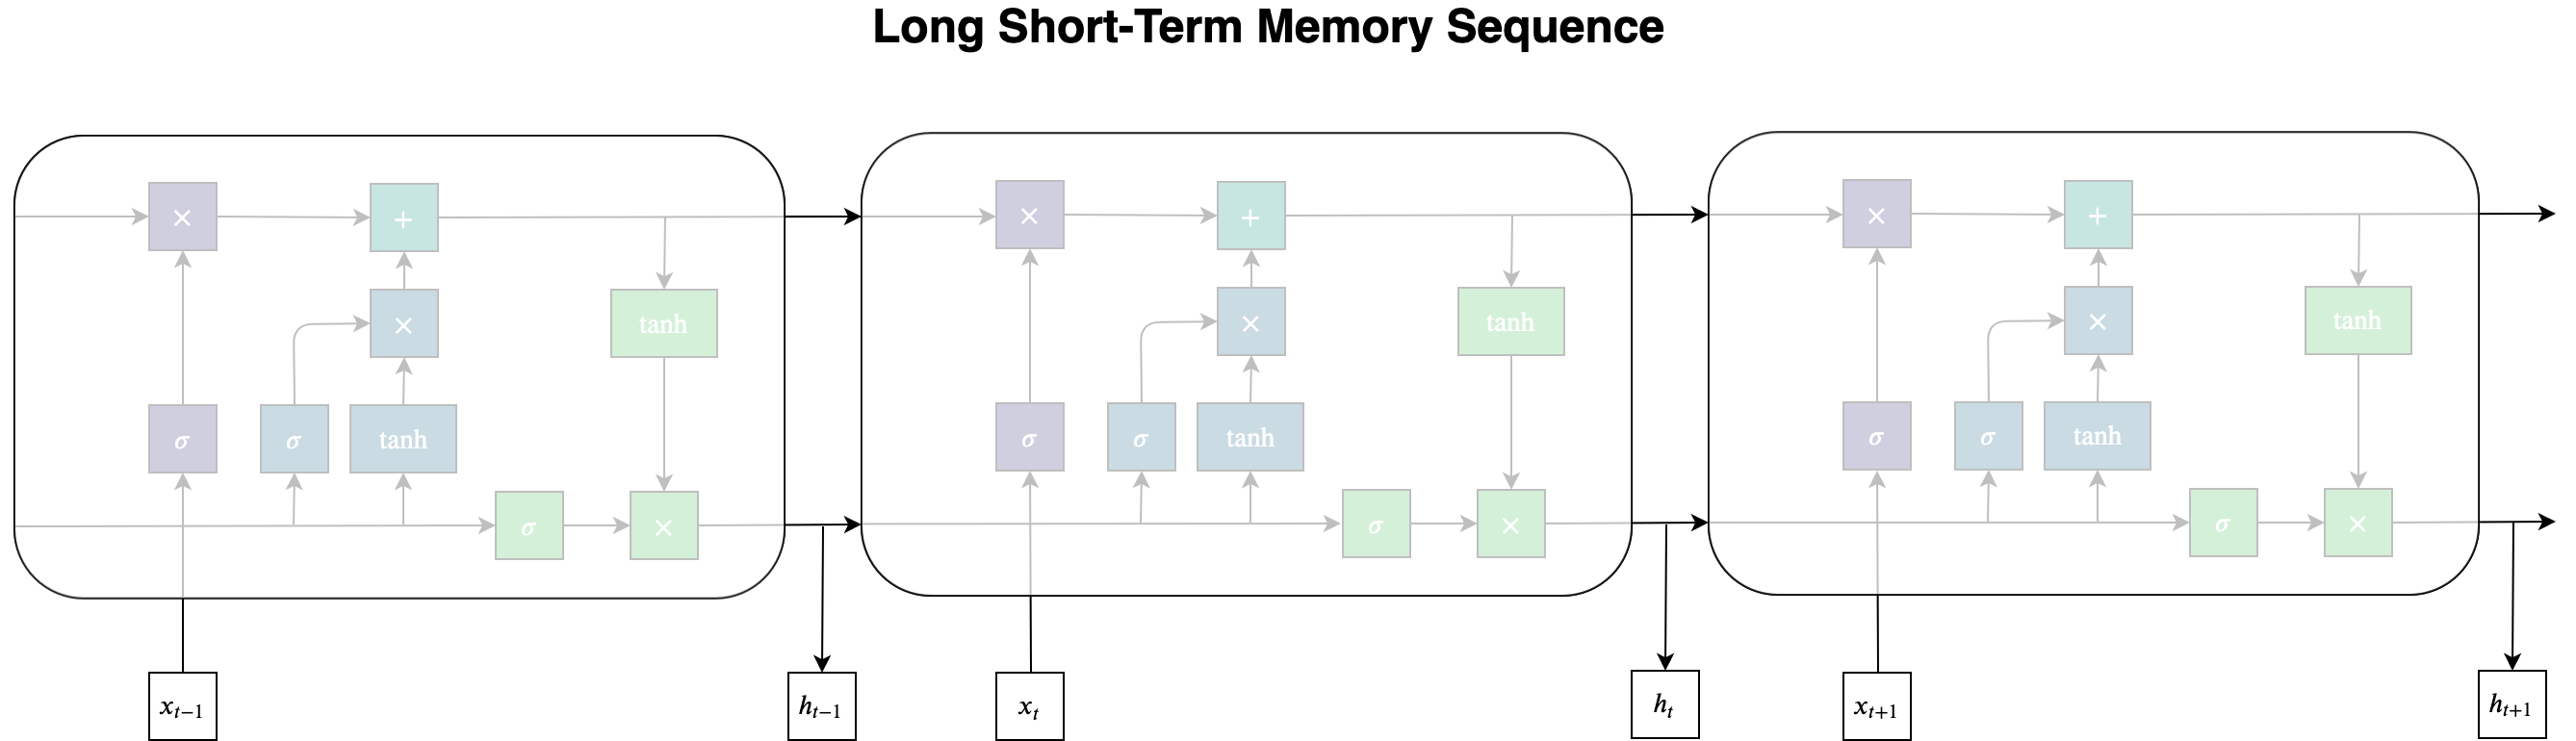
\includegraphics[width=1.2\textwidth]{img/general/LSTM-sequence.png}
	}
	\caption{Multiple LSTM cells unfolded resemble a sequence, where each state is passed on to the next cell. This continues until the whole input sequence $x_t$ is processed. This is related to the function of a classical RNN, but LSTMs do not suffer that much from vanishing or exploding gradient and are thus better in learning long-term dependencies in the input sequence.}
	\label{fig:lstm-sequence}
\end{figure}

Apart from the fact that it is easier for an LSTM to store long-term dependencies, the training history of an LSTM is not completely dependent on each previous operation. It only depends on the previous states, thus completely decoupling the calculations of the gradients for each input from its history. Therefore, LSTMs are less prone to the vanishing gradient problem. In practice, the gradients are automatically calculated. PyTorch\footnote{https://pytorch.org/} does this by applying \textit{reverse mode automatic differentiation} [\cite{paszke2019pytorch}].

\FloatBarrier
\subsection{Linear Spline Interpolation}

Missing data can be handled in multiple ways. A simplistic approach is the usage of spline interpolation. Splines define a piecewise polynomial function between two points of a series, also called nodes. Hence, missing data points can be calculated using the interpolated polynomial function. The most elementary polynomial function is of first order, thus only forcing the function values of adjacent nodes to be equal. Inferentially, defining a linear function. A second-order polynomial also defines the first derivative of the nodes to be equal and is hence called quadratic interpolation. Concludingly, speaking of a cubic interpolation, the second derivate has to be equal as well. The same applies for higher polynomials for interpolation.

As the computational costs of computing splines is quite high, this thesis will only focus on linear spline interpolation. Higher orders have been tested as well but take too much time, especially considering that the interpolation is still way too simple to account for the patterns in the time series. Figure \ref{fig:slice_raw_data} shows a slice of a time series which will also be used in further chapters as an example for data interpolation and simulation.

\begin{figure}[hbt]
	\center
	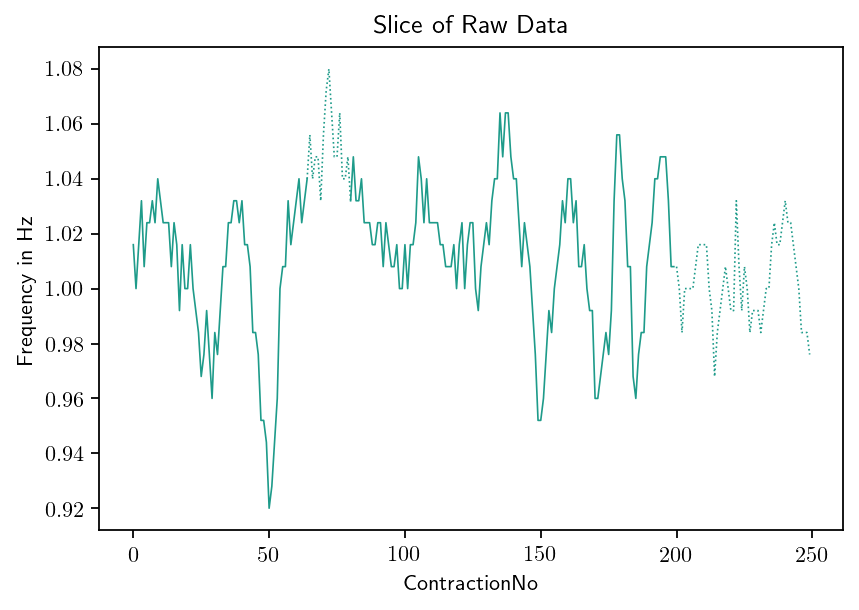
\includegraphics[width=1.0\textwidth]{img/general/slice_raw_data.png}
	\caption{Example \textcolor{viridis5}{\textbf{slice of the data}}. Dotted lines are missing or padded data points.}
	\label{fig:slice_raw_data}
\end{figure}

Let $x_i$ denote the \textit{it}h data point in the given series. Then, a linear spline between $x_i$ and $x_{i+1}$ is defined by\footnote{\textbf{Source:} \url{https://www.math.uh.edu/\~jingqiu/math4364/spline.pdf}}:

\begin{equation}
	s(x) = f(x_i) \frac{x - x_{i+1}}{x_i - x_{i+1}} + f(x_{i+1}) \frac{x - x_i}{x_{i+1} - x_i}
\end{equation}

Given $s(x)$, the domain between $x_i$ and $x_{i+1}$ can be evaluated at any point. Figure \ref{fig:slice_raw_data_linear_spline_interpolation.png} shows the linear spline interpolation applied to the exemplary slice. It can be seen that the fit is not very good, but enables us to pass the data to models for inference. It can also be seen, that for missing data at the end of a series, the last value is just being repeated as the right-hand values are missing due to padding. This arises from the fact that, for enabling batch processing, all input vectors must have the same length.

\begin{figure}[hbt]
	\center
	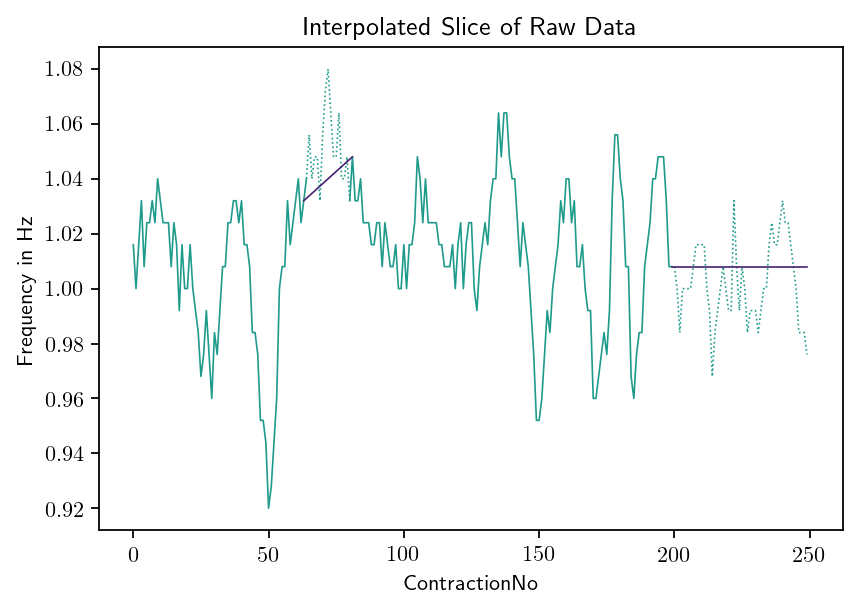
\includegraphics[width=1.0\textwidth]{img/general/slice_raw_data_linear_spline_interpolation.png}
	\caption{Example \textcolor{viridis5}{\textbf{slice of the data}} used for \textcolor{viridis0}{\textbf{linear interpolation}} and fitting a $\mathcal{GP}$. Dotted lines are missing data points not seen during interpolation or fitting of the $\mathcal{GP}$.}
	\label{fig:slice_raw_data_linear_spline_interpolation.png}
\end{figure}

\FloatBarrier
\subsection{Gaussian Processes}

Gaussian Processes ($\mathcal{GP}$s) are fully defined by a multivariate Normal distribution over a continuous input space, which is primarily defined by a finite number of observations [\cite{10.5555/1162254}, p. 13]. A $\mathcal{GP}$ can be evaluated at any set of index points, providing a comfortable way of evaluating points which were originally not present in the observations. Also, as the GP itself is a distribution, it can be used to obtain multiple samples from the fitted process. Therefore, $\mathcal{GP}$s can be used for tackling the following three challenges concerning RR intervals.

Firstly, recordings may have missing data points and while using polynomial functions helps to mitigate some of the arising issues, this approach fails to capture the underlying nature of the process. For example, using splines, a feature defined by the mean of the time series, will most likely be not that much affected whereas features that utilise the frequency domain are more prone to simple interpolation techniques. Secondly, deep learning models benefit strongly from the availability of a lot of training data. Having a defined distribution at hand, samples can be easily taken to artificially create more training data. The sampled data might be highly correlated, but still adds more variability compared to only using the original data while also accounting for the uncertainty and thereof the variability of the data. Another effect of this is, that less epochs are required for training the model which might lead to less overfit. CNNs for image classification work in a similar way by cropping and rotating the input images to enable the model to generalise better. Thirdly, to achieve a high throughput during the training of deep learning models, a fixed input shape is highly beneficial. Depending on the definition of the model, this is indispensable. While even perfectly recorded data has the issue, that due to the nature of a different pace of heart contractions, the recorded samples vary in length. Samples taken from a $\mathcal{GP}$ can be forced to always have the same length. For mitigating this third challenge, other approaches might be considered as well, but as $\mathcal{GP}$s incorporate the handling fo all three issues, they will be favoured and further investigated.

As a $\mathcal{GP}$ is a multivariate Normal distribution, it is fully defined by its mean $\mu_D$ and a covariance matrix $\Sigma_D$, where $D$ defines the amount of observations and thus the discrete dimensionality. Let the set of observations be denoted by $\chi$ and let the corresponding $y = f(\chi)$ be assumed to be known for all observations. Then, the mapping function can be written as:

\begin{equation}
\label{eq:gp_basic}
    f(x) \sim \mathcal{GP}(\mu_D, \Sigma_D)
\end{equation}

As $\mu_D$ is not compelled to be a constant value, it can be defined by a function itself, only depending on $x$. $x$ is used instead of $\chi$ to underline that this function can be evaluated for any input at any time. In practice, $x$ will be replaced by the predictive index points. We will let $\mu_D$ be defined by the following mean function:

\begin{equation}
\label{eq:gp_mean}
    \mu_D = m(x)
\end{equation}

For constructing the covariance function, the \textit{Kernel Trick} [\cite{10.5555/3008751.3008793}] is exploited to calculate the dot product in higher-dimensional space. Therefore, the covariance matrix $\Sigma_D$ is defined by a \textit{kernel function} which defines the similarity between different points in the input space. The sum or product of two kernels is still a kernel [\cite{shawe-taylor_cristianini_2004}, Proposition 3.22 (Closure Properties)]. This property can be used to combine different kernels to describe the given observations accurately and hence capturing the underlying natural process. Concludingly, the covariance matrix is given by the \textit{gram matrix}, which defines the distances, based on the given kernel function, between all combinations of observations. This matrix will be further referred to as the \textit{kernel matrix} which must be symmetric and positive-definite [\cite{10.5555/1162254}, ch. 4]. The covariance matrix is defined by the following equation:

\begin{equation}
\label{eq:gp_variance}
    \Sigma_D = k(\chi, \chi)
\end{equation}

Using definitions \ref{eq:gp_mean} and \ref{eq:gp_variance}, we can refine \ref{eq:gp_basic} to:

\begin{equation}
    f(\chi) \sim \mathcal{GP}\big(m(x), k(\chi, \chi)\big)
\end{equation}

The whole statistical model is then defined by the following equation, where $y$ denotes the output of the model:

\begin{equation}
    y = \mathcal{N}\big(f(\chi), \sigma_{\text{noise}}\big)
\end{equation}

where the observations are assumed to be normally distributed around the mapping function (defined by the $\mathcal{GP}$) and $\sigma$ defines the noise of the observations. 

By this definition, we acquired the desired distributions over functions which can be evaluated at any predictive point. Let $\chi^\ast$ denote this set of predictive points and let us refer to the evaluation of these points as \textit{regression} or \textit{prediction}. Let $k(...)$ denote the kernel function for obtaining the covariance matrix. To actually compute the predictions, first, the prior joint distribution between the observations $f(\chi)$ and $f(\chi^\ast)$ must be defined [\cite{10.5555/1162254}, eq. 2.21]:

\begin{equation}
    \begin{bmatrix}
    y \\
    f(\chi^\ast)
    \end{bmatrix}
    \sim
    \mathcal{N} \Bigg(m(x),
        \begin{bmatrix}
        k(\chi, \chi) + \sigma_{\text{noise}}^2I & k(\chi, \chi^\ast) \\
        k(\chi^\ast, \chi) & k(\chi^\ast, \chi^\ast)
        \end{bmatrix}
    \Bigg)
\end{equation}

Note that $y = f(\chi)$ as the noise of the observations is already included in the
covariance matrix. Then, we condition on the observations [\cite{10.5555/1162254}, eq. 2.22, 2.23, 2.24] to obtain the predictive distribution:

\begin{equation}
\label{eq:gp_fitted}
\begin{split}
     f(\chi^\ast) | \chi^\ast, \chi, f(x) \sim \mathcal{N} \big(
    \bar{\chi_\ast}, \text{cov}(\chi_\ast)
    \big)
\end{split}
\end{equation}

\begin{equation}
    \label{eq:gp_fitted_mean}
    \bar{f_\ast} = k(\chi^\ast, \chi) \big(k(\chi, \chi) + \sigma_{\text{noise}}^2I\big)^{-1}y
\end{equation}

\begin{equation}
    \label{eq:gp_fitted_covariance}
    \text{cov}(f_\ast) = k(\chi^\ast, \chi^\ast) - k(\chi^\ast, \chi) \big( k(\chi, \chi) + \sigma_{\text{noise}}^2I \big)^{-1} k(\chi, \chi^\ast)
\end{equation}

Note that this predictive distribution assumes a zero mean, thus $m(x)$ must be subtracted first before applying the formula. Having the predictive distribution defined, the process of regression is straight forward\footnote{Either implementing algorithm 2.1 from \cite{10.5555/1162254} or using a library.}. The last step is to select an appropriate kernel function. Chapter \ref{lab:kernels_and_hyperparameters} will explain in detail which kernel functions are used for the given specific problem set in this thesis.

For now, the focus will lie on the parameters that define the kernel functions, as most, if not all, kernel functions have parameters which can be tuned with respect to the given set of observations. We will generally refer to these flexible parameters as \textit{kernel hyperparameters} and denote them by $\theta$, thus $\theta$ is a set of hyperparameters. The aim is to select the hyperparameters that most accurately describe the underlying process, in our case the RR intervals. When choosing an optimisation strategy for selecting appropriate hyperparameters, computational constraints must be taken into account. The approaches can be split into two categories: A traditional approach of finding point estimates ($\hat{\theta}$) for the hyperparameters and a Bayesian approach of defining a prior on each hyperparameter and then updating our beliefs according to the given observations. When optimising traditionally, a maximum likelihood point estimate for the marginal log-likelihood function is the object of interest. The marginal log-likelihood will be introduced shortly. One way is to conduct \textit{grid search}, where the marginal log-likelihood of different combinations of hyperparameters is evaluated and the most likely set of parameters is being chosen. The drawback is that the search space might be tremendously large, yielding in very long run times. When limiting the search space, appropriate point estimates might not be found. To circumvent this issue, \textit{gradient descent} [\cite{gradientdescent}] will be considered for retrieving point estimates for the set of hyperparameters. The Bayesian approach marginalises the hyperparameters, thus integrating out the parameters, to obtain a \textit{posterior predictive distribution}, which can then be used to sample from. The benefit of the Bayesian approach is that the uncertainty will be taken into account. The following two sub-chapters will formalise and investigate both approaches.

\subsubsection{Kernel Hyperparameters: Point Estimate Retrieval by Gradient Descent} \hfill

The aim is to maximise the marginal log-likelihood of the $\mathcal{GP}$ with the set of hyperparameters $\theta$. $K_\theta$ denotes the covariance matrix and $\theta$ is used as an index to emphasise its dependence on the kernel parameters. The log marginal likelihood is given by [\cite{10.5555/1162254}, eq. 2.30], which is extended by the dependency on $\theta$.

\begin{equation}
\label{eq:gp_log_marginal_likelihood}
    \mathcal{L}(y | \chi, \theta) = - \frac{1}{2}y^T \big(K_\theta + \sigma_{\text{noise}}^2I\big)^{-1}y - \frac{1}{2} \log{|K_\theta + \sigma_{\text{noise}}^2I|} - \frac{n}{2} \log{2\pi}
\end{equation}

For optimisation, it is sufficient to optimise the proportion:

\begin{equation}
\label{eq:gp_neg_log_lik}
    \mathcal{L}(y | \chi, \theta) \propto - \frac{1}{2}y^T \big(K_\theta + \sigma_{\text{noise}}^2I\big)^{-1}y - \frac{1}{2} \log{|K_\theta + \sigma_{\text{noise}}^2I|} = \mathcal{L}_{prop}(y | X, \theta)
\end{equation}

For applying gradient descent, we are interested in the gradient of the negative proportional marginal log-likelihood. Let $\Theta$ denote the amount of optimisable parameters:

\begin{equation}
    \nabla \theta = - \sum_{i=1}^{\Theta} \frac{\partial \mathcal{L}_{prop}(y | \chi, \theta_i)}{\partial \theta_i} = \bigg( -\frac{\partial \mathcal{L}_{prop}(y | \chi, \theta_1)}{\partial \theta_1}, \dots, -\frac{\partial \mathcal{L}_{prop}(y | \chi, \theta_\Theta)}{\partial \theta_\Theta} \bigg)
\end{equation}

The exact form of this equation depends on the chosen kernel. In the case of a sum of kernels, the partial derivatives are quite easy to calculate, as the terms not concluding the current $\theta$ can simply be dropped. It becomes rather complex if a product of kernels is being used. In practical usage, libraries such as PyTorch, use \textit{reverse-mode automatic differentiation} [\cite{paszke2019pytorch}], as mentioned before. Therefore, the analytical solution will be omitted at this step.

\subsubsection{Kernel Hyperparameters: Posterior Predictive Distribution} \hfill

The posterior predictive distribution is given by 

\begin{equation}
    p(\Tilde{y}|y) = \int_\theta p(\Tilde{y}|\theta, y) p(\theta|y)d\theta
\end{equation}

where $\Tilde{y}$ is a future draw given the observed data. To be able to draw samples from this posterior predictive distribution, first, a posterior draw $\theta^{(1)}$ is being taken from the joint posterior distribution $p(\theta|y)$ and then a draw from the fitted $\mathcal{GP}$ (equation \ref{eq:gp_fitted}) given $\theta^{(1)}$ is taken. This process is repeated until the desired amount of samples is reached.

As it will be computationally infeasible to fit a $\mathcal{GP}$ to the complete time series, the simulation will be based on slices of the original time series and the beliefs about the parameters will be continuously being updated. This means that first of all, a $\mathcal{GP}$ is fitted to the first splice using initial priors defined for each parameter. Then, for the second slice, the priors are given according to the posterior parameter distributions of the previous slice. Eventually, the final posterior distributions will have considered all data points of the RR interval. Let's assume our observations are split into two slices $\chi_a$ and $\chi_b$. After that, the sequential update of our beliefs can be formalised as [\cite{murphy2013machine}, p. 75]:

\begin{equation}
    p(\theta|\chi_a,\chi_b) \propto p(\chi_b|\theta)p(\theta|\chi_a)
\end{equation}

This sequential update assumes exchangeability of our data [\cite{Bernardo2001TheCO}]. As we are dealing with time series data, this assumption is violated. Still, the resulting priors are assumed to be better, compared to setting them manually for each slice, as the hyperparameter space is quite high dimensional. Also, for some kernels, it is very hard to develop a good understanding of the priors, especially considering the final joint distribution and its likelihood.

\subsubsection{Confidence and Prediction Intervals}

As the error is assumed to be normally distributed, an approximation of $\sigma_{\epsilon}=1.96$ is being taken for calculating the following 95 per cent intervals. The 95 per cent confidence interval for the mean can be evaluated for each predictive point $\chi^\ast$ and is given by:

\begin{equation}
    f_\ast^{\text{upper/lower}} = m(\chi^\ast) \pm 1.96 \sqrt{\tr \text{cov}(f_\ast)}
\end{equation}

For the 95 per cent prediction interval, the noise of the observations must be considered as well:

\begin{equation}
   y_\ast^{\text{upper/lower}} = m(\chi^\ast) \pm 1.96 \sqrt{\tr \text{cov}(f_\ast) + \sigma^2_{\text{noise}}}
\end{equation}


\clearpage
\section{Methods}

This chapter describes the different methods used for obtaining the results of this thesis. That includes a thorough description of the data pipeline.

\subsection{Preprocessing}

For conducting the task of age prediction, different approaches will be taken. The aim of these different approaches is, on the one hand, to make the previous results obtained by [\cite{patternshrd}] reproducible and on the other hand, to extract features for multiple slices of the time series as this might provide more information for the feature-based models. Therefore, each model will be trained once for the \textbf{complete} RR interval and once for \textbf{constant} slices of around 5 minutes. The expectation is, that for the DeepSleep-based model, the complete time series will lead to better results whereas the feature-based models profit from a set of features for each slice and hence more information. Additionally, the models will be trained for classification, not assuming an order of the age decades, as well as for regression, where an order of the class labels is being assumed. This leaves us with the following four combinations of preprocessed data for each dataset:

\begin{itemize}
	\item complete classification
	\item constant classification
	\item complete regression
	\item constant regression
\end{itemize}

In case of constant slices, the models will, during inference, conduct one classification for each slice and perform a majority vote for the age decade label. In case of regression, the closest age decade will be assumed as the predicted class. Concluding from the limitation that the data can only be simulated for slices, the models run on the simulated data will only cover the type constant. Recall that outliers in the \textit{CAST RR Interval Sub-Study Database} dataset (the Physionet dataset) are already dealt with during the reading process of the initial data.

Both datasets are split into training, validation and testing. For the Gdańsk dataset, the splits are set to $[0.6, 0.2, 0.2]$ as the dataset is rather small, whereas the splits for the PhysioNet dataset are set to $[0.8, 0.1, 0.1]$. The seed used for the random split is $42$. The first step of data preprocessing includes linear spline interpolation, the functionality is provided by the function \texttt{interpolate()} by the \texttt{pandas} library\footnote{\texttt{https://pandas.pydata.org/pandas-docs/stable/reference/api/pandas.Series.interpolate.html}}. In the case of slicing the time series, each RR interval is split into $48$ slices for the Gdańsk dataset and into $240$ slices for the Physionet dataset, using the function \texttt{array\_split()} provided by the \texttt{numpy} library\footnote{\texttt{https://docs.scipy.org/doc/numpy/reference/generated/numpy.array\_split.html}}.

For obtaining a closely related set of $33$ features used by [\cite{patternshrd}], the library \texttt{hrvanalysis}\footnote{\texttt{https://github.com/Aura-healthcare/hrvanalysis}} is used. The features are categorised as follows:

\begin{itemize}
	\item \textbf{Time Domain Features:} Mean\_NNI, SDNN, SDSD, NN50, pNN50, NN20, pNN20, RMSSD, Median\_NN, Range\_NN, CVSD, CV\_NNI, Mean\_HR, Max\_HR, Min\_HR, STD\_HR
	\item \textbf{Geometrical Domain Features:} Triangular\_index, TINN
	\item \textbf{Frequency Domain Features:} LF, HF, VLF, LH/HF ratio, LFnu, HFnu, Total\_Power
	\item \textbf{Non-Linear Domain Features:} CSI, CVI, Modified\_CSI, SD1, SD2, SD1/SD2 ratio, SampEn
\end{itemize}

Some of the features are not independent. For further information, please refer to either the python package or the methods chapter of [\cite{patternshrd}, p. 3].

For the DeepSleep-based model, no features are necessary, but the time series must be padded for enabling batch processing. The 95th percentile of the respective lengths distributions has been chosen as a trade-off between including the greater part of the series and padded values. The percentiles have been rounded to the next value dividable by $1,000$. This results in a padding value of $27,000$ for the Gdańsk dataset and 135.000 for the Physionet dataset. In case of the type \textbf{constant}, the paddings are divided by the number of slices, thus resulting in $462$ for the Gdańsk dataset and $2,812$ for the Physionet dataset.

\subsection{DeepSleep Architecture}

\begin{figure}[hbt]
	\center
	\includegraphics[width=0.65\textwidth]{img/general/deepsleep.png}
	\caption{DeepSleep-based architecture. The first part consists of a \textcolor{viridis1}{\textbf{CNN}} with two heads. The second part consists of an \textcolor{viridis3}{\textbf{BiLSTM}} with a concurrent \textcolor{viridis5}{\textbf{FNN}}, also denoted as \textit{Sidearm}, and the \textcolor{viridis7}{\textbf{Downstream Classifier/Regressor}} producing the output.}
	\label{fig:deepsleep}
\end{figure}
	
In addition to the feature-based models, a deep learning approach will be investigated to find out, how well this self-learning approach performs. The main difference between these types of models is that deep learning can extract features on its own and is independent of manually constructed features. Usually, deep learning models are not as interpretable as feature-based models, but can perform better under some circumstances.

[\cite{deepsleep}] proposed a deep learning architecture, consisting of a CNN for feature extraction, an LSTM for long-term dependencies and a simple FFN for the downstream task of classification and regression. Their architecture is called \textit{DeepSleep} and works directly on raw single-channel EEG data. The obtained results for sleep stage detection seem to indicate that DeepSleep is suitable for long medical time series data, as they obtained significant F1 scores on two different datasets. Therefore, the proposed architecture serves as a basis where some modifications are being applied. The architecture used in this thesis can be seen in figure  \ref{fig:deepsleep}.

The first part of the model consists of a two-headed \textcolor{viridis1}{\textbf{CNN}} with different kernel sizes, where one focuses more on longer patterns whereas the other one puts more emphasis on shorter patterns. The CNN consists of three layers. Contrary to CNNs working on image data, the kernel size and amount of filters is not changed throughout the layers. After the CNN layers, the batches are normalised and average pooling is being applied to the CNN features, which has the same size as the filters. After concatenating both strains, another batch normalisation and activation is being applied to make sure that the output is standardised and the \textcolor{viridis3}{\textbf{LSTM}} can process the input accordingly. The LSTM itself is bidirectional and consists of two layers. Dropout [\cite{dropout}] is being applied to the input and the intermediate layers to prevent the model overfitting to the training data. Additionally to the LSTM, a \textcolor{viridis5}{\textbf{FNN}} is directly working on the features provided by the CNN as well. \textit{This enables our model to be able to add temporal information it learns from the previous input sequences into the feature extracted from the CNNs} [\cite{deepsleep}, p.3]. Afterwards, the output of the FNN and the output of the LSTM are concatenated. Then, depending on the downstream task, the final part deviates. For \textcolor{viridis7}{\textbf{Classification}}, another linear layer maps the shape of the tensor to the desired amount of classes, followed by (log-)Softmax. For \textcolor{viridis7}{\textbf{Regression}}, two linear layers are tied together, the first one reducing the shape further whereas the last linear layer maps to one regression output.

For the classifier, the negative log-likelihood is being taken as the loss function. The models are run using unweighted cross-entropy [\ref{eq:cross_entropy}] as well as weighted cross-entropy [\ref{eq:cross_entropy_weighted}]. For the regressor, the MSE loss function [\ref{eq:mse}] is being taken. For optimising the loss functions, the Adam optimiser [\cite{kingma2014adam}] is being used. Additionally, the models are run on oversampled data to test if this helps the model to generalise. Also, all DeepSleep-based models implement early stopping, choosing the model that performs best on the validation dataset during training. The metric for early stopping is the loss.

The hyperparameters can be seen in figure \ref{fig:deepsleep} as well. If possible, the largest number printed in the figure is being taken, but due to computational constraints, some adjustments are made. The exact settings of hyperparameters are contained in appendix \ref{sec:appendix} for each model.

\FloatBarrier
\subsection{Gaussian Process Simulation}

A $\mathcal{GP}$ is mostly defined by its covariance matrix. Therefore, defining a kernel that can capture the information embedded in the data is essential. As the sum or product of a kernel is a kernel [\cite{shawe-taylor_cristianini_2004} and \cite{bishop} eq. 6.21 and 6.22], the sum of multiple kernels will be used for creating the covariance matrix. The covariance matrix grows rather quickly when adding new data points, as the shape of the covariance matrix will be defined by the square of the defined data points. Let $N$ be the number of data points used for fitting a $\mathcal{GP}$, then the shape of the covariance matrix will be given by $[N, N]$. Due to memory constraints, the simulation for the data will only be investigated for the time series being split into chunks of around 2.5 minutes, which is twice the amount as for the original Gdańsk dataset.

\subsubsection{Kernels and Hyperparameters}
\label{lab:kernels_and_hyperparameters}

The assembly of the covariance function must be able to capture the underlying information embedded in the data. As seen in the data section, there is a high variability in the given time series. Therefore, it has been decided to consider the sum of multiple kernels such that the covariance function has the ability to adapt to all kinds of data. A smoothing kernel has been included to capture direct dependencies from adjacent points in the time series. Two periodic kernels have been chosen, one which is able to capture repeating patterns and one that is able to capture repeating but flattening periodic patterns. The irregular kernel is included to capture the long-term trend of the signal and the Matérn kernels have been included to embed information about the jagged behaviour of the time series.

The definition of the kernels and their hyperparameters are: \\

\textbf{Smoothing Kernel:} 
\begin{equation}
	\label{eq:smoothing_kernel}
    k_s(x_a, x_b) = \sigma^2 \exp \bigg( - \frac{\|{x_a - x_b}\| ^2}{2\ell^2} \bigg)
\end{equation}

With trainable hyperparameters $\sigma_s$ and $\ell_s$. \\

\textbf{Periodic Kernel:}
\begin{equation}
    k_p(x_a, x_b) = \sigma^2 \exp \bigg( - \frac{2}{\ell^2} \text{sin}^2 \bigg( \pi \frac{\|x_a - x_b\|}{p} \bigg) \bigg)
\end{equation}

With trainable hyperparameters $\sigma_{p}$, $\ell_{p}$ and $p_{p}$. \\

\textbf{Local Periodic Kernel:}
\begin{equation}
    k_{lp}(x_a, x_b) = \sigma_1^2 \exp \bigg( - \frac{2}{\ell_1^2} \text{sin}^2 \bigg( \pi \frac{\|x_a - x_b\|}{p} \bigg) \bigg) \sigma_2^2 \exp \bigg( - \frac{\|{x_a - x_b}\| ^2}{2\ell_2^2} \bigg)
\end{equation}

With trainable hyperparameters $\sigma_{lp1}$, $\ell_{lp1}$, $p_{lp}$, $\sigma_{lp2}$ and $\ell_{lp2}$. \\

\textbf{Irregular Kernel (Rational Quadratic):}
\begin{equation}
    k_{rq}(x_a, x_b) = \sigma^2 \bigg(1 + \frac{(x_a - x_b)^2}{2\alpha\ell} \bigg)^{-\alpha}
\end{equation}

With trainable hyperparameters $\sigma_{rq}$, $\alpha_{rq}$ and $\ell_{rq}$. \\

\textbf{Matérn 1/2 Kernel:}

\begin{equation}
    k_{m1}(x_a, x_b) = \sigma^2 \exp \bigg(-\frac{\|x_a - x_b \|}{\ell} \bigg)
\end{equation}

With trainable hyperparameters $\sigma_{m1}$ and $\ell_{m1}$ \\

\textbf{Matérn 3/2 Kernel:}

\begin{equation}
    k_{m3}(x_a, x_b) = \sigma^2 (1 + z) \exp(-z)
\end{equation}

\begin{equation}
    z = \sqrt{3} \frac{\|x_a - x_b\|}{\ell}
\end{equation}

With trainable hyperparameters $\sigma_{m3}$ and $\ell_{m3}$. \\

\textbf{Matérn 5/2 Kernel:}

\begin{equation}
    k_{m5}(x_a, x_b) = \sigma^2 \frac{1 + z + z^2}{3} \exp{(-z)}
\end{equation}

\begin{equation}
    z = \sqrt{5} \frac{\|x_a - x_b\|}{\ell}
\end{equation}

With trainable hyperparameters $\sigma_{m5}$ and $\ell_{m5}$. \\

The sum of all kernels is the resulting kernel that will be used for fitting the $\mathcal{GP}$s and is defined by:

\begin{equation}
\begin{split}
    k_{gp}(x_a, x_b) = k_s(x_a, x_b) + k_p(x_a, x_b) + k_{lp}(x_a, x_b) + k_{rq}(x_a, x_b) & \\
     + k_{m1}(x_a, x_b) + k_{m3}(x_a, x_b) + k_{m5}(x_a, x_b)
\end{split}
\end{equation}

Additionally to these 19 parameters, $\sigma_{noise}$ is also a trainable hyperparameter. Therefore, the whole set of trainable parameters is given by:

\begin{equation}
    \theta_{gp} = \{ \sigma_s, \ell_s, \sigma_p, \ell_p, p_p, \sigma_{lp1}, \ell_{lp1}, p_{lp1}, \sigma_{lp2}, \ell_{lp2}, \sigma_{rq}, \alpha_{rq}, \ell_{rq}, \sigma_{m1}, \ell_{m1}, \sigma_{m3}, \ell_{m3}, \sigma_{m5}, \ell_{m5}  \sigma_{noise} \}
\end{equation}

For optimising these hyperparameters, two approaches are being investigated: gradient descent for obtaining point estimates and a Bayesian approach where samples are taken from the posterior predictive distribution. The whole time series is sliced into 96 chunks, each spanning a time range of around 2.5 minutes with around 270 data points each. These observed data points are taken for sampling from the fitted $\mathcal{GP}$s. For each fitted $\mathcal{GP}$, 100 samples are being taken. The fitting represents some sort of stochastic transformation, which means that this transformation can be applied to the input data without modifying the labels. Therefore, this procedure will be applied to the training, validation and test dataset for the Gdańsk dataset. As the whole process is computationally very demanding, including the fitting of the models, the Physionet dataset will not be considered for this task.

In the following chapters, the procedure of fitting the $\mathcal{GP}$ will be explained based on one example slice, having some missing data points and some padding at the end. For the gradient descent, each slice is considered separately as no information flows between them. For the Bayesian approach, the whole procedure is simply repeated with the obtained posteriors of the previous slice as new priors for each subsequent slice.

\FloatBarrier
\subsubsection{Kernel Hyperparameter Optimisation Using Gradient Descent}

One way to optimise the parameters of the kernel is to optimise the marginal log-likelihood function to obtain point estimates for the joint distribution of hyperparameters. This can be done by either performing grid search or gradient descent. The focus will lie on the latter. All parameters are initialised with the value $1$, thus defining $\theta_{\text{init}}$. The likelihood of the $\mathcal{GP}$ given the current parameters during learning can be seen in figure \ref{fig:gp_likelihood}.

\begin{figure}[hbt]
	\center
	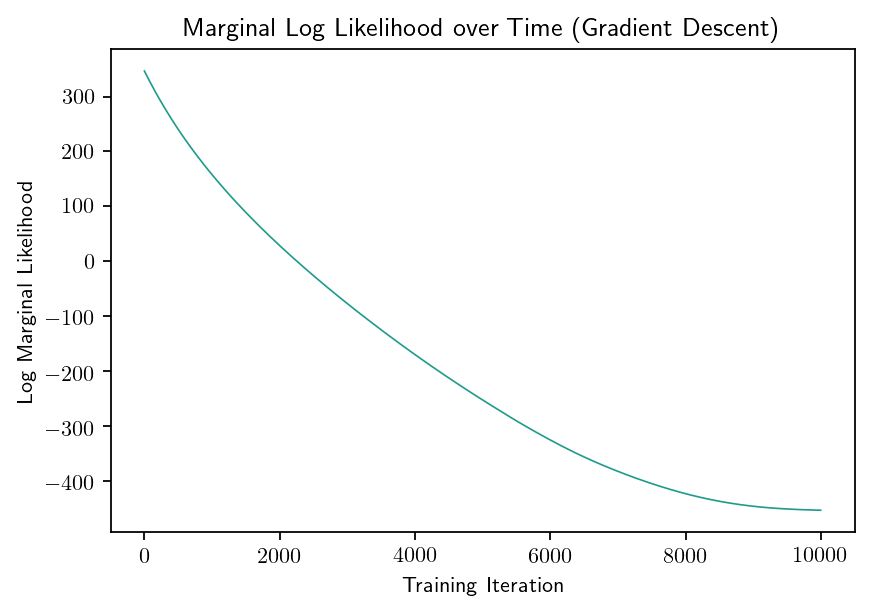
\includegraphics[width=1.0\textwidth]{img/gp/gp_likelihood.png}
	\caption{\textcolor{viridis5}{\textbf{Log-Likelihood}} of the prior kernel parameters during optimisation.}
	\label{fig:gp_likelihood}
\end{figure}

After $10.000$ iterations, the following set of parameters is found and denotes the point estimate $\hat{\theta}$ for this example slice. 

\begin{equation}
	\begin{split}
		\hat{\theta} = \{ & \\
		& \sigma_s = 0.021854665592977836, \quad \ell_s = 4.2588876554564825 \\
		& \sigma_p = 0.05387198576409192, \quad p_p = 0.49980015957564133 \\
		& \ell_p = 0.3679243361111636, \quad \sigma_{lp1} = 0.05387198576409192 \\
		& \ell_{lp1} = 0.8774408675206453, \quad p_{lp1} = 2.7182818284590446 \\
		& \sigma_{lp2} = 0.3678794411714424, \quad \ell_{lp2} = 0.37381285294546657 \\
		& \sigma_{rq} = 0.01416396988294803, \quad \alpha_{rq} = 0.6015559752066347 \\
		& \ell_{rq} = 4.146611585773073, \quad \sigma_{m1} = 0.004795200159066785 \\
		& \ell_{m1} = 1.832663754018536, \quad \sigma_{m3} = 0.3678794411714424 \\
		& \ell_{m3} = 0.3678794411714424, \quad \sigma_{m5} = 0.01162291185946003 \\
		& \ell_{m5} = 5.030183381753336, \quad \sigma_{noise} = 8.441068346451243 e^{-05} \\
		\} & \\
	\end{split}
\end{equation}

Using these, a $\mathcal{GP}$ is fitted to the available data points. Having the fitted $\mathcal{GP}$ available, 50 draws are being taken for the shown visualisations, which are illustrated in figure \ref{fig:gp_data_example_posterior_gradient_descent}. One drawing is printed in bold to visualise how a simulated slice will look like.

\begin{figure}[hbt]
	\center
	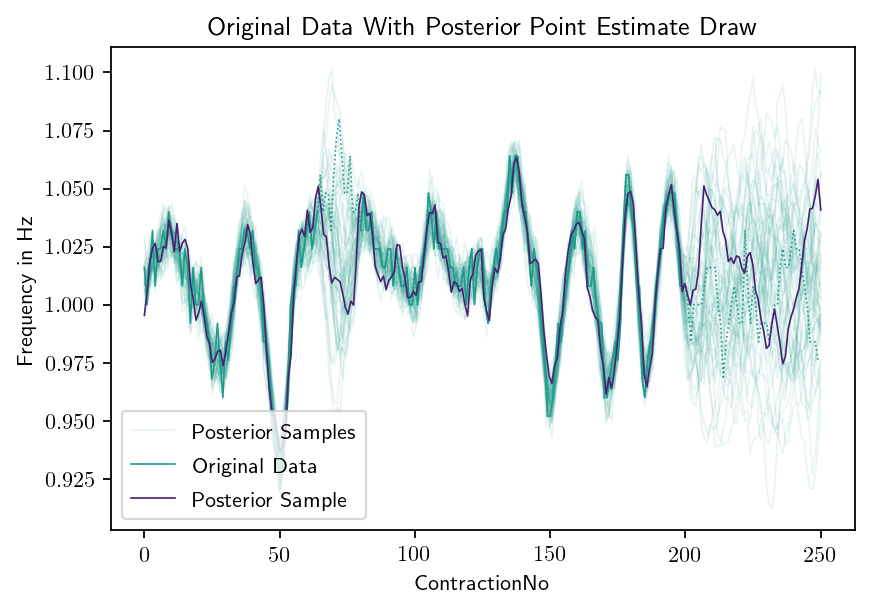
\includegraphics[width=1.0\textwidth]{img/gp/gp_data_example_posterior_gradient_descent.png}
	\caption{Draws from the \textcolor{viridis5}{\textbf{Gaussian Process}} with point estimates for the optimal parameters.}
	\label{fig:gp_data_example_posterior_gradient_descent}
\end{figure}

Figure \ref{fig:gp_data_example_posterior_intervals_gradient_descent} shows the mean of the $\mathcal{GP}$ together with its confidence bands and prediction bands. The variance at the indices of missing data is higher compared to the variance at known data. Both bands are quite similar in their uncertainty, as there is only one data point available for each point in time and point estimates do not account for the uncertainty in the parameters. Figure \ref{fig:gp_optimised_kernel_gradient_descent} shows the optimised kernel for this slice of data using gradient descent.

\begin{figure}[hbt]
	\center
	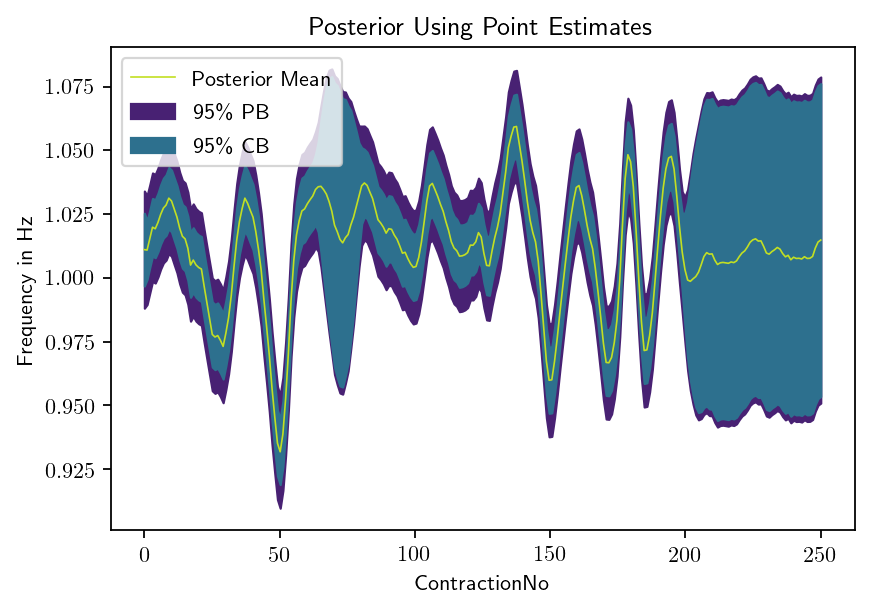
\includegraphics[width=1.0\textwidth]{img/gp/gp_data_example_posterior_intervals_gradient_descent.png}
	\caption{\textcolor{viridis9}{\textbf{Mean}} with \textcolor{viridis3}{\textbf{Confidence Bands}} and \textcolor{viridis0}{\textbf{Prediction Bands}} with points estimates for the optimal parameters.}
	\label{fig:gp_data_example_posterior_intervals_gradient_descent}
\end{figure}

 After careful consideration it has been decided that this approach will not be further investigated due to two reasons. Firstly, the fitting of $\hat{\theta}$ takes a lot of time. More precisely this means around 6 minutes for each slice, so having 96 slices for each time series and 181 series in total that results in $28$ days of computational time. Secondly, the point estimates do not account for the uncertainty in the parameters of the kernel, making the second approach of sampling from the posterior predictive distribution more attractive.

\begin{figure}[hbt]
	\center
	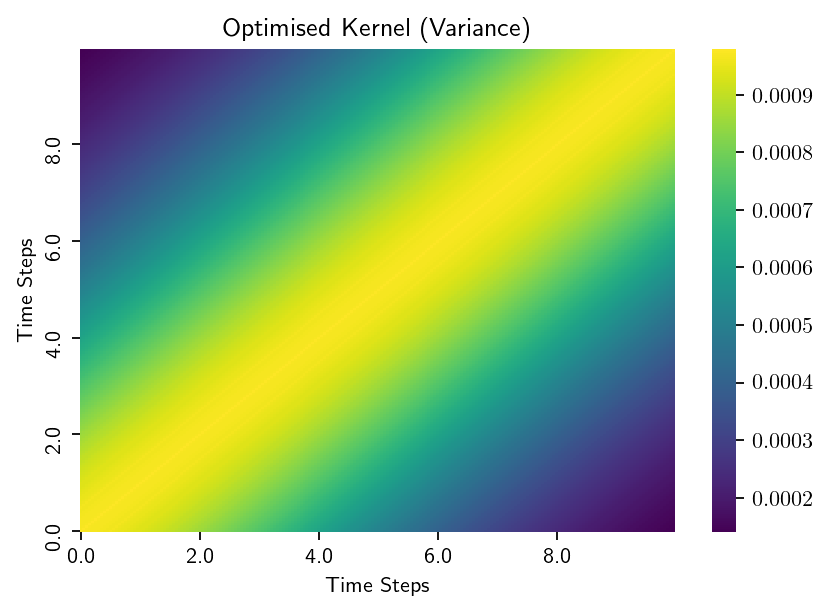
\includegraphics[width=1.0\textwidth]{img/gp/gp_optimised_kernel_gradient_descent.png}
	\caption{Optimised kernel using gradient descent.}
	\label{fig:gp_optimised_kernel_gradient_descent}
\end{figure}

\FloatBarrier
\subsubsection{Posterior Predictive Distribution}

The implementation uses TensorFlow Probability\footnote{\texttt{https://www.tensorflow.org/probability}}. The initial prior for all hyperparameters is given by:

\begin{equation}
	\text{Lognormal}(x, \mu = 0, \sigma = 1) = \frac{1}{x \sigma \sqrt{2\pi}} \exp \Bigg( - \frac{\big(\text{ln}(x) - \mu \big)^2}{2\sigma^2} \Bigg)
\end{equation}

This prior is considered uninformative in the given context and adds the property that the parameters are always positive (as length scale, period and variance are always positive). Hamiltonian Monte Carlo (HMC) [\cite{neal2012mcmc}] is used for sampling from the posterior according to the log marginal likelihood \ref{eq:gp_log_marginal_likelihood} of the $\mathcal{GP}$. The step size is initially 0.1 and adaptive, aiming for an acceptance probability of 0.75. A larger step size leads to faster progress but also increases the probability of rejecting a draw. The implementation is based on [\cite{hoffman2011nouturn}, chapter 3.2]. The number of leapfrog steps is set to 8 and defines how many steps the leapfrog integrator is ran. 10 chains run concurrently with 200 burn-in steps each and the noise variance is assumed to be 0. It takes around 50 seconds for fitting one slice. Having 181 time series with 96 slices each, the computational time for this approach is around 4 days and thus faster compared to the point estimate approach. 

\begin{figure}[hbt]
	\center
	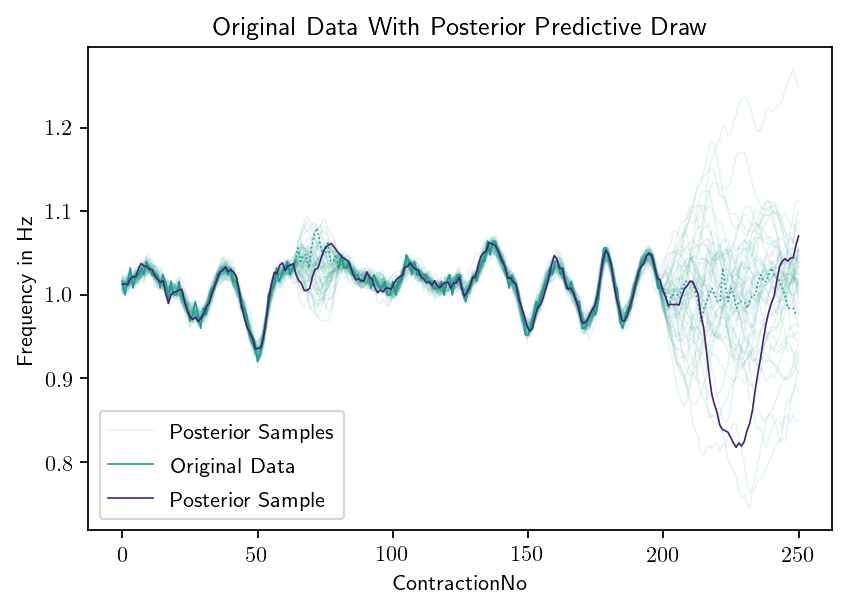
\includegraphics[width=1.0\textwidth]{img/gp/gp_data_example_posterior_predictive.png}
	\caption{Draws from the \textcolor{viridis5}{\textbf{Gaussian Process}} with posterior distributions for the parameters.}
	\label{fig:gp_data_example_posterior_predictive}
\end{figure}

Figure \ref{fig:gp_data_example_posterior_predictive} shows the example slice, where the original slice is denoted by a dashed line. Multiple posterior draws are shown with a slight green line, where one posterior draw is presented with a bold blue line. These posterior draws will be used as the new, simulated data. It can be seen that around contraction number 60, the uncertainty in the posterior draws is higher, as well as towards the end of the slice where the time series is padded.


\begin{figure}[hbt]
	\center
	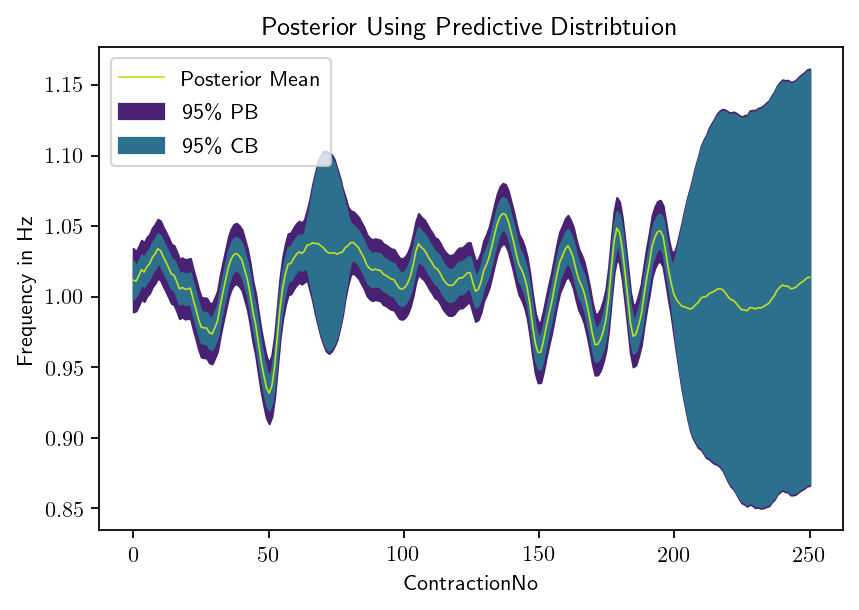
\includegraphics[width=1.0\textwidth]{img/gp/gp_data_example_posterior_intervals_predictive.png}
	\caption{\textcolor{viridis9}{\textbf{Mean}} with \textcolor{viridis3}{\textbf{Confidence Bands}} and \textcolor{viridis0}{\textbf{Prediction Bands}} with posterior distributions for the parameters.}
	\label{fig:gp_data_example_posterior_intervals_predictive}
\end{figure}

Figure \ref{fig:gp_data_example_posterior_intervals_predictive} shows the 95 per cent confidence and prediction interval together with the mean of the posterior draws. It can be seen that, due to the fact that we have just one data point for each point in time, the confidence and prediction bands are quite closely tight together. The increased uncertainty can be seen as well.


\begin{figure}[hbt]
	\centering
	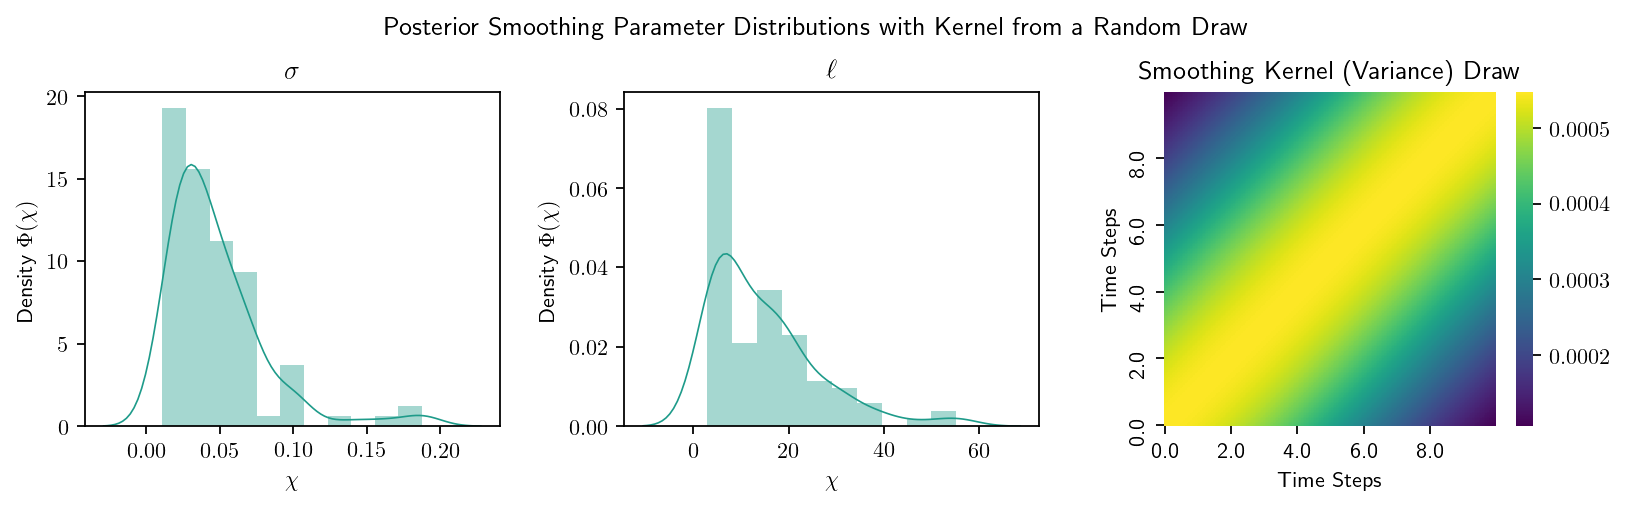
\includegraphics[width=1.2\textwidth,center]{img/gp/gp_kernel_posterior_smoothing_zoomed.png}
	\caption{\textcolor{viridis5}{\textbf{Posterior Distributions}} for the smoothing kernel with example draw for the kernel.}
	\label{fig:gp_kernel_posterior_smoothing}
\end{figure}

For one of the kernels, namely the smoothing kernel, the posterior parameter distributions are displayed in figure \ref{fig:gp_kernel_posterior_smoothing}. Note that the smoothed distribution includes areas below zero, but the histograms show that all draws are positive. The visualised kernel on the right-hand side represents the resulting kernel of one draw from the posterior distributions, thus the kernel actually changes for each draw. The distributions of all other hyperparameters and a respective kernel draws can be found in appendix \ref{sec:posterior_kernel_distributions_with_heatmaps}.

\clearpage
\FloatBarrier
\section{Results}

This results chapter is divided into three parts. In the first part, the results for the Gdańsk dataset are presented. The second part shows the results for the dataset from Physionet and the third part investigates the results for the data simulated based on the Gdańsk dataset. The baseline models always refers to the naive approach of always predicting the class which is represented most in the training dataset. For the Gdańsk dataset, with seven categories, the baseline is $18.23$ per cent and for the Physionet dataset, with six categories, the baseline is $39.14$ per cent.

\subsection{Gdańsk}

\begin{table}[h]
\caption{Accuracies of the feature-based models on the dataset provided by the University of Gdańsk. The baseline of always predicting the most represented class label in the training dataset is 18.23 per cent.}
    \label{tab:results_gdansk_feature}
\begin{adjustwidth}{-1in}{-1in}
    \centering
    \begin{tabular}{lrrrr}
    \multicolumn{5}{c}{\textbf{Gdańsk (Feature)}} \\
    \multicolumn{5}{c}{} \\
    \textbf{Accuracy} & \textbf{Naive Bayes} & \textbf{Random Forest} & \textbf{SVM} & \textbf{XGBoost} \\ \hline
        \multicolumn{5}{@{}l}{} \\
        \textbf{Regression / Complete} & \multicolumn{4}{@{}l}{}\\
        Training & & 45.14\% & 19.44\% & 28.47\%  \\ 
        Testing & & \textbf{37.83\%} & 29.73\% & 21.62\%  \\ \hline
        \multicolumn{5}{@{}l}{} \\
        \textbf{Regression / Constant} & \multicolumn{4}{@{}l}{}\\
        Training & & 24.31\% & 22.92\% & 22.22\% \\
        Testing & & 24.32\% & 27.02\% & 29.73\%  \\ \hline
        \multicolumn{5}{@{}l}{} \\
        \textbf{Classification / Complete} & \multicolumn{4}{@{}l}{}\\
        Training & 32.64\% & 73.61\% & 26.39\% & 68.06\%  \\
        Testing & 29.73\% & 24.32\% & 16.21\% & 21.62\%  \\ \hline
        \multicolumn{5}{@{}l}{} \\
        \textbf{Classification / Constant} & \multicolumn{4}{@{}l}{}\\
        Training & 21.53\% & 100.00\% & 34.72\% & 39.58\%  \\
        Testing & 27.03\% & \textbf{32.43\%} & 24.32\% & 24.32\% \\ \hline
    \end{tabular}
\end{adjustwidth}
\end{table}

Table \ref{tab:results_gdansk_feature} shows the results for the feature-based methods on the Gdańsk dataset. Most models perform better compared to the baseline, the only exception being the SVM conducting complete classification. The remaining models have an accuracy between 20 and 30 per cent. The three best performing models on the Gdańsk dataset are highlighted in bold, two of them are feature-based and hence found in table \ref{tab:results_gdansk_feature}. Overall, the best model combination consists of a Random Forest conducting constant classification and complete regression. It seems that the Random Forest had the tendency to overfit to the training dataset when conducting classification, still, cross-validation has found that this combination of methodology and model generalises best, which is fortified by the high test accuracies. The Naive Bayes classifier performs good considering its very short training time and very simplistic approach. While SVM and XGBoost, apart from one exception, perform above the baseline. It seems that they work better on the task of regression compared to classification. In summary, most feature-based models seem  to be able to beat the baseline. Nevertheless, due to the small test dataset with only 37 data points, the results are prone to fluctuation.

\begin{table}[h]
\caption{Accuracies of the DeepSleep-based models on the dataset providing by the University of Gdańsk. The baseline of always predicting the most represented class label in the training set is 18.23 per cent.}
    \label{tab:results_gdansk_deep}
\begin{adjustwidth}{-1in}{-1in}
    \centering
    \begin{tabular}{lrrr}
    \multicolumn{4}{c}{\textbf{Gdańsk (DeepSleep)}} \\
    \multicolumn{4}{c}{} \\
    \textbf{Accuracy} & \textbf{unweighted} & \textbf{weighted} & \textbf{oversampled}  \\ \hline
        \multicolumn{4}{@{}l}{} \\
        \textbf{Regression / Complete} & \multicolumn{3}{@{}l}{}\\
        Training & 13.89\% & & 18.52\%  \\ 
        Validation & 11.11\% & & 8.33\% \\
        Testing & 29.73\% & & 16.22\%  \\ \hline
        \multicolumn{4}{@{}l}{} \\
        \textbf{Regression / Constant} & \multicolumn{3}{@{}l}{}\\
        Training & 16.67\% & & 14.81\% \\
        Validation & 16.67\% & & 11.11\% \\
        Testing & \textbf{32.43}\% & & 18.92\%  \\ \hline
        \multicolumn{4}{@{}l}{} \\
        \textbf{Classification / Complete} & \multicolumn{3}{@{}l}{}\\
        Training & 23.19\% & 22.22\% & 35.19\%  \\
        Validation & 11.11\% & 13.89\% & 16.67\% \\
        Testing & 10.81\% & 10.81\% & 16.22\%  \\ \hline
        \multicolumn{4}{@{}l}{} \\
        \textbf{Classification / Constant} & \multicolumn{3}{@{}l}{}\\
        Training & 22.22\% & 13.89\% & 23.15\%  \\
        Validation & 13.89\% & 11.11\% & 19.44\% \\
        Testing & 10.81\% & 5.41\% & 13.51\% \\ \hline
    \end{tabular}
\end{adjustwidth}
\end{table}

The results for the DeepSleep model can be found in table \ref{tab:results_gdansk_deep}. DeepSleep seems to perform better when applying regression. The model working on the raw, unweighted data works best and yields in an overall accuracy of 32.43 per cent, which is the third-best model on this dataset. For the task of classification, independently of the methodology, the DeepSleep-based model performs worse than the baseline. When oversampling the data, the accuracies for classification increase, but still remain below the baseline accuracy. For DeepSleep-based models performing regression, the accuracies decrease when oversampling the data. Generally, it can be seen that the DeepSleep-based models performs worse compared to the feature-based methods on the Gdańsk dataset.

\begin{figure}[hbt]
	\center
	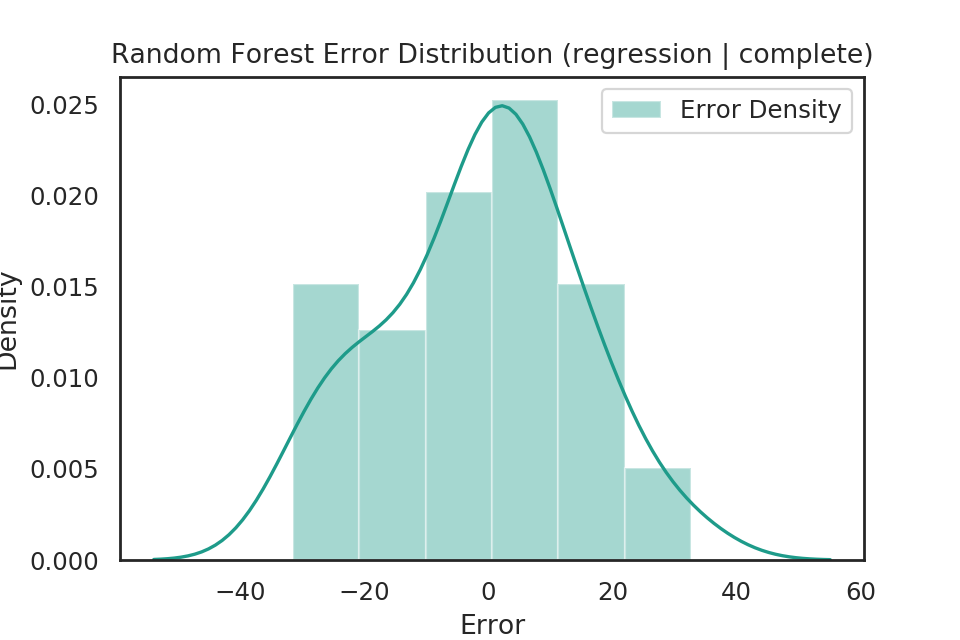
\includegraphics[width=1.0\textwidth]{img/learning/original_gdansk_random_forest_regression_complete_error_distribution.png}
	\caption{\textcolor{viridis5}{\textbf{Error distribution}} for Random Forest performing complete regression.}
	\label{fig:original_gdansk_random_forest_regression_complete_error_distribution_unbiased_inline}
\end{figure}

Figure \ref{fig:original_gdansk_random_forest_regression_complete_error_distribution_unbiased_inline} shows the error distribution for the Random Forest performing complete regression. It can be seen that it is almost normal distributed with a mean close to 0. The variance is high, yielding in a 95 per cent prediction band spanning between $-30.11$ and $30.11$, which is the whole age range included in the data. Nevertheless, the distribution does not show a misclassification that lies further away than 30 years from its real label. The Random Forest chosen by cross-validation consists of just 5 estimators, although having a depth of 30 splits.

\FloatBarrier
\subsection{Physionet}

\begin{table}[h]
\caption{Accuracies of the feature-based models on the dataset provided by Physionet. The baseline of always predicting the most represented class label in the training dataset is 39.14 per cent.}
    \label{tab:results_physionet_feature}
	\begin{adjustwidth}{-1in}{-1in}
    \centering
    \begin{tabular}{lrrrr}
    \multicolumn{5}{c}{\textbf{Physionet (Feature)}} \\
    \multicolumn{5}{c}{} \\
    \textbf{Accuracy} & \textbf{Naive Bayes} & \textbf{Random Forest} & \textbf{SVM} & \textbf{XGBoost} \\ \hline
        \multicolumn{5}{@{}l}{} \\
        \textbf{Regression / Complete} & \multicolumn{4}{@{}l}{}\\
        Training & & 60.45\% & 40.13\% & 42.44\% \\ 
        Testing & & 36.13\% & 30.32\% & 32.26\% \\ \hline
        \multicolumn{5}{@{}l}{} \\
        \textbf{Regression / Constant} & \multicolumn{4}{@{}l}{}\\
        Training & & 46.53\% & 40.26\% & 44.93\% \\
        Testing & & 30.59\% & 29.29\% & 30.45\% \\ \hline
        \multicolumn{5}{@{}l}{} \\
        \textbf{Classification / Complete} & \multicolumn{4}{@{}l}{}\\
        Training & 15.35\% & 99.78\% & 28.53\% & 46.33\% \\
        Testing & 12.90\% & 29.03\% & 25.81\% & 34.84\% \\ \hline
        \multicolumn{5}{@{}l}{} \\
        \textbf{Classification / Constant} & \multicolumn{4}{@{}l}{}\\
        Training & 13.46\% & 71.80\% & 32.05\% & 53.89\% \\
        Testing & 12.39\% & 33.94\% & 24.65\% & 33.81\% \\ \hline
    \end{tabular}
\end{adjustwidth}
\end{table}

The results for the feature-based models on the Physionet dataset are shown in table \ref{tab:results_physionet_feature}. None of the models managed to reach a higher accuracy than the baseline with $39.14$ per cent. The Naive Bayes classifiers result in very low accuracies, despite considering the prior class probabilities. Furthermore, tree-based models, like Random Forest and XGBoost, seem to perform best, although the SVM provides still quite reasonable performance. The same behaviour of seeing overfitted models generalising best can be observed again. Nevertheless, these overfitted tree-based models show the best results on the test dataset.

\begin{table}[h]
\caption{Accuracies of the DeepSleep-based models on the dataset provided by Physionet. The baseline of always predicting the most represented class label in the training dataset is 39.14 per cent.}
    \label{tab:results_physionet_deep}
\begin{adjustwidth}{-1in}{-1in}
    \centering
    \begin{tabular}{lrrr}
    \multicolumn{4}{c}{\textbf{Physionet (DeepSleep)}} \\
    \multicolumn{4}{c}{} \\
    \textbf{Accuracy} & \textbf{unweighted} & \textbf{weighted} & \textbf{oversampled}  \\ \hline
        \multicolumn{4}{@{}l}{} \\
        \textbf{Regression / Complete} & \multicolumn{3}{@{}l}{}\\
        Training & 24.07\% & & 27.63\% \\ 
        Validation & 28.57\% & & 25.32\% \\
        Testing & 25.16\% & & 31.61\% \\ \hline
        \multicolumn{4}{@{}l}{} \\
        \textbf{Regression / Constant} & \multicolumn{3}{@{}l}{}\\
        Training & 38.82\% & & 36.39\% \\
        Validation & 43.51\% & & 38.96\% \\
        Testing & 33.55\% & & 34.84\% \\ \hline
        \multicolumn{4}{@{}l}{} \\
        \textbf{Classification / Complete} & \multicolumn{3}{@{}l}{}\\
        Training & 39.47\% & 40.19\% & 29.01\% \\
        Validation & 37.66\% & 33.77\% & 25.32\% \\
        Testing & 38.06\% & 34.39\% & 23.87\% \\ \hline
        \multicolumn{4}{@{}l}{} \\
        \textbf{Classification / Constant} & \multicolumn{3}{@{}l}{}\\
        Training & 39.38\% & 21.23\% & 18.64\%  \\
        Validation & 33.77\% & 17.53\% & 19.48\% \\
        Testing & \textbf{42.58}\% & 16.13\% & 16.13\% \\ \hline
    \end{tabular}
\end{adjustwidth}
\end{table}

Looking at the results for the DeepSleep-based models in table \ref{tab:results_physionet_deep}, only the DeepSleep-based model conducting constant classification generalises and outperforms the baseline. Using a weighted loss for classification does not seem to help for age classification, yielding in low accuracies for constant classification. Also, oversampling the training data does not seem to improve the accuracies.

\begin{figure}[!hbt]
    \makebox[\linewidth][c]{
	\centering
	\subfigure[Loss]{\label{fig:original_physionet_sleepnet_classification_constant_none_unweighted_loss_inline}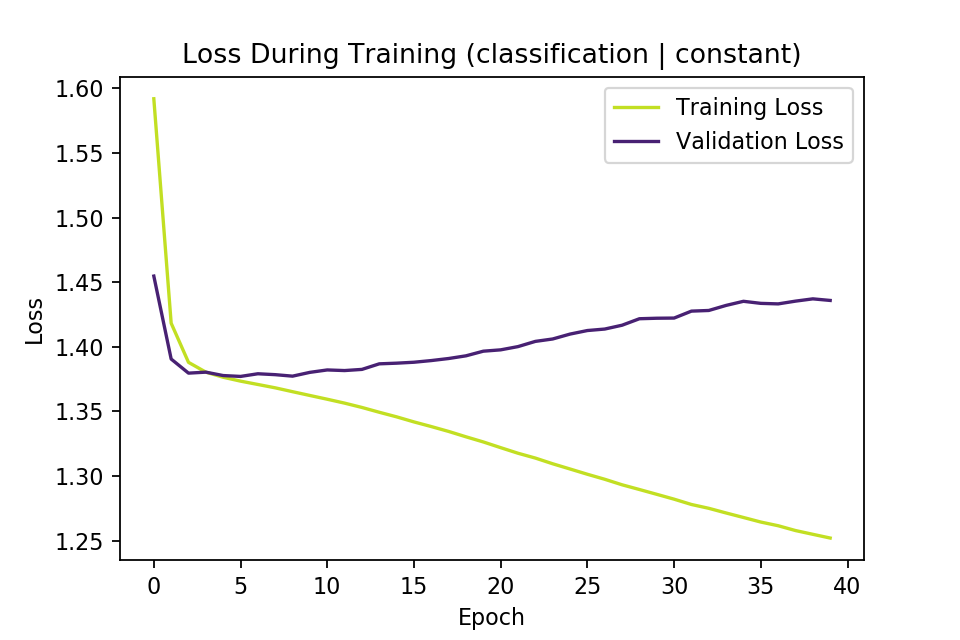
\includegraphics[width=0.6\textwidth]{img/learning/original_physionet_sleepnet_classification_constant_none_unweighted_loss.png}}
	\subfigure[Accuracy]{\label{fig:original_physionet_sleepnet_classification_constant_none_unweighted_accuracy_inline}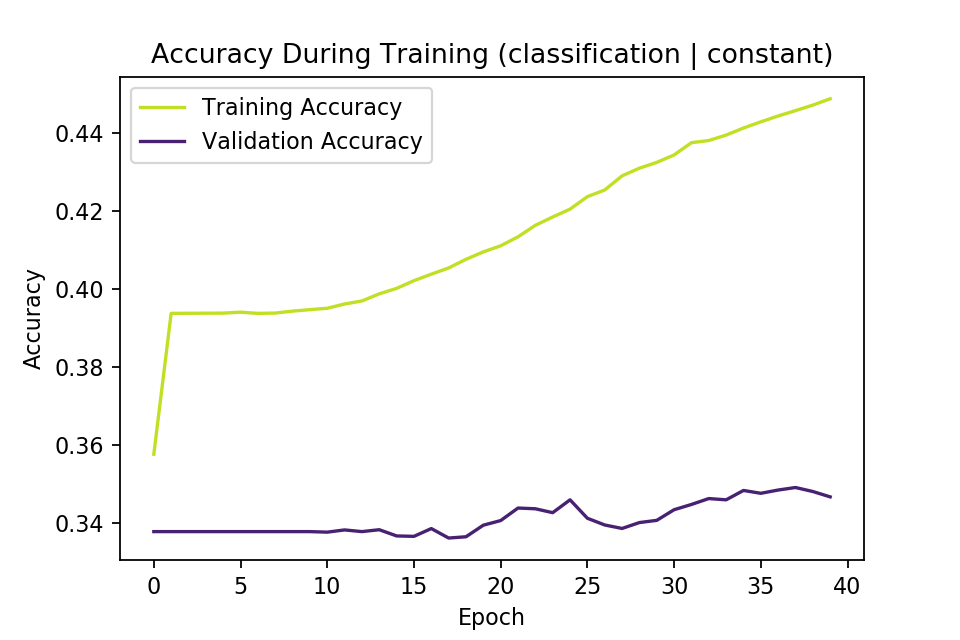
\includegraphics[width=0.6\textwidth]{img/learning/original_physionet_sleepnet_classification_constant_none_unweighted_accuracy.png}}
	}
	\caption{\textcolor{viridis9}{\textbf{Training}} and \textcolor{viridis0}{\textbf{validation}} loss and accuracy for DeepSleep performing standard constant classification.}
\end{figure}

Figure \ref{fig:original_physionet_sleepnet_classification_constant_none_unweighted_loss_inline} and \ref{fig:original_physionet_sleepnet_classification_constant_none_unweighted_accuracy_inline} show the learning curves for cross-entropy loss and accuracy during training of DeepSleep-based model performing constant classification. Note that the accuracy score during training is evaluated differently compared to the reported final predictions. During training, a label is considered correct, if it lies within a range of five years of the true label. The final prediction will automatically choose the lowest or highest label, even if the prediction lies further away. For example, during training, a prediction of 91 would be considered as wrong, whereas during the final classification the highest label, here from 80-90, would be chosen. The reason for this difference in accuracy evaluation enables to monitor the accuracy more precisely during training and to achieve better results during prediction. Also, the accuracy reported on the training dataset during the training of the model is evaluated while the model has dropout enabled. For the finally reported accuracy scores for all datasets, dropout is disabled. Analysing these plots, it can be noticed that both loss curves are dropping quickly at the beginning. While the training loss continues to decrease, the validation loss starts growing again.

Overall, the model with the lowest validation loss is chosen by early stopping. Due to the larger size of the Physionet dataset, less epochs are required for a convergence of the model. This effect is even more noticeable on the oversampled dataset, where the validation accuracy shows that the model barely learns new information. Even though the accuracy increases towards the end of the training, the validation loss continuously becomes worse.

\FloatBarrier
\subsection{Simulated Dataset}

Table \ref{tab:results_simulated_data} shows the results for the different models ran on the simulated dataset.

\begin{table}[h]
\caption{Accuracies of all models except Naive Bayes on the simulated dataset. The baseline of always predicting the most represented class label in the training dataset is 18.23.}
    \label{tab:results_simulated_data}
\begin{adjustwidth}{-1in}{-1in}
    \centering
    \begin{tabular}{lrr}
    \multicolumn{3}{c}{\textbf{Simulated Dataset}} \\
    \multicolumn{3}{c}{} \\
    \textbf{Accuracy} & \textbf{Regression / Constant} & \textbf{Classification / Constant} \\ \hline
        \multicolumn{3}{@{}l}{} \\
        \textbf{Random Forest} & \multicolumn{2}{@{}l}{}\\
        Training & 59.89\% & 99.99\% \\ 
        Testing & 21.82\% & 21.24\% \\ \hline
        \multicolumn{3}{@{}l}{} \\
        \textbf{Support Vector Machine} & \multicolumn{2}{@{}l}{}\\
        Training & 23.90\% & 33.28\% \\
        Testing & \textbf{31.16\%} & 15.46\% \\ \hline
        \multicolumn{3}{@{}l}{} \\
        \textbf{XGBoost} & \multicolumn{2}{@{}l}{}\\
        Training & 37.79\% & 99.04\% \\
        Testing & 22.05\% & 23.94\% \\ \hline
        \multicolumn{3}{@{}l}{} \\
        \textbf{DeepSleep} & \multicolumn{2}{@{}l}{}\\
        Training & 20.94\% & 29.75\% \\
        Validation & 18.01\% & 25.43\% \\
        Testing & \textbf{27.66\%} & 13.08\% \\ \hline
        \multicolumn{3}{@{}l}{} \\
        \textbf{DeepSleep (weighted)} & \multicolumn{2}{@{}l}{}\\
        Training & & 29.26\% \\
        Validation & & 31.33\% \\
        Testing & & 19.41\% \\ \hline
        \multicolumn{3}{@{}l}{} \\
        \textbf{DeepSleep (oversample)} & \multicolumn{2}{@{}l}{}\\
        Training & 23.43\% & 30.75\% \\
        Validation & 15.24\% & 26.42\% \\
        Testing & \textbf{29.51\%} & 17.65\% \\ \hline
    \end{tabular}
\end{adjustwidth}
\end{table}

It can be seen that the achieved accuracies for the simulated dataset are not higher compared to the original Gdańsk dataset. The models that performed below the baseline are the SVM conducting classification, the DeepSleep-based model conducting classification as well as the DeepSleep-based model running on oversampled data and conducting classification. For almost all models, the accuracies are higher when performing regression. The three highest test accuracies for the simulated dataset are marked in bold. Despite that fact that these three models still have a smaller accuracy than the best performing models on the Gdańsk dataset, the results seem to be more stable with less outliers in terms of very low accuracies.\footnote{All metrics for the different models can be found in the appendix.}

Even though an epoch of the DeepSleep-based model has a longer running time than the the epochs in the other models for the simulated data, it still results in an overall lower training time. This is due to the fact that less training epochs are needed while still achieving roughly the same results.

In regions of high variance, the data simulation, based on Gaussian processes, can sample negative values. Naive Bayes cannot handle these values, as it assumes them to be frequencies which are not allowed to be negative by definition. As the simulation returned at least one negative value, Naive Bayes is not included in the results for the simulated data.

\clearpage
\section{Discussion}

This chapter will analyse and discuss the results presented in the previous chapter, with the aim to answer the originally defined research questions. Also, the limitations of the different approaches, along with the data, will be discussed. To put the results into perspective, we will compare them with [\cite{threeclassclassification}] and [\cite{patternshrd}].

\subsection{Applicability of Cardiovascular Age Prediction}

Comparing the results from both datasets, it seems that the models extract more information when working on the Gdańsk dataset. That follows from the difference between the best and average accuracies of the models compared to the baselines. This can be due to several reasons, though it can not be assessed which one is the actual cause. One reason could be, that the Gdańsk dataset only includes healthy patients which encodes more information about cardiovascular age. Furthermore, the dataset is close to balance compared to the dataset from Physionet. Another possible reason is, that it is easier to predict the cardiovascular age, if the RR intervals during nocturnal sleep are given. As the Physionet dataset provides recordings throughout the whole day, this could add impurity or noise to the information embedded in the nocturnal sleep stages. Additionally, it could be that the given cardiovascular diseases in the Physionet dataset have such a high impact on the models, that the embedded information about age becomes prone to the changes implied by those diseases. Further investigations would be necessary to evaluate the actual cause for the different predictable strengths of the models. Another takeaway is, that the original assumption, that regression provides more information for the model and thus provides better results, does not hold for the feature-based models. However, the DeepSleep-based model, based on gradient descent, seems to completely fail to learn on the task of classification and benefits from defining the problem as a regression problem.

When comparing the error distributions of the different models and methodologies, it can be seen that the error distributions do not differ much from each other, thus the variance seems to be roughly the same, also when comparing the distributions of both datasets with each other. This strengthens the choice of evaluating two datasets, as it seems that the underlying uncertainty remains the same, regardless of the chosen model methodology or dataset. Ignoring the fact that all these combinations represent just a sample from the real world. Inferentially, it can be that accurately predicting the cardiovascular age to a certain degree, only given the RR intervals of a subject, might not be possible. This statement still implies, that if the number of classes is considerable low (speaking of two or three), the different models and methodologies might be accurate enough to serve their purpose. Overall, that is dependent on which objectives the models are supposed to support. For the original research question, if these models can accurately predict the cardiovascular age within a range of ten years (thus age decades), the answer is, that they can not.

This leaves us with the comparison of the obtained results with other papers to ensure that we can be certain about the obtained results. Therefore, we will investigate and compare the obtained results of [\cite{threeclassclassification}] and [\cite{patternshrd}]. In [\cite{threeclassclassification}], 60 subjects, 20 for each age group (18-30, 30-45, 45-60), were classified with a maximum accuracy of 70 per cent. The obtained accuracy is quite high, but accounting for the larger age range as well as the lower amount of classes, this is in accordance with the obtained error distributions from this thesis. Moreover, out of these 60 subjects, 30 have been used for training and 30 for testing, thus representing just a small sample. [\cite{patternshrd}] conduct a more thorough analysis of the problem: The reported \textit{very high} accuracies of around 96 per cent are for the training set only, as no validation or test set has been used. This becomes evident when investigating figure 8 in the paper, where the reported results are clearly stated for the whole dataset (the Gdańsk dataset), with 181 subjects and respective subsets for the different age decades, always covering all samples. This implies that the reported accuracies are training accuracies and might be severely overfitted to the training data. Delving deeper into their results, chapter 3.4 states that they used a SVM with a Gaussian kernel, where $\gamma = 0.2$ and $C=1.0$. A high value of C enforces the SVM to choose the smallest error margins possible, trying to prevent outliers at all cost. This does not necessarily mean that a SVM with a high C overfits to its training data per se, but makes it more likely, as the decision boundary is more flexible to account for the training points. If we compare their value of C with the ones that we found using cross-validation, this problem becomes more eminent: $C = [0.3, 0.5, 0.5, 1.0, 0.6, 0.1, 0.5, 0.1]$. Out of 8 differently trained SVM models, only one chose $C=1.0$, all of the others clearly chose lower values for C. The model that chose $C=1.0$ is the SVM conducting constant classification on the Gdańsk dataset, with a test accuracy of 24.34 per cent. Additionally, the used metrics for validation, which consists of shuffling the time series, is questionable, especially as a simple method as hold-out data could have been used. We conclude from that, that the reported results provided by [\cite{patternshrd}] do not allow for any conclusions about the generalisation of their reported models. Taking the results from both papers into account, the obtained results seem to be reasonable.

The simulation of the data requires a lot of computational resources. The intention was to provide the models with more various data and thereby support the model to generalise better, which ultimately should yield in better results. The results for the models, ran on the simulated data, do not provide better accuracies, but seem to solve the problem that some methodologies resulted in accuracies way below the baseline. As already stated, the DeepSleep model takes less epochs and therefore also less time to train. Nevertheless, this does not seem to be worth the time required for simulating the data. It indeed seems that the effort of complex data simulation does not provide better results, at least for this problem. Considering that the accuracies are quite low in general, the room for improvements is small.

\subsection{Theoretical Analysis}

One interesting observation is that some feature-based models that have been selected by cross-validation seem to have a large gap between training and test accuracy. This applies specifically to the tree-based methods Random Forest and XGBoost. This finding is especially unusual for XGBoost as it, in addition to cross-validation, also uses regularisation as can be seen in equation \ref{eq:xgboost_regularisation}. Considering this, there are to matter to think about. Firstly, do these models overfit? That depends foremost on the definition of an overfitted model. Is a model that generalises best compared to other models, but still has a large difference in train and test accuracy, considered overfitted? The answer most likely depends. As none of the models achieved a high accuracy, we can safely conclude that these models most likely overfitted, despite having the best set of hyperparameters determined by cross-validation.

Inspecting loss and accuracy of the DeepSleep based model performing complete classification on the Gdańsk dataset in figure \ref{fig:original_gdansk_sleepnet_classification_complete_none_unweighted_loss} and figure \ref{fig:original_gdansk_sleepnet_classification_complete_none_unweighted_accuracy} respectively, it can be observed that the loss immediately becomes worse with the second epoch while the accuracy remains roughly the same throughout the training of the model. Looking at the loss in figure \ref{fig:original_gdansk_sleepnet_classification_constant_none_weighted_loss} and the corresponding accuracy in figure \ref{fig:original_gdansk_sleepnet_classification_constant_none_weighted_accuracy} for the same model again conducting weighted, constant classification, it can be seen that the loss becomes worse as well but this time the accuracy seems so slightly increase each epoch. This is an odd finding and raises the question, if the loss function, in this case, cross-entropy, is appropriate as the accuracy becomes better while the loss becomes worse. If we assume the problem to be a regression, for example in figure \ref{fig:original_gdansk_sleepnet_regression_constant_oversample_loss} which shows the loss and figure \ref{fig:original_gdansk_sleepnet_regression_constant_oversample_accuracy} the accuracy, the curves make more sense. One things which remains interesting is the \textit{plateau} around epoch 60 where the loss and the lowest and the accuracy the highest. In this setting, the loss function actually represents the accuracy well. The DeepSleep based model seems to perform better for a regression loss and the behaviour seems to be more natural. Nevertheless, this does not yet explain why this is not the case for the feature-based models.

It seems that choosing an LSTM does not only enable the model to learn long-term dependencies, but also enforces the usage of a loss that accurately represents the embedded information on a continuous spectrum. It might be of interest to investigate this further, based on an easier task such that is easier to track which settings cause which behaviour. In the current setting, it is not possible to spot the unique cause of the observed behaviours.

\subsection{Deep Learning in Perspective}

Opting for deep learning models is not always the correct path to follow, as they do not necessarily provide better results. On the other hand, feature-based models have the problem, that they do not scale well. Especially SVMs require a lot of training time, as they involve solving a quadratic programming problem, which adds constraints to an equation to solve. Also taking hyperparameter search and prediction into account, feature-based methods can be very slow. All feature-based models in this thesis were run only on a small subset of the available data, withholding some of the information that would be available for the models. Deep learning models themselves also take their time for fitting, but usually deep learning models scale quite well in a way that they can be parallelised on GPUs, resulting in lower run times. It is not very common to do extensive grid hyperparameter search for deep learning models, hence some time must be spent on choosing the right hyperparameters as well as the right model architecture. Contrary to deep learning approaches, feature-based models require manually constructed features, which are not that straight forward to construct for time series data. In the end, the models to choose always depend on the problem.

\subsection{Result Evaluation}

We know from other sources, that there is some information embedded in the RR signals, which includes disease or nocturnal sleep detection. However, it seems like the age of a person is not embedded into the signal. The DeepSleep model is rather complex, still, it does not perform better compared to the simple feature-based models. Usually, complex deep learning models accomplish at least the same level of results for a given problem set, which is not the case here. Also, considering that weighting the classes, as well as oversampling the training dataset, yields in worse results, the question is raised, if the models that achieved high accuracies actually generalised or if they simply learned the class distribution. For some feature-based models, grid search for the hyperparameters as well as cross-validation, resulted in over 2,000 models fitted. With this high amount of fits, it could have quite likely happened that one of the higher test accuracies just happened by chance for the Gdańsk dataset, as the test dataset is rather small. Considering the results from the second datasets, where more data is available, this assumption could be quite likely, as there are no models that achieved a significantly higher accuracy compared to the baseline. Unfortunately, there is no simple way of proofing this assumption.

It is hard to confidently explain these low accuracies. Given all these different methodologies and models, it is quite unlikely that one mistake holds for all of these different approaches. Especially, as the obtained results are consistent with results provided by other papers. Therefore, it seems unlikely that a discrepancy remains uncovered. We conclude from this, that the desired information is just not available in RR intervals. Assuming this hypothesis to be true, it raises the questions if there is another way of improving the results. One way could be to simply provide more information to the models. The original problem was to be able to label data in the medical field, where the quality of the data is not assumed to be good. Presumably, we do not expect a lot more meta-information about the subjects. Nevertheless, what might be available is not the RR intervals, but the raw underlying data as it is shown in figure \ref{fig:rr_interval}. If that is the case, further analysis could be conducted on this data to see if that improves the results. Having a better resolution on the labels available could potentially help the models to extract more information as the current labels are quite blurry as they span a time range of ten years.

Considering all this, the true purpose of labelling new data should not be forgotten. Hospitals have unlabelled data, so when automating the labelling, a high accuracy should be ensured, since the data will most likely be, especially considering that this data will most likely be used for clinical research and erroneous labelled data could have severe impacts. It is up for debate, which accuracy or error distribution would be acceptable, but no matter how it would be defined, the results obtained in this thesis indicate, that they are still far from being applicable in a practical context. Even if one manages to increase the accuracies to 80 per cent for the given datasets, it is questionable if that would be enough for applying these models in the required context.

Concludingly, the results of this thesis show, that the accuracies for cardiovascular age prediction are not yet sufficient for any real-world application. 

\clearpage
\section{Conclusion}

The main takeaway from this thesis is, that cardiovascular age prediction, based on RR intervals is a difficult problem. We have seen other research indicating high accuracies, which themselves do not provide a good estimate for how well a model generalises. The aim of developing models should always be, to make them generalise to unseen data. To get an estimate of its general predictive strength, at least held-out data should be used. A better estimate could be obtained when the actual test data is coming from a different context, to prevent a bias towards the given dataset. Therefore, to create a model which performs well on various types of RR intervals, one should also train this model on different sources of RR intervals. This can for example include recordings of people doing sports, sleeping or having diseases. However, acquiring a dataset that embeds all of this information, is a challenging task in itself.

We can also conclude, that for time series processing, linear spline interpolation works rather well compared to other methods, especially considering how simple this approach of handling impurity is. It remains unsolved to which extend this applies to other time series data. Considering the low accuracies obtained, it is also hard to tell how good $\mathcal{GP}$s would work in a context where the desired information is easier accessible for the models. Still, $\mathcal{GP}$s have the benefit of providing a distribution for sampling as well as the ability to be evaluated at any predictive point. In the end, they add variability to the existing data, but are unfortunately limited to smaller slices due to their computational complexity. In a Bayesian setting, some information can flow between the slices. Ultimately, it would be of interest to consider the complete time series as well as all of them at the same time for fitting the $\mathcal{GP}$. At the moment, this is computationally infeasible, but frameworks such as TensorFlow Probability enable GPU acceleration and thus provide a possibility to use these kinds of methods within new fields.

To continue the work on this task of age prediction, the most promising directions are to either gather more relevant meta-information or more detailed time series including QQ-intervals or the raw input signal of an ECG. Also, constructing new features could be a way to improve the existing models rather than trying to tweak the existing complex models.

\clearpage

%%% BIBLIOGRAPHY

\addtocontents{toc}{\protect\setcounter{tocdepth}{3}}
\clearpage
\section{References}
\printbibliography[heading=none]

\clearpage

\addtocontents{toc}{\protect\setcounter{tocdepth}{2}}
\section{Appendix}
\label{sec:appendix}

The appendix includes information about the Bayesian data simulation as well as all metrics and hyperparameters associated to all models found in this thesis.

\subsection{Posterior Kernel Distributions with Heatmaps}
\label{sec:posterior_kernel_distributions_with_heatmaps}

\begin{figure}[!hbt]
	\center
	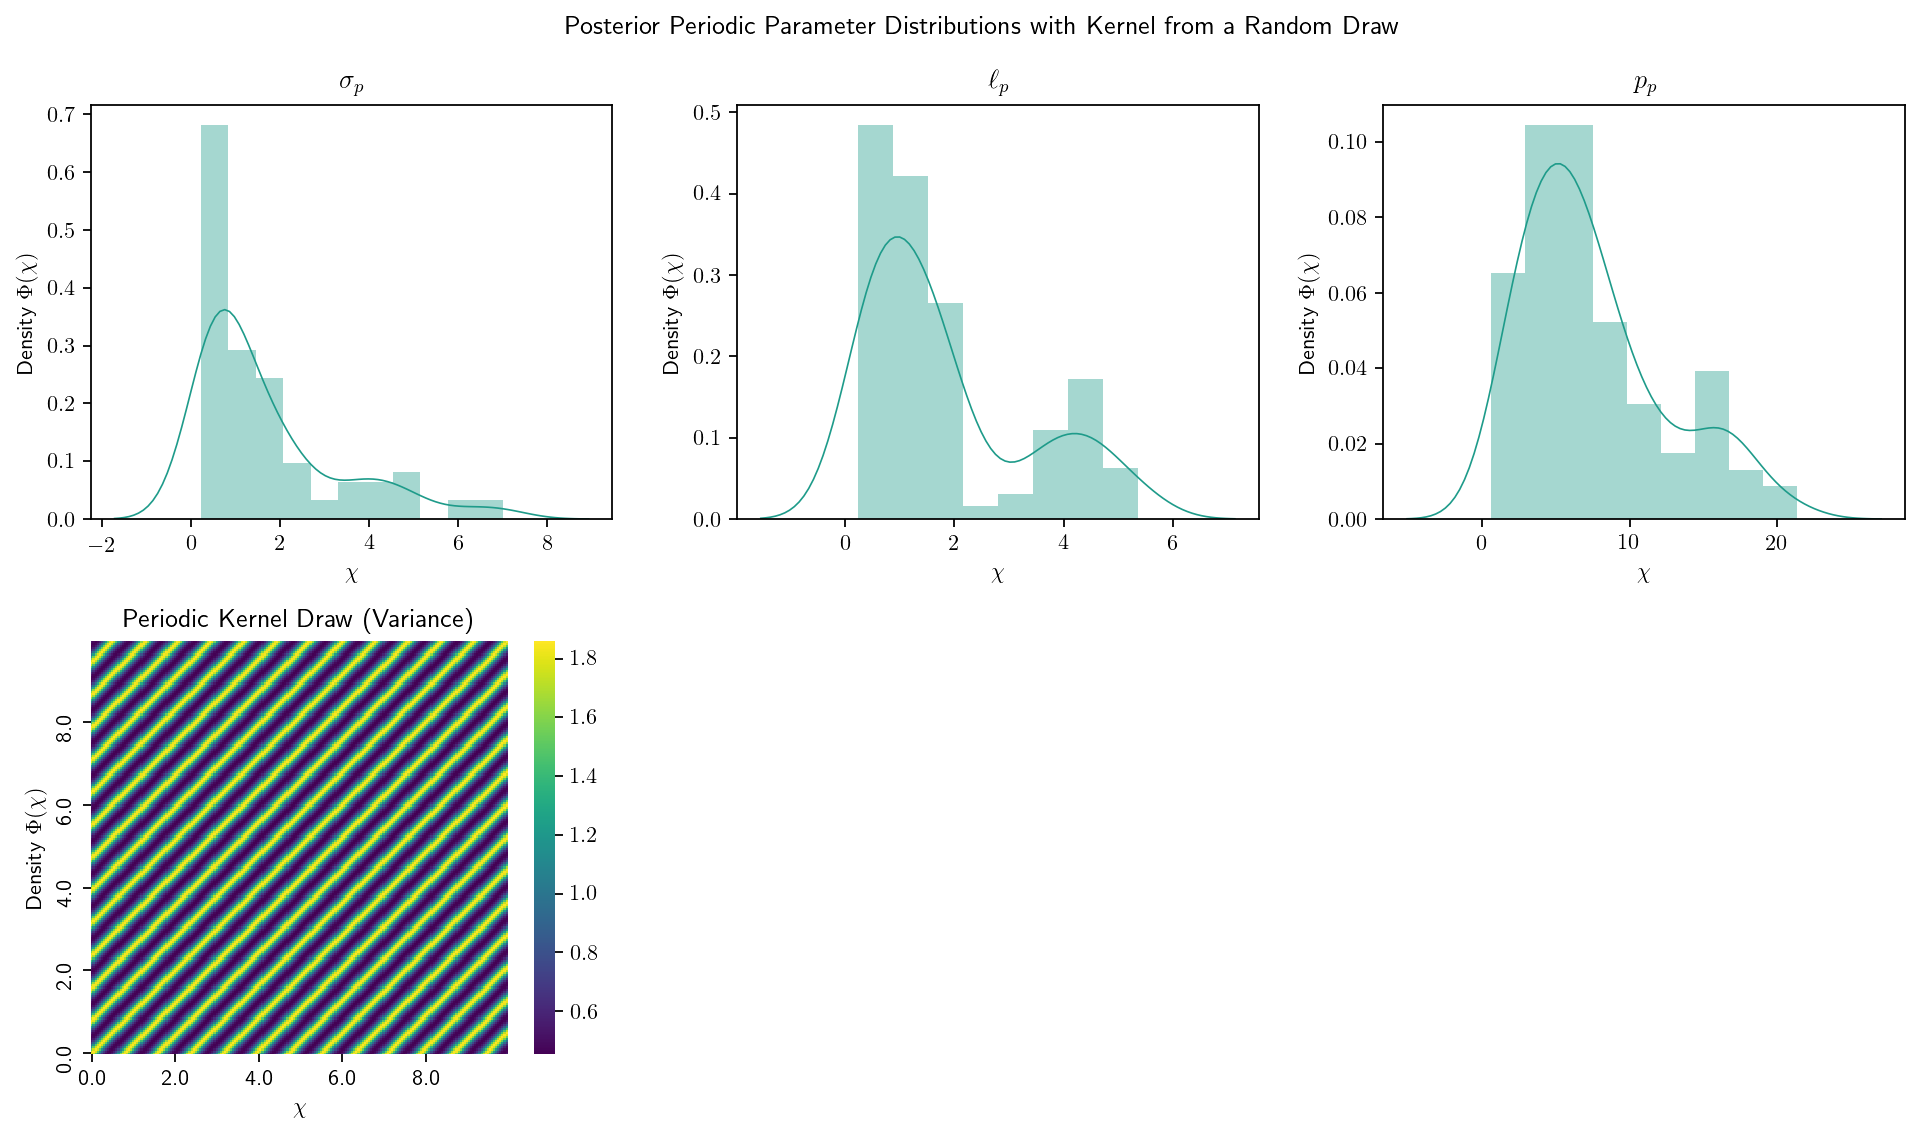
\includegraphics[width=1.2\textwidth,center]{img/gp/gp_kernel_posterior_periodic_zoomed.png}
	\caption{\textcolor{viridis5}{\textbf{Posterior Distributions}} for the periodic kernel with example draw for the kernel.}
	\label{fig:gp_kernel_posterior_periodic}
\end{figure}

\begin{figure}[!hbt]
	\center
	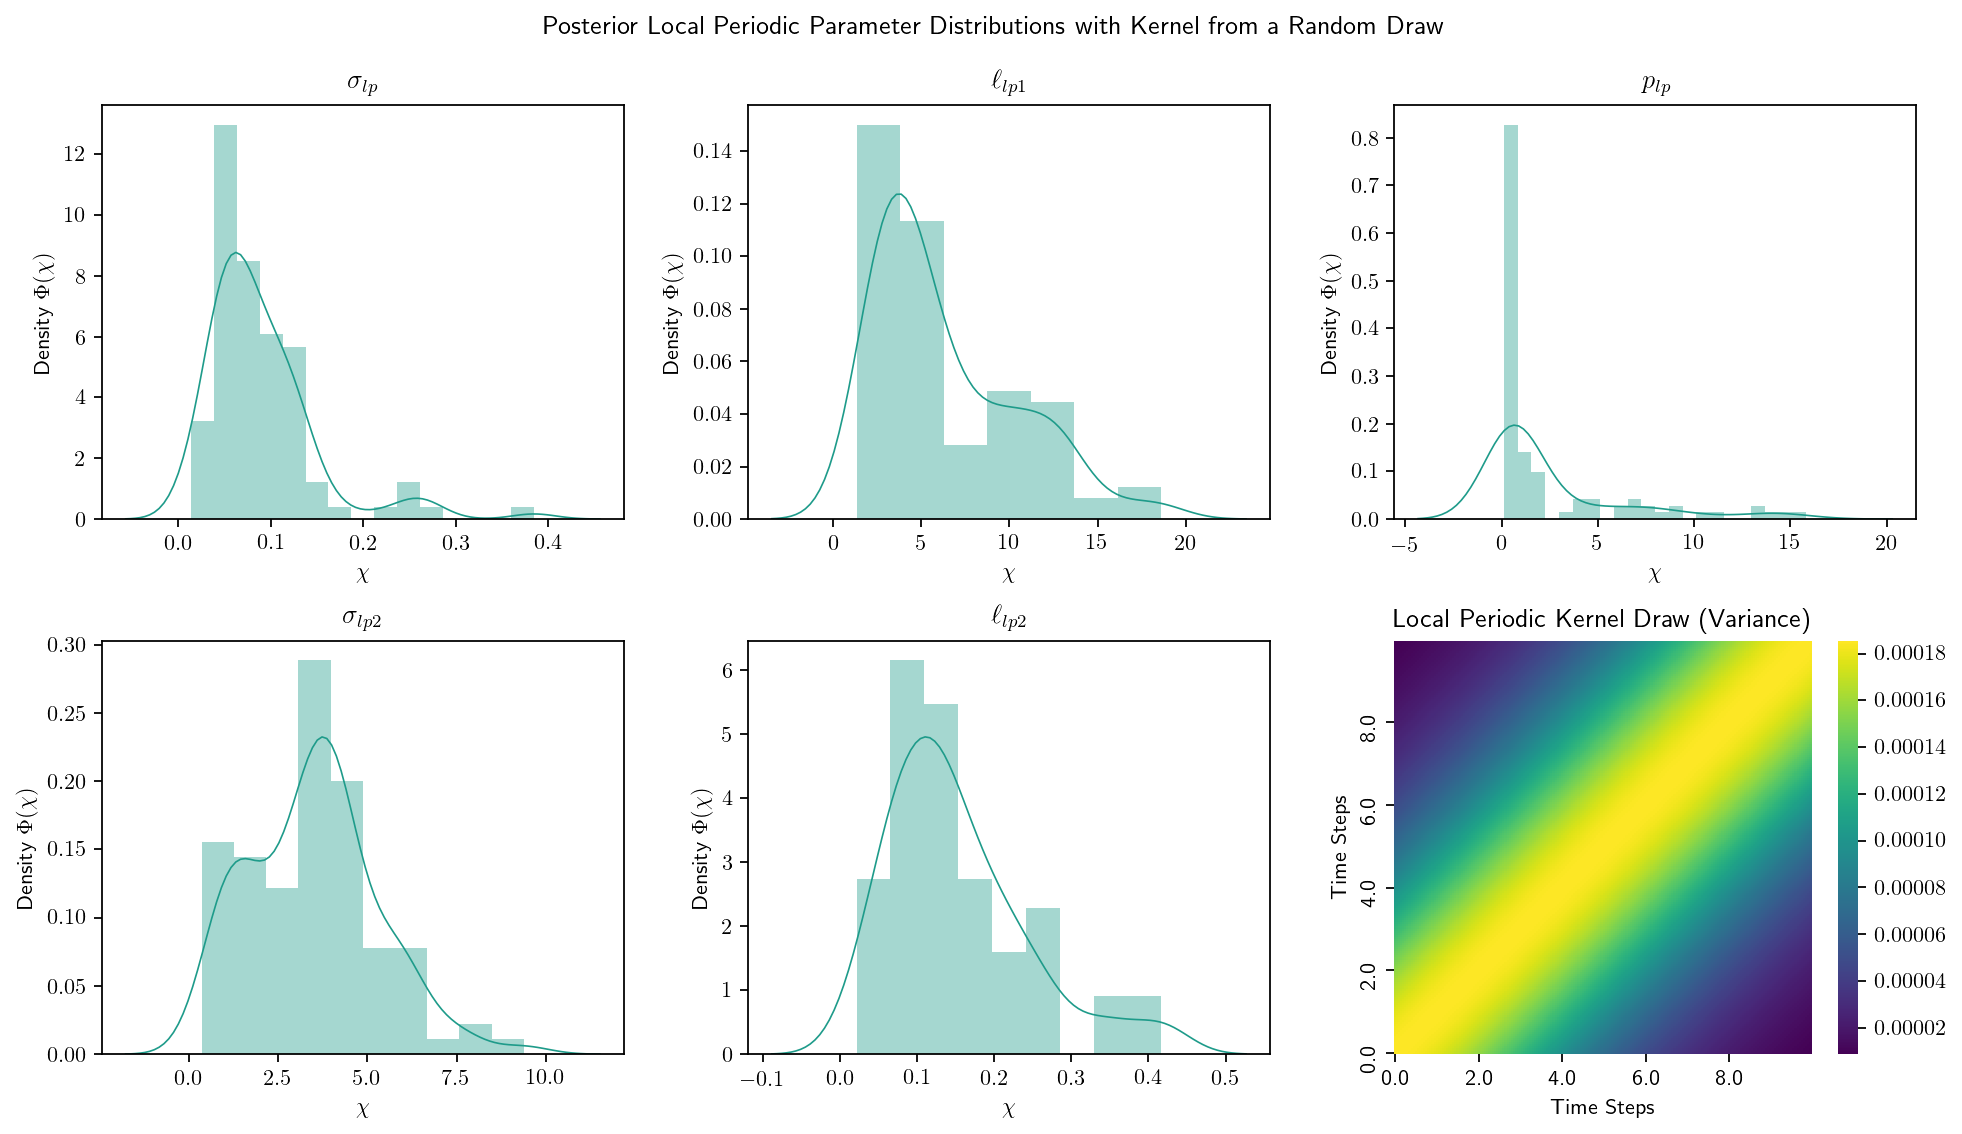
\includegraphics[width=1.2\textwidth,center]{img/gp/gp_kernel_posterior_local_periodic_zoomed.png}
	\caption{\textcolor{viridis5}{\textbf{Posterior Distributions}} for the local periodic kernel with example draw for the kernel.}
	\label{fig:gp_kernel_posterior_local_periodic}
\end{figure}

\begin{figure}[!hbt]
	\center
	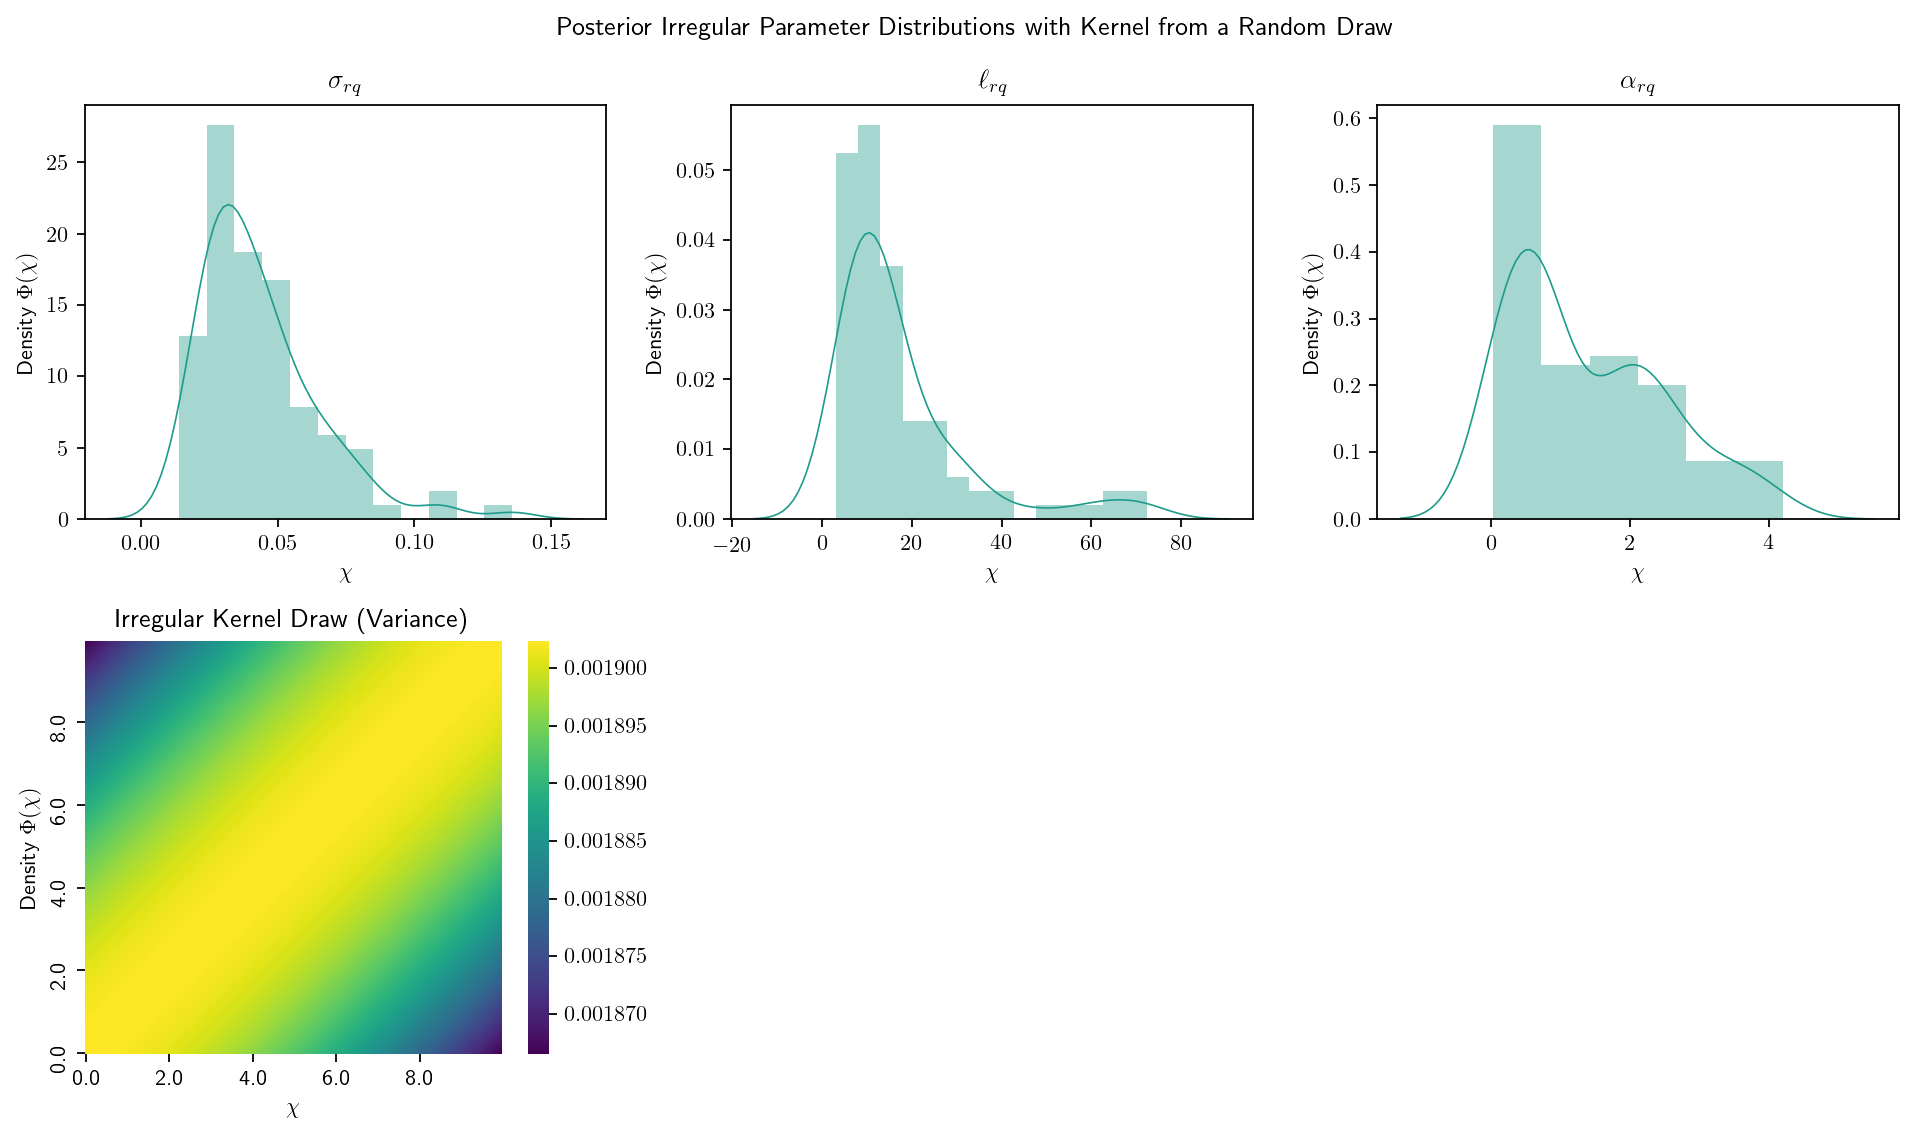
\includegraphics[width=1.2\textwidth,center]{img/gp/gp_kernel_posterior_irregular_zoomed.png}
	\caption{\textcolor{viridis5}{\textbf{Posterior Distributions}} for the irregular kernel with example draw for the kernel.}
	\label{fig:gp_kernel_posterior_irregular}
\end{figure}

\begin{figure}[!hbt]
	\center
	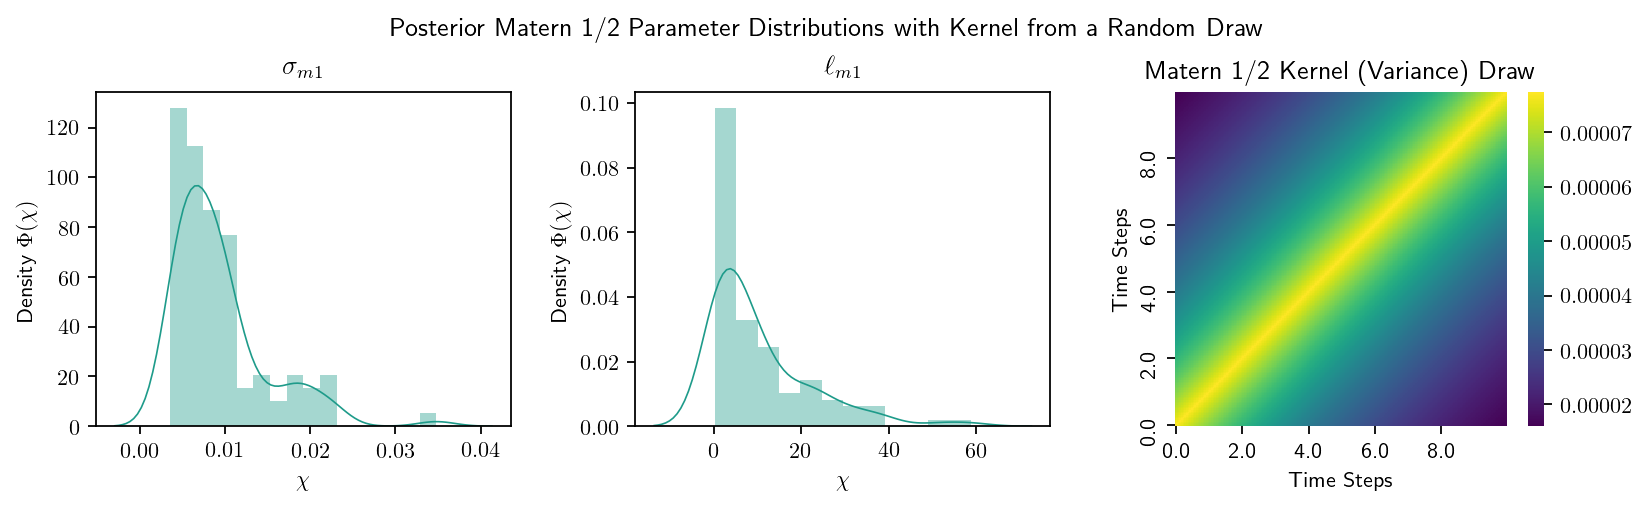
\includegraphics[width=1.2\textwidth,center]{img/gp/gp_kernel_posterior_matern1_zoomed.png}
	\caption{\textcolor{viridis5}{\textbf{Posterior Distributions}} for the Matérn 1/2 kernel with example draw for the kernel.}
	\label{fig:gp_kernel_posterior_matern1}
\end{figure}

\begin{figure}[!hbt]
	\center
	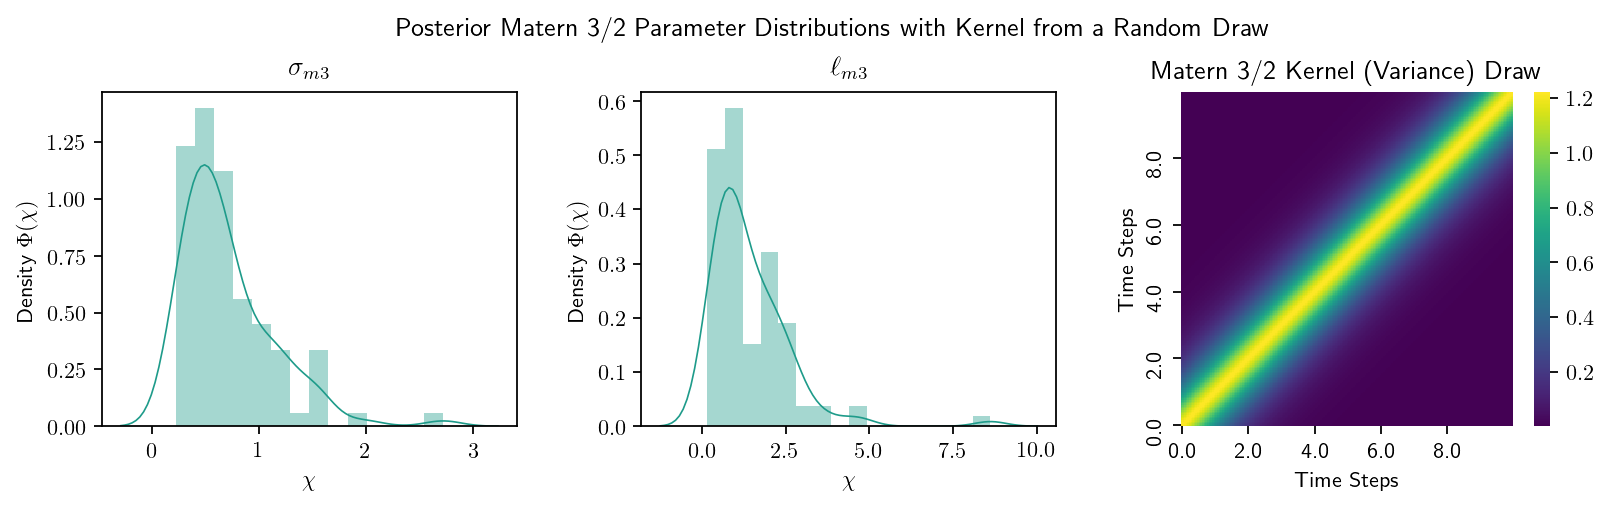
\includegraphics[width=1.2\textwidth,center]{img/gp/gp_kernel_posterior_matern3_zoomed.png}
	\caption{\textcolor{viridis5}{\textbf{Posterior Distributions}} for the Matérn 3/2 kernel with example draw for the kernel.}
	\label{fig:gp_kernel_posterior_matern3}
\end{figure}

\begin{figure}[!hbt]
	\center
	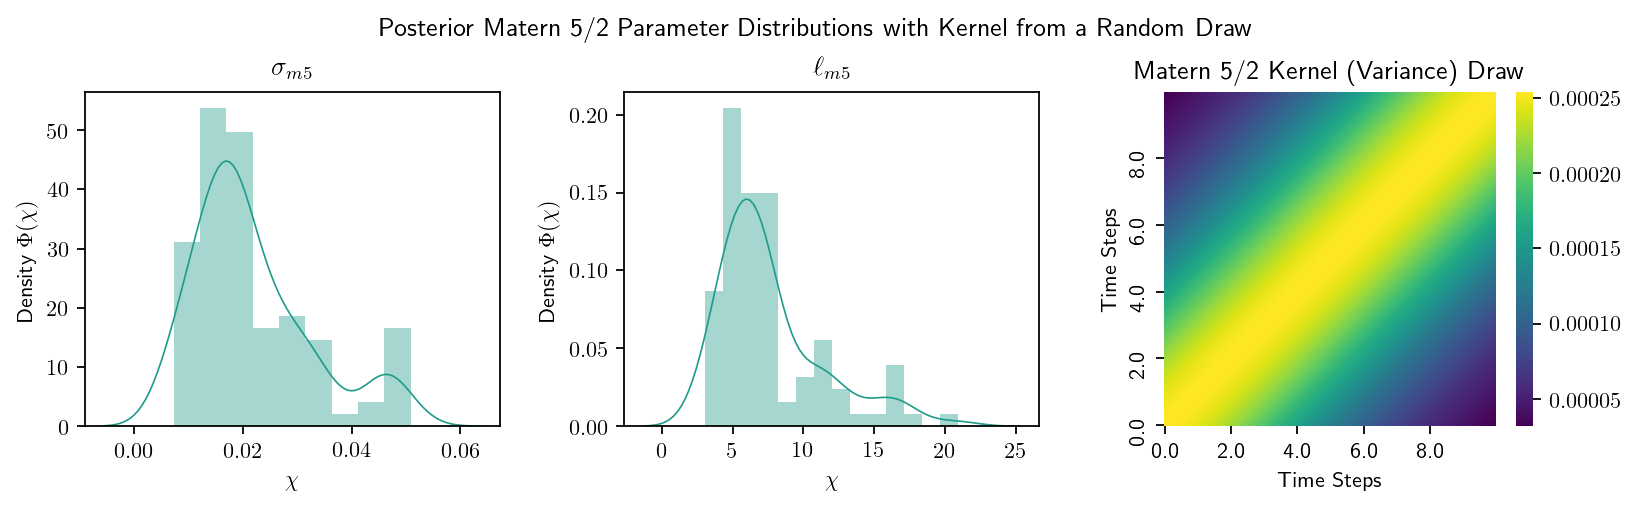
\includegraphics[width=1.2\textwidth,center]{img/gp/gp_kernel_posterior_matern5_zoomed.png}
	\caption{\textcolor{viridis5}{\textbf{Posterior Distributions}} for the Matérn 5/2 kernel with example draw for the kernel.}
	\label{fig:gp_kernel_posterior_matern5}
\end{figure}

%%% GDANSK DATA

%%% GDANSK DATA: NAIVE BAYES

\FloatBarrier
\subsection{Gdańsk: Naive Bayes}
\label{sec:original_gdansk_naive_bayes_classification}

\subsubsection{Error Distributions Classification}

\begin{figure}[!hbt]
	\makebox[\linewidth][c]{
		\centering
		\subfigure[Complete]{
			\label{fig:original_gdansk_naive_bayes_classification_complete_error_distribution}
			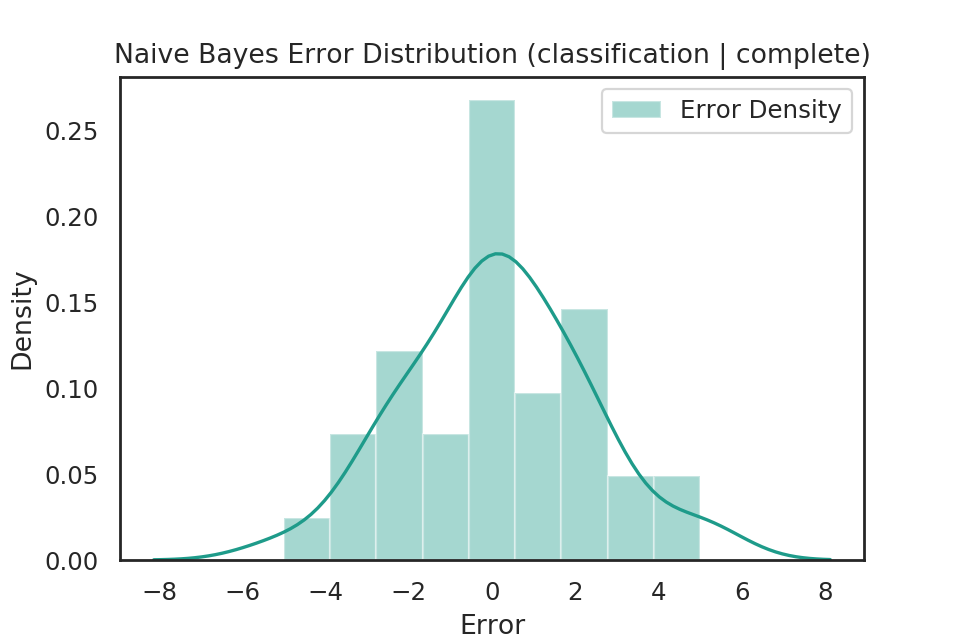
\includegraphics[width=0.6\textwidth]{img/learning/original_gdansk_naive_bayes_classification_complete_error_distribution}}
		\subfigure[Constant]{
			\label{fig:original_gdansk_naive_bayes_classification_constant_error_distribution}
			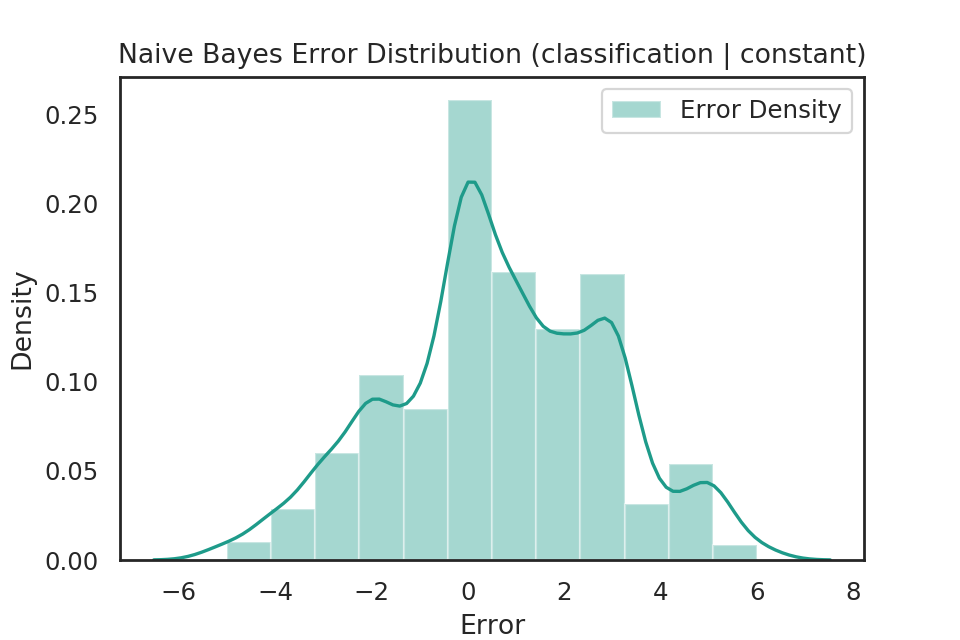
\includegraphics[width=0.6\textwidth]{img/learning/original_gdansk_naive_bayes_classification_constant_error_distribution}}
	}
	\caption{\textcolor{viridis5}{\textbf{Error distributions}} for Naive Bayes performing classification.}
\end{figure}

\subsubsection{Classification Metrics (Complete)}

\lstinputlisting{results/original_gdansk_naive_bayes_classification_complete_metrics.txt}

\subsubsection{Classification Metrics (Constant)}

\lstinputlisting{results/original_gdansk_naive_bayes_classification_constant_metrics.txt}


%%% GDANSK DATA: SVM

\FloatBarrier
\subsection{Gdańsk: Support Vector Machine}

\subsubsection{Error Distribution Classification}

\begin{figure}[!hbt]
	\makebox[\linewidth][c]{
		\centering
		\subfigure[Complete]{
			\label{fig:original_gdansk_svm_classification_complete_error_distribution}
			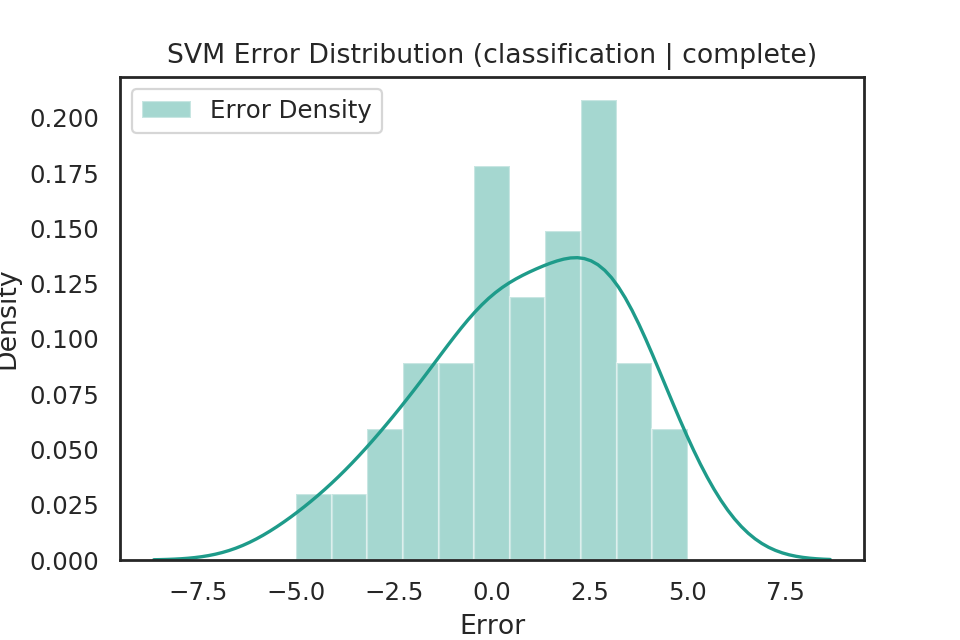
\includegraphics[width=0.6\textwidth]{img/learning/original_gdansk_svm_classification_complete_error_distribution}}
		\subfigure[Constant]{
			\label{fig:original_gdansk_svm_classification_constant_error_distribution}
			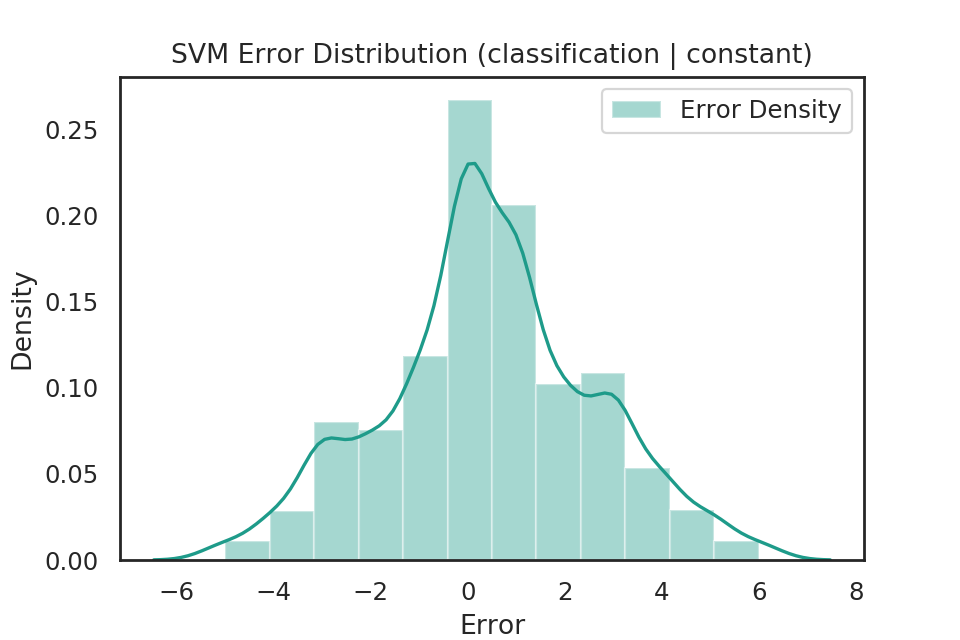
\includegraphics[width=0.6\textwidth]{img/learning/original_gdansk_svm_classification_constant_error_distribution}}
	}
	\caption{\textcolor{viridis5}{\textbf{Error distributions}} for SVM performing classification.}
\end{figure}

\FloatBarrier
\subsubsection{Classification Metrics (Complete)}

\lstinputlisting{results/original_gdansk_svm_classification_complete_metrics.txt}

\subsubsection{Classification Metrics (Constant)}

\lstinputlisting{results/original_gdansk_svm_classification_constant_metrics.txt}

\subsubsection{Error Distribution Regression}

\begin{figure}[!hbt]
	\makebox[\linewidth][c]{
		\centering
		\subfigure[Biased]{
			\label{fig:original_gdansk_svm_regression_complete_error_distribution}
			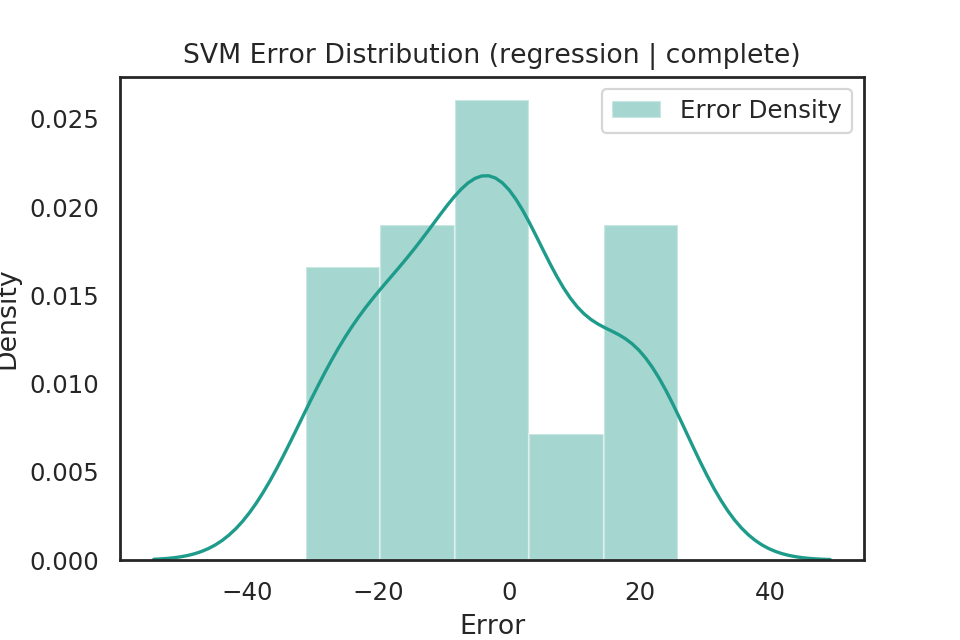
\includegraphics[width=0.6\textwidth]{img/learning/original_gdansk_svm_regression_complete_error_distribution.png}}
		\subfigure[Unbiased]{
			\label{fig:original_gdansk_svm_regression_complete_error_distribution_unbiased}
			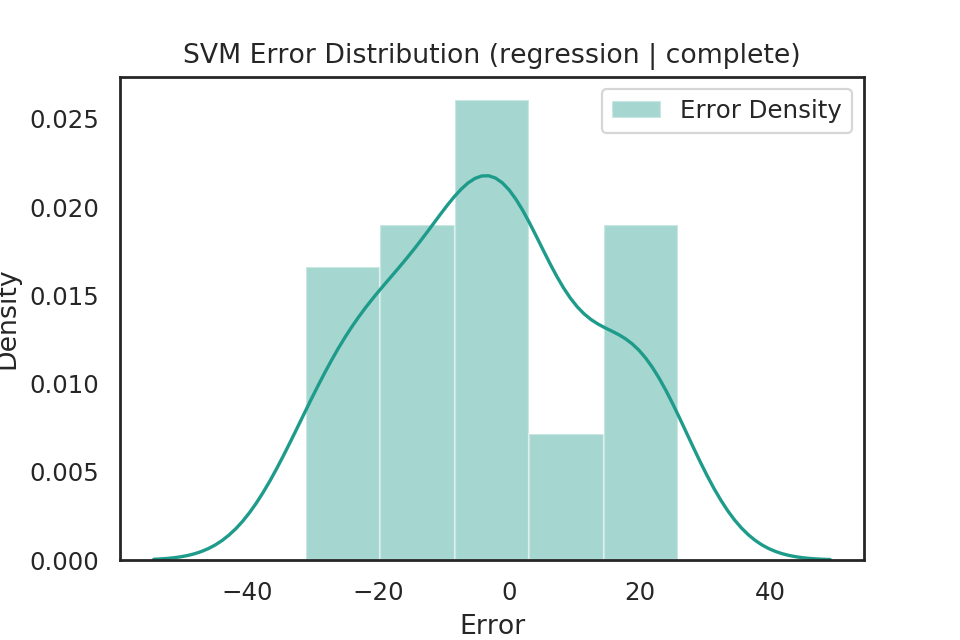
\includegraphics[width=0.6\textwidth]{img/learning/original_gdansk_svm_regression_complete_error_distribution.png}}
	}
	\caption{\textcolor{viridis5}{\textbf{Error distributions}} for SVM performing complete regression.}
\end{figure}

\begin{figure}[!hbt]
	\makebox[\linewidth][c]{
		\centering
		\subfigure[Biased]{
			\label{fig:original_gdansk_svm_regression_constant_error_distribution}
			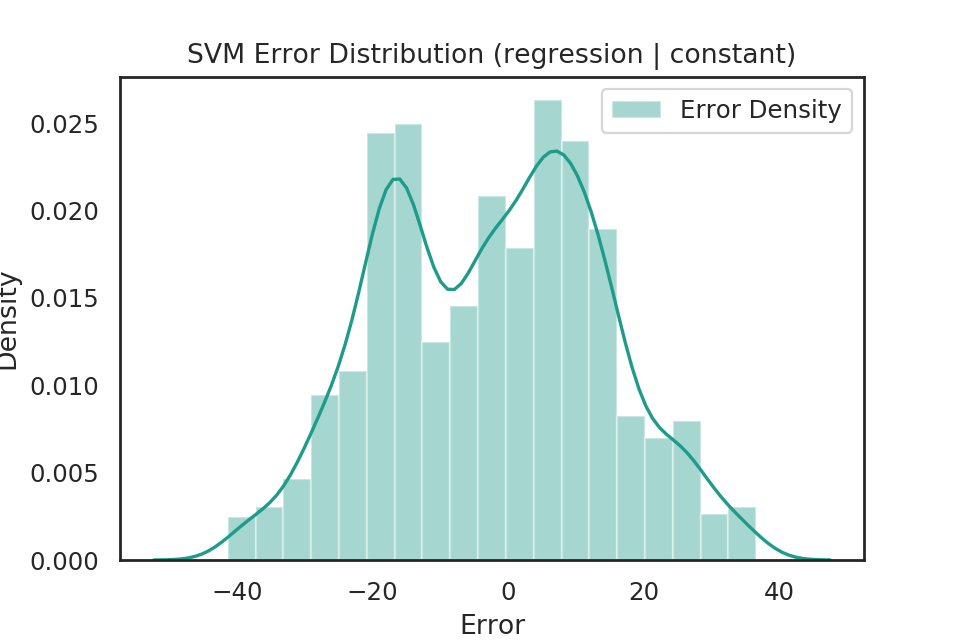
\includegraphics[width=0.6\textwidth]{img/learning/original_gdansk_svm_regression_constant_error_distribution.png}}
		\subfigure[Unbiased]{
			\label{fig:original_gdansk_svm_regression_constant_error_distribution_unbiased}
			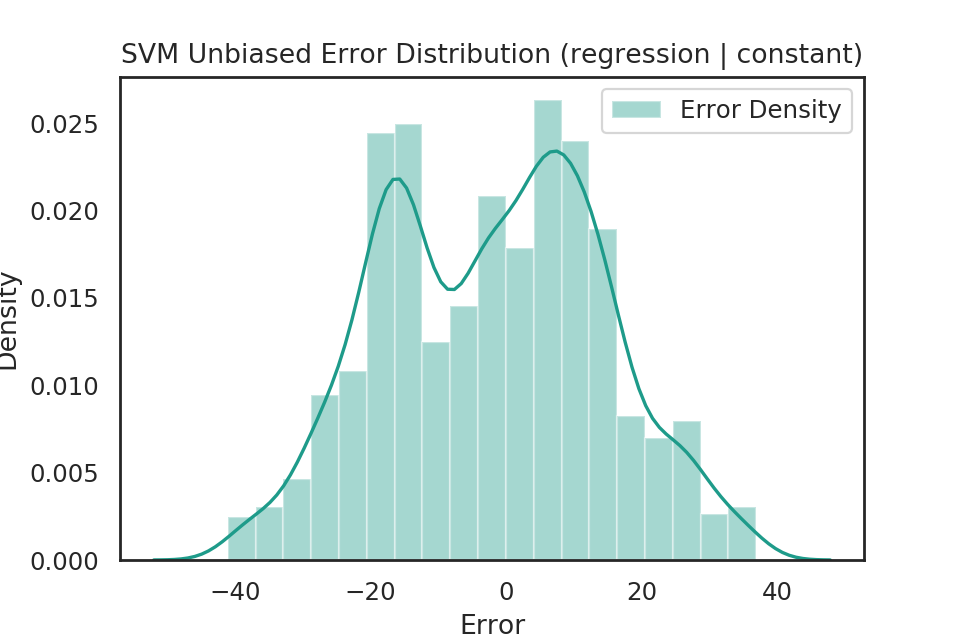
\includegraphics[width=0.6\textwidth]{img/learning/original_gdansk_svm_regression_constant_error_distribution_unbiased.png}}
	}
	\caption{\textcolor{viridis5}{\textbf{Error distributions}} for SVM performing constant regression.}
\end{figure}

\FloatBarrier
\subsubsection{Metrics (Complete)}

\lstinputlisting{results/original_gdansk_svm_regression_complete_metrics.txt}

\subsubsection{Metrics (Constant)}

\lstinputlisting{results/original_gdansk_svm_regression_constant_metrics.txt}


%%% GDANSK DATA: RANDOM FOREST

\FloatBarrier
\subsection{Gdańsk: Random Forest}

\subsubsection{Error Distribution Classification}

\begin{figure}[!hbt]
	\makebox[\linewidth][c]{
		\centering
		\subfigure[Complete]{
			\label{fig:original_gdansk_random_forest_classification_complete_error_distribution}
			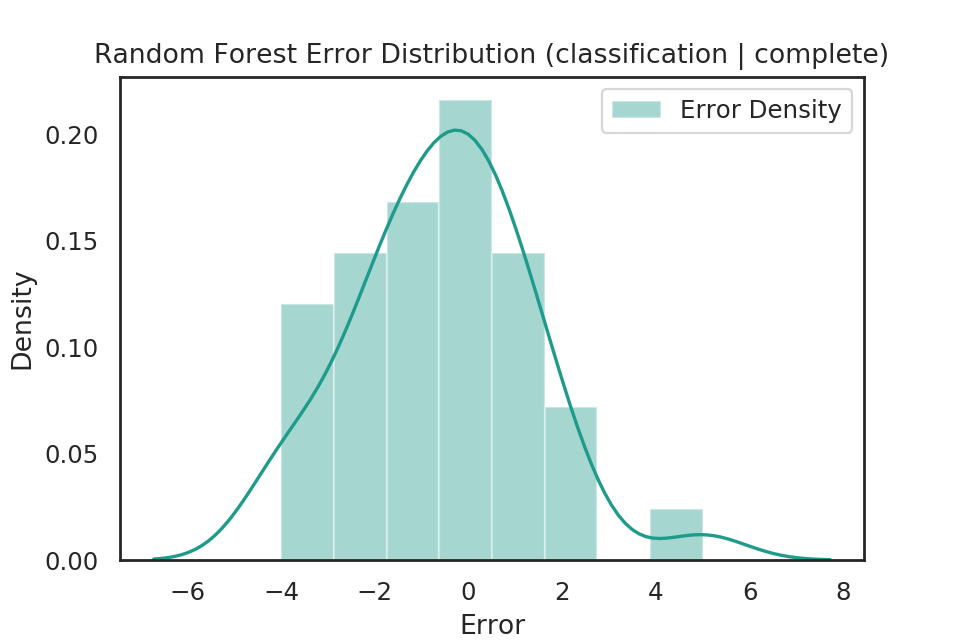
\includegraphics[width=0.6\textwidth]{img/learning/original_gdansk_random_forest_classification_complete_error_distribution.png}}
		\subfigure[Constant]{
			\label{fig:original_gdansk_random_forest_classification_constant_error_distribution}
			\includegraphics[width=0.6\textwidth]{img/learning/original_gdansk_random_forest_classification_constant_error_distribution}}
	}
	\caption{\textcolor{viridis5}{\textbf{Error distributions}} for Random Forest performing classification.}
\end{figure}

\FloatBarrier
\subsubsection{Classification Metrics (Complete)}

\lstinputlisting{results/original_gdansk_random_forest_classification_complete_metrics.txt}

\subsubsection{Classification Metrics (Constant)}

\lstinputlisting{results/original_gdansk_random_forest_classification_constant_metrics.txt}

\subsubsection{Error Distribution Regression}

\begin{figure}[!hbt]
	\makebox[\linewidth][c]{
		\centering
		\subfigure[Biased]{
			\label{fig:original_gdansk_random_forest_regression_complete_error_distribution}
			\includegraphics[width=0.6\textwidth]{img/learning/original_gdansk_random_forest_regression_complete_error_distribution.png}}
		\subfigure[Unbiased]{			\label{fig:original_gdansk_random_forest_regression_complete_error_distribution_unbiased}
			\includegraphics[width=0.6\textwidth]{img/learning/original_gdansk_random_forest_regression_complete_error_distribution_unbiased.png}}
	}
	\caption{\textcolor{viridis5}{\textbf{Error distributions}} for Random Forest performing complete regression.}
\end{figure}

\begin{figure}[!hbt]
	\makebox[\linewidth][c]{
		\centering
		\subfigure[Biased]{
			\label{fig:original_gdansk_random_forest_regression_constant_error_distribution}
			\includegraphics[width=0.6\textwidth]{img/learning/original_gdansk_random_forest_regression_constant_error_distribution.png}}
		\subfigure[Unbiased]{			\label{fig:original_gdansk_random_forest_regression_constant_error_distribution_unbiased}
			\includegraphics[width=0.6\textwidth]{img/learning/original_gdansk_random_forest_regression_constant_error_distribution_unbiased.png}}
	}
	\caption{\textcolor{viridis5}{\textbf{Error distributions}} for Random Forest performing constant regression.}
\end{figure}

\FloatBarrier
\subsubsection{Regression Metrics (Complete)}

\lstinputlisting{results/original_gdansk_random_forest_regression_complete_metrics.txt}

\subsubsection{Regression Metrics (Constant)}

\lstinputlisting{results/original_gdansk_random_forest_regression_constant_metrics.txt}


%%% GDANSK DATA: XGBOOST

\FloatBarrier
\subsection{Gdańsk: XGBoost}

\subsubsection{Error Distribution Classification}

\begin{figure}[!hbt]
	\makebox[\linewidth][c]{
		\centering
		\subfigure[Complete]{
			\label{fig:original_gdansk_xgboost_classification_complete_error_distribution}
			\includegraphics[width=0.6\textwidth]{img/learning/original_gdansk_xgboost_classification_complete_error_distribution.png}}
		\subfigure[Constant]{
			\label{fig:original_gdansk_xgboost_classification_constant_error_distribution}
			\includegraphics[width=0.6\textwidth]{img/learning/original_gdansk_xgboost_classification_constant_error_distribution.png}}
	}
	\caption{\textcolor{viridis5}{\textbf{Error distributions}} for XGBoost performing classification.}
\end{figure}

\FloatBarrier
\subsubsection{Classification Metrics (Complete)}

\lstinputlisting{results/original_gdansk_xgboost_classification_complete_metrics.txt}

\subsubsection{Classification Metrics (Constant)}

\lstinputlisting{results/original_gdansk_xgboost_classification_constant_metrics.txt}

\subsubsection{Error Distribution Regression}

\begin{figure}[!hbt]
	\makebox[\linewidth][c]{
		\centering
		\subfigure[Biased]{
			\label{fig:original_gdansk_xgboost_regression_complete_error_distribution}
			\includegraphics[width=0.6\textwidth]{img/learning/original_gdansk_xgboost_regression_complete_error_distribution.png}}
		\subfigure[Unbiased]{
			\label{fig:original_gdansk_xgboost_regression_complete_error_distribution_unbiased}
			\includegraphics[width=0.6\textwidth]{img/learning/original_gdansk_xgboost_regression_complete_error_distribution_unbiased.png}}
	}
	\caption{\textcolor{viridis5}{\textbf{Error distributions}} for XGBoost performing complete regression.}
\end{figure}

\begin{figure}[!hbt]
	\makebox[\linewidth][c]{
		\centering
		\subfigure[Biased]{
			\label{fig:original_gdansk_xgboost_regression_constant_error_distribution}
			\includegraphics[width=0.6\textwidth]{img/learning/original_gdansk_xgboost_regression_constant_error_distribution.png}}
		\subfigure[Unbiased]{
			\label{fig:original_gdansk_xgboost_regression_constant_error_distribution_unbiased}
			\includegraphics[width=0.6\textwidth]{img/learning/original_gdansk_xgboost_regression_constant_error_distribution_unbiased.png}}
	}
	\caption{\textcolor{viridis5}{\textbf{Error distributions}} for XGBoost performing constant regression.}
\end{figure}

\FloatBarrier
\subsubsection{Regression Metrics (Complete)}

\lstinputlisting{results/original_gdansk_xgboost_regression_complete_metrics.txt}

\subsubsection{Regression Metrics (Constant)}

\lstinputlisting{results/original_gdansk_xgboost_regression_constant_metrics.txt}


%%% GDANSK DATA: DEEPSLEEP (COMPLETE / CLASSIFICATION)

\FloatBarrier
\subsection{Gdańsk: DeepSleep}
\label{sec:gdansk_deepsleep}

\FloatBarrier
\subsubsection{Complete Classification (standard)}

\begin{figure}[!hbt]
    \makebox[\linewidth][c]{
	\centering
	\subfigure[Loss]{\label{fig:original_gdansk_sleepnet_classification_complete_none_unweighted_loss}\includegraphics[width=0.6\textwidth]{img/learning/original_gdansk_sleepnet_classification_complete_none_unweighted_loss.png}}
	\subfigure[Accuracy]{\label{fig:original_gdansk_sleepnet_classification_complete_none_unweighted_accuracy}\includegraphics[width=0.6\textwidth]{img/learning/original_gdansk_sleepnet_classification_complete_none_unweighted_accuracy.png}}
	}
	\caption{\textcolor{viridis9}{\textbf{Training}} and \textcolor{viridis0}{\textbf{validation}} loss and accuracy for DeepSleep performing standard complete classification.}
\end{figure}

\begin{figure}[hbt]
	\centering
	\includegraphics[width=0.6\textwidth,center]{img/learning/original_gdansk_sleepnet_classification_complete_none_unweighted_error_distribution.png}
	\caption{\textcolor{viridis5}{\textbf{Error distribution}} for DeepSleep performing standard complete classification.}
	\label{fig:original_gdansk_sleepnet_classification_complete_none_unweighted_error_distribution}
\end{figure}

\FloatBarrier

\lstinputlisting{results/original_gdansk_sleepnet_classification_complete_none_unweighted_metrics.txt}

\FloatBarrier
\subsubsection{Complete Classification (weighted)}

\begin{figure}[!hbt]
    \makebox[\linewidth][c]{
	\centering
	\subfigure[Loss]{\label{fig:original_gdansk_sleepnet_classification_complete_none_weighted_loss}\includegraphics[width=0.6\textwidth]{img/learning/original_gdansk_sleepnet_classification_complete_none_weighted_loss.png}}
	\subfigure[Accuracy]{\label{fig:original_gdansk_sleepnet_classification_complete_none_weighted_accuracy}\includegraphics[width=0.6\textwidth]{img/learning/original_gdansk_sleepnet_classification_complete_none_weighted_accuracy.png}}
	}
	\caption{\textcolor{viridis9}{\textbf{Training}} and \textcolor{viridis0}{\textbf{validation}} loss and accuracy for DeepSleep performing weighted complete classification.}
\end{figure}

\begin{figure}[hbt]
	\centering
	\includegraphics[width=0.6\textwidth,center]{img/learning/original_gdansk_sleepnet_classification_complete_none_weighted_error_distribution.png}
	\caption{\textcolor{viridis5}{\textbf{Error distribution}} for DeepSleep performing weighted complete classification.}
	\label{fig:original_gdansk_sleepnet_classification_complete_none_weighted_error_distribution}
\end{figure}

\FloatBarrier
\lstinputlisting{results/original_gdansk_sleepnet_classification_constant_none_weighted_metrics.txt}

\FloatBarrier
\subsubsection{Complete Classification (oversampled)}

\begin{figure}[!hbt]
    \makebox[\linewidth][c]{
	\centering
	\subfigure[Loss]{\label{fig:original_gdansk_sleepnet_classification_complete_oversample_unweighted_loss}\includegraphics[width=0.6\textwidth]{img/learning/original_gdansk_sleepnet_classification_complete_oversample_unweighted_loss.png}}
	\subfigure[Accuracy]{\label{fig:original_gdansk_sleepnet_classification_complete_oversample_unweighted_accuracy}\includegraphics[width=0.6\textwidth]{img/learning/original_gdansk_sleepnet_classification_complete_oversample_unweighted_accuracy.png}}
	}
	\caption{\textcolor{viridis9}{\textbf{Training}} and \textcolor{viridis0}{\textbf{validation}} loss and accuracy for DeepSleep performing oversampled complete classification.}
\end{figure}

\begin{figure}[hbt]
	\centering
	\includegraphics[width=0.6\textwidth]{img/learning/original_gdansk_sleepnet_classification_complete_oversample_unweighted_error_distribution.png}
	\caption{\textcolor{viridis5}{\textbf{Error distribution}} for DeepSleep performing oversample complete classification.}
	\label{fig:original_gdansk_sleepnet_classification_complete_oversample_unweighted_error_distribution}
\end{figure}

\FloatBarrier
\lstinputlisting{results/original_gdansk_sleepnet_classification_complete_oversample_unweighted_metrics.txt}


%%% GDANSK DATA: DEEPSLEEP (CONSTANT / CLASSIFICATION)

\FloatBarrier
\subsubsection{Constant Classification (standard)}

\begin{figure}[!hbt]
    \makebox[\linewidth][c]{
	\centering
	\subfigure[Loss]{\label{fig:original_gdansk_sleepnet_classification_constant_none_unweighted_loss}\includegraphics[width=0.6\textwidth]{img/learning/original_gdansk_sleepnet_classification_constant_none_unweighted_loss.png}}
	\subfigure[Accuracy]{\label{fig:original_gdansk_sleepnet_classification_constant_none_unweighted_accuracy}\includegraphics[width=0.6\textwidth]{img/learning/original_gdansk_sleepnet_classification_constant_none_unweighted_accuracy.png}}
	}
	\caption{\textcolor{viridis9}{\textbf{Training}} and \textcolor{viridis0}{\textbf{validation}} loss and accuracy for DeepSleep performing standard constant classification.}
\end{figure}

\begin{figure}[hbt]
	\centering
	\includegraphics[width=0.6\textwidth]{img/learning/original_gdansk_sleepnet_classification_constant_none_unweighted_error_distribution.png}
	\caption{\textcolor{viridis5}{\textbf{Error distribution}} for DeepSleep performing standard constant classification.}
	\label{fig:original_gdansk_sleepnet_classification_constant_none_unweighted_error_distribution}
\end{figure}

\FloatBarrier

\lstinputlisting{results/original_gdansk_sleepnet_classification_constant_none_unweighted_metrics.txt}

\FloatBarrier
\subsubsection{Constant Classification (weighted)}

\begin{figure}[!hbt]
    \makebox[\linewidth][c]{
	\centering
	\subfigure[Loss]{\label{fig:original_gdansk_sleepnet_classification_constant_none_weighted_loss}\includegraphics[width=0.6\textwidth]{img/learning/original_gdansk_sleepnet_classification_constant_none_weighted_loss.png}}
	\subfigure[Accuracy]{\label{fig:original_gdansk_sleepnet_classification_constant_none_weighted_accuracy}\includegraphics[width=0.6\textwidth]{img/learning/original_gdansk_sleepnet_classification_constant_none_weighted_accuracy.png}}
	}
	\caption{\textcolor{viridis9}{\textbf{Training}} and \textcolor{viridis0}{\textbf{validation}} loss and accuracy for DeepSleep performing weighted constant classification.}
\end{figure}

\begin{figure}[hbt]
	\centering
	\includegraphics[width=0.6\textwidth]{img/learning/original_gdansk_sleepnet_classification_constant_none_weighted_error_distribution.png}
	\caption{\textcolor{viridis5}{\textbf{Error distributions}} for DeepSleep performing weighted constant classification.}
	\label{fig:original_gdansk_sleepnet_classification_constant_none_weighted_error_distribution}
\end{figure}

\FloatBarrier

\lstinputlisting{results/original_gdansk_sleepnet_classification_constant_none_weighted_metrics.txt}

\FloatBarrier
\subsubsection{Constant Classification (oversampled)}

\begin{figure}[!hbt]
    \makebox[\linewidth][c]{
	\centering
	\subfigure[Loss]{\label{fig:original_gdansk_sleepnet_classification_constant_oversample_unweighted_loss}\includegraphics[width=0.6\textwidth]{img/learning/original_gdansk_sleepnet_classification_constant_oversample_unweighted_loss.png}}
	\subfigure[Accuracy]{\label{fig:original_gdansk_sleepnet_classification_constant_oversample_unweighted_accuracy}\includegraphics[width=0.6\textwidth]{img/learning/original_gdansk_sleepnet_classification_constant_oversample_unweighted_accuracy.png}}
	}
	\caption{\textcolor{viridis9}{\textbf{Training}} and \textcolor{viridis0}{\textbf{validation}} loss and accuracy for DeepSleep performing oversampled constant classification.}
\end{figure}

\begin{figure}[hbt]
	\centering
	\includegraphics[width=0.6\textwidth]{img/learning/original_gdansk_sleepnet_classification_constant_oversample_unweighted_error_distribution.png}
	\caption{\textcolor{viridis5}{\textbf{Error distribution}} for DeepSleep performing oversample constant classification.}
	\label{fig:original_gdansk_sleepnet_classification_constant_oversample_unweighted_error_distribution}
\end{figure}

\FloatBarrier
\lstinputlisting{results/original_gdansk_sleepnet_classification_constant_oversample_unweighted_metrics.txt}


%%% GDANSK DATA: DEEPSLEEP (COMPLETE / REGRESSION)

\FloatBarrier
\subsubsection{Complete Regression (standard)}

\begin{figure}[!hbt]
    \makebox[\linewidth][c]{
	\centering
	\subfigure[Loss]{\label{fig:original_gdansk_sleepnet_regression_complete_none_loss}\includegraphics[width=0.6\textwidth]{img/learning/original_gdansk_sleepnet_regression_complete_none_loss.png}}
	\subfigure[Accuracy]{\label{fig:original_gdansk_sleepnet_regression_complete_none_accuracy}\includegraphics[width=0.6\textwidth]{img/learning/original_gdansk_sleepnet_regression_complete_none_accuracy.png}}
	}
	\caption{\textcolor{viridis9}{\textbf{Training}} and \textcolor{viridis0}{\textbf{validation}} loss and accuracy for DeepSleep performing standard complete regression.}
\end{figure}

\begin{figure}[!hbt]
    \makebox[\linewidth][c]{
	\centering
	\subfigure[Biased]{\label{fig:original_gdansk_sleepnet_regression_complete_none_error_distribution}\includegraphics[width=0.6\textwidth]{img/learning/original_gdansk_sleepnet_regression_complete_none_error_distribution.png}}
	\subfigure[Unbiased]{\label{fig:original_gdansk_sleepnet_regression_complete_none_error_distribution_unbiased}\includegraphics[width=0.6\textwidth]{img/learning/original_gdansk_sleepnet_regression_complete_none_error_distribution_unbiased.png}}
	}
	\caption{\textcolor{viridis5}{\textbf{Error distributions}} for DeepSleep performing standard complete regression.}
\end{figure}

\FloatBarrier

\lstinputlisting{results/original_gdansk_sleepnet_regression_complete_none_metrics.txt}

\FloatBarrier
\subsubsection{Complete Regression (oversampled)}

\begin{figure}[!hbt]
    \makebox[\linewidth][c]{
	\centering
	\subfigure[Loss]
	{\label{fig:original_gdansk_sleepnet_regression_complete_oversample_loss}\includegraphics[width=0.6\textwidth]{img/learning/original_gdansk_sleepnet_regression_complete_oversample_loss.png}}
	\subfigure[Accuracy]{\label{fig:original_gdansk_sleepnet_regression_complete_oversample_accuracy}\includegraphics[width=0.6\textwidth]{img/learning/original_gdansk_sleepnet_regression_complete_oversample_accuracy.png}}
	}
	\caption{\textcolor{viridis9}{\textbf{Training}} and \textcolor{viridis0}{\textbf{validation}} loss and accuracy for DeepSleep performing oversampled complete regression.}
\end{figure}

\begin{figure}[!hbt]
    \makebox[\linewidth][c]{
	\centering
	\subfigure[Biased]{\label{fig:original_gdansk_sleepnet_regression_complete_oversample_error_distribution}
	\includegraphics[width=0.6\textwidth]{img/learning/original_gdansk_sleepnet_regression_complete_oversample_error_distribution.png}
	}
	\subfigure[Unbiased]{\label{fig:original_gdansk_sleepnet_regression_complete_oversample_error_distribution_unbiased}
	\includegraphics[width=0.6\textwidth]{img/learning/original_gdansk_sleepnet_regression_complete_oversample_error_distribution_unbiased.png}
	}
	}
	\caption{\textcolor{viridis5}{\textbf{Error distributions}} for DeepSleep performing oversampled complete regression.}
\end{figure}

\FloatBarrier
\lstinputlisting{results/original_gdansk_sleepnet_regression_complete_none_metrics.txt}


%%% GDANSK DATA: DEEPSLEEP (CONSTANT / REGRESSION)

\FloatBarrier
\subsubsection{Constant Regression (standard)}

\begin{figure}[!hbt]
    \makebox[\linewidth][c]{
	\centering
	\subfigure[Loss]{\label{fig:original_gdansk_sleepnet_regression_constant_none_loss}\includegraphics[width=0.6\textwidth]{img/learning/original_gdansk_sleepnet_regression_constant_none_loss.png}}
	\subfigure[Accuracy]{\label{fig:original_gdansk_sleepnet_regression_constant_none_accuracy}\includegraphics[width=0.6\textwidth]{img/learning/original_gdansk_sleepnet_regression_constant_none_accuracy.png}}
	}
	\caption{\textcolor{viridis9}{\textbf{Training}} and \textcolor{viridis0}{\textbf{validation}} loss and accuracy for DeepSleep performing standard constant regression.}
\end{figure}

\begin{figure}[!hbt]
    \makebox[\linewidth][c]{
	\centering
	\subfigure[Biased]{\label{fig:original_gdansk_sleepnet_regression_constant_none_error_distribution}\includegraphics[width=0.6\textwidth]{img/learning/original_gdansk_sleepnet_regression_constant_none_error_distribution.png}}
	\subfigure[Unbiased]{\label{fig:original_gdansk_sleepnet_regression_constant_none_error_distribution_unbiased}\includegraphics[width=0.6\textwidth]{img/learning/original_gdansk_sleepnet_regression_constant_none_error_distribution_unbiased.png}}
	}
	\caption{\textcolor{viridis5}{\textbf{Error distributions}} for DeepSleep performing standard constant regression.}
\end{figure}

\FloatBarrier

\lstinputlisting{results/original_gdansk_sleepnet_regression_constant_none_metrics.txt}


\FloatBarrier
\subsubsection{Constant Regression (oversampled)}

\begin{figure}[!hbt]
    \makebox[\linewidth][c]{
	\centering
	\subfigure[Loss]{\label{fig:original_gdansk_sleepnet_regression_constant_oversample_loss}\includegraphics[width=0.6\textwidth]{img/learning/original_gdansk_sleepnet_regression_constant_oversample_loss.png}}
	\subfigure[Accuracy]{\label{fig:original_gdansk_sleepnet_regression_constant_oversample_accuracy}\includegraphics[width=0.6\textwidth]{img/learning/original_gdansk_sleepnet_regression_constant_oversample_accuracy.png}}
	}
	\caption{\textcolor{viridis9}{\textbf{Training}} and \textcolor{viridis0}{\textbf{validation}} loss and accuracy for DeepSleep performing oversampled constant regression.}
\end{figure}

\begin{figure}[!hbt]
    \makebox[\linewidth][c]{
	\centering
	\subfigure[Biased]{\label{fig:original_gdansk_sleepnet_regression_constant_oversample_error_distribution}\includegraphics[width=0.6\textwidth]{img/learning/original_gdansk_sleepnet_regression_constant_oversample_error_distribution.png}}
	\subfigure[Unbiased]{\label{fig:original_gdansk_sleepnet_regression_constant_oversample_error_distribution_unbiased}\includegraphics[width=0.6\textwidth]{img/learning/original_gdansk_sleepnet_regression_constant_oversample_error_distribution_unbiased.png}}
	}
	\caption{\textcolor{viridis5}{\textbf{Error distributions}} for DeepSleep performing oversampled constant regression.}
\end{figure}

\FloatBarrier

\lstinputlisting{results/original_gdansk_sleepnet_regression_constant_none_metrics.txt}


%%% PHYSIONET DATA

%%% PHYSIONET DATA: NAIVE BAYES

\FloatBarrier
\subsection{Physionet: Naive Bayes}
\label{sec:original_physionet_naive_bayes_classification}

\subsubsection{Error Distributions Classification}

\begin{figure}[!hbt]
	\makebox[\linewidth][c]{
		\centering
		\subfigure[Complete]{
			\label{fig:original_physionet_naive_bayes_classification_complete_error_distribution}
			\includegraphics[width=0.6\textwidth]{img/learning/original_physionet_naive_bayes_classification_complete_error_distribution}}
		\subfigure[Constant]{
			\label{fig:original_physionet_naive_bayes_classification_constant_error_distribution}
			\includegraphics[width=0.6\textwidth]{img/learning/original_physionet_naive_bayes_classification_constant_error_distribution}}
	}
	\caption{\textcolor{viridis5}{\textbf{Error distributions}} for Naive Bayes performing classification.}
\end{figure}

\FloatBarrier
\subsubsection{Classification Metrics (Complete)}

\lstinputlisting{results/original_physionet_naive_bayes_classification_complete_metrics.txt}

\subsubsection{Classification Metrics (Constant)}

\lstinputlisting{results/original_physionet_naive_bayes_classification_constant_metrics.txt}

%%% PHYSIONET DATA: SVM

\FloatBarrier
\subsection{Physionet: Support Vector Machine}

\subsubsection{Error Distribution Classification}

\begin{figure}[!hbt]
	\makebox[\linewidth][c]{
		\centering
		\subfigure[Complete]{
			\label{fig:original_physionet_svm_classification_complete_error_distribution}
			\includegraphics[width=0.6\textwidth]{img/learning/original_physionet_svm_classification_complete_error_distribution}}
		\subfigure[Constant]{
			\label{fig:original_physionet_svm_classification_constant_error_distribution}
			\includegraphics[width=0.6\textwidth]{img/learning/original_physionet_svm_classification_constant_error_distribution}}
	}
	\caption{\textcolor{viridis5}{\textbf{Error distributions}} for SVM performing classification.}
\end{figure}

\FloatBarrier
\subsubsection{Classification Metrics (Complete)}

\lstinputlisting{results/original_physionet_svm_classification_complete_metrics.txt}

\subsubsection{Classification Metrics (Constant)}

\lstinputlisting{results/original_physionet_svm_classification_constant_metrics.txt}

\subsubsection{Error Distribution Regression}

\begin{figure}[!hbt]
	\makebox[\linewidth][c]{
		\centering
		\subfigure[Biased]{
			\label{fig:original_physionet_svm_regression_complete_error_distribution}
			\includegraphics[width=0.6\textwidth]{img/learning/original_physionet_svm_regression_complete_error_distribution.png}}
		\subfigure[Unbiased]{
			\label{fig:original_physionet_svm_regression_complete_error_distribution_unbiased}
			\includegraphics[width=0.6\textwidth]{img/learning/original_physionet_svm_regression_complete_error_distribution_unbiased.png}}
	}
	\caption{\textcolor{viridis5}{\textbf{Error distributions}} for SVM performing complete regression.}
\end{figure}

\begin{figure}[!hbt]
	\makebox[\linewidth][c]{
		\centering
		\subfigure[Biased]{
			\label{fig:original_physionet_svm_regression_constant_error_distribution}
			\includegraphics[width=0.6\textwidth]{img/learning/original_physionet_svm_regression_constant_error_distribution.png}}
		\subfigure[Unbiased]{
			\label{fig:original_physionet_svm_regression_constant_error_distribution_unbiased}
			\includegraphics[width=0.6\textwidth]{img/learning/original_physionet_svm_regression_constant_error_distribution_unbiased.png}}
	}
	\caption{\textcolor{viridis5}{\textbf{Error distributions}} for SVM performing constant regression.}
\end{figure}

\FloatBarrier
\subsubsection{Metrics (Complete)}

\lstinputlisting{results/original_physionet_svm_regression_complete_metrics.txt}

\subsubsection{Metrics (Constant)}

\lstinputlisting{results/original_physionet_svm_regression_constant_metrics.txt}


%%% PHYSIONET DATA: RANDOM FOREST

\FloatBarrier
\subsection{Physionet: Random Forest}

\subsubsection{Error Distribution Classification}

\begin{figure}[!hbt]
	\makebox[\linewidth][c]{
		\centering
		\subfigure[Complete]{
			\label{fig:original_physionet_random_forest_classification_complete_error_distribution}
			\includegraphics[width=0.6\textwidth]{img/learning/original_physionet_random_forest_classification_complete_error_distribution.png}}
		\subfigure[Constant]{
			\label{fig:original_physionet_random_forest_classification_constant_error_distribution}
			\includegraphics[width=0.6\textwidth]{img/learning/original_physionet_random_forest_classification_constant_error_distribution.png}}
	}
	\caption{\textcolor{viridis5}{\textbf{Error distributions}} for Random Forest performing classification.}
\end{figure}

\FloatBarrier
\subsubsection{Classification Metrics (Complete)}

\lstinputlisting{results/original_physionet_random_forest_classification_complete_metrics.txt}

\subsubsection{Classification Metrics (Constant)}

\lstinputlisting{results/original_physionet_random_forest_classification_constant_metrics.txt}

\subsubsection{Error Distribution Regression}

\begin{figure}[!hbt]
	\makebox[\linewidth][c]{
		\centering
		\subfigure[Biased]{
			\label{fig:original_physionet_random_forest_regression_complete_error_distribution}
			\includegraphics[width=0.6\textwidth]{img/learning/original_physionet_random_forest_regression_complete_error_distribution.png}}
		\subfigure[Unbiased]{			\label{fig:original_physionet_random_forest_regression_complete_error_distribution_unbiased}
			\includegraphics[width=0.6\textwidth]{img/learning/original_physionet_random_forest_regression_complete_error_distribution_unbiased.png}}
	}
	\caption{\textcolor{viridis5}{\textbf{Error distributions}} for Random Forest performing complete regression.}
\end{figure}

\begin{figure}[!hbt]
	\makebox[\linewidth][c]{
		\centering
		\subfigure[Biased]{
			\label{fig:original_physionet_random_forest_regression_constant_error_distribution}
			\includegraphics[width=0.6\textwidth]{img/learning/original_physionet_random_forest_regression_constant_error_distribution.png}}
		\subfigure[Unbiased]{			\label{fig:original_physionet_random_forest_regression_constant_error_distribution_unbiased}
			\includegraphics[width=0.6\textwidth]{img/learning/original_physionet_random_forest_regression_constant_error_distribution_unbiased.png}}
	}
	\caption{\textcolor{viridis5}{\textbf{Error distributions}} for Random Forest performing constant regression.}
\end{figure}

\FloatBarrier
\subsubsection{Regression Metrics (Complete)}

\lstinputlisting{results/original_physionet_random_forest_regression_complete_metrics.txt}

\subsubsection{Regression Metrics (Constant)}

\lstinputlisting{results/original_physionet_random_forest_regression_constant_metrics.txt}


%%% PHYSIONET DATA: XGBOOST

\FloatBarrier
\subsection{Physionet: XGBoost}

\subsubsection{Error Distribution Classification}

\begin{figure}[!hbt]
	\makebox[\linewidth][c]{
		\centering
		\subfigure[Complete]{
			\label{fig:original_physionet_xgboost_classification_complete_error_distribution}
			\includegraphics[width=0.6\textwidth]{img/learning/original_physionet_xgboost_classification_complete_error_distribution.png}}
		\subfigure[Constant]{
			\label{fig:original_physionet_xgboost_classification_constant_error_distribution}
			\includegraphics[width=0.6\textwidth]{img/learning/original_physionet_xgboost_classification_constant_error_distribution.png}}
	}
	\caption{\textcolor{viridis5}{\textbf{Error distributions}} for XGBoost performing classification.}
\end{figure}

\FloatBarrier
\subsubsection{Classification Metrics (Complete)}

\lstinputlisting{results/original_physionet_xgboost_classification_complete_metrics.txt}

\subsubsection{Classification Metrics (Constant)}

\lstinputlisting{results/original_physionet_xgboost_classification_constant_metrics.txt}

\subsubsection{Error Distribution Regression}

\begin{figure}[!hbt]
	\makebox[\linewidth][c]{
		\centering
		\subfigure[Biased]{
			\label{fig:original_physionet_xgboost_regression_complete_error_distribution}
			\includegraphics[width=0.6\textwidth]{img/learning/original_physionet_xgboost_regression_complete_error_distribution.png}}
		\subfigure[Unbiased]{
			\label{fig:original_physionet_xgboost_regression_complete_error_distribution_unbiased}
			\includegraphics[width=0.6\textwidth]{img/learning/original_physionet_xgboost_regression_complete_error_distribution_unbiased.png}}
	}
	\caption{\textcolor{viridis5}{\textbf{Error distributions}} for XGBoost performing complete regression.}
\end{figure}

\begin{figure}[!hbt]
	\makebox[\linewidth][c]{
		\centering
		\subfigure[Biased]{
			\label{fig:original_physionet_xgboost_regression_constant_error_distribution}
			\includegraphics[width=0.6\textwidth]{img/learning/original_physionet_xgboost_regression_constant_error_distribution.png}}
		\subfigure[Unbiased]{
			\label{fig:original_physionet_xgboost_regression_constant_error_distribution_unbiased}
			\includegraphics[width=0.6\textwidth]{img/learning/original_physionet_xgboost_regression_constant_error_distribution_unbiased.png}}
	}
	\caption{\textcolor{viridis5}{\textbf{Error distributions}} for XGBoost performing constant regression.}
\end{figure}

\FloatBarrier
\subsubsection{Regression Metrics (Complete)}

\lstinputlisting{results/original_physionet_xgboost_regression_complete_metrics.txt}

\subsubsection{Regression Metrics (Constant)}

\lstinputlisting{results/original_physionet_xgboost_regression_constant_metrics.txt}


%%% PHYSIONET DATA: DEEPSLEEP (COMPLETE / CLASSIFICATION)

\FloatBarrier
\subsection{Physionet: DeepSleep}
\label{sec:physionet_deepsleep}

\FloatBarrier
\subsubsection{Complete Classification (standard)}

\begin{figure}[!hbt]
    \makebox[\linewidth][c]{
	\centering
	\subfigure[Loss]{\label{fig:original_physionet_sleepnet_classification_complete_none_unweighted_loss}\includegraphics[width=0.6\textwidth]{img/learning/original_physionet_sleepnet_classification_complete_none_unweighted_loss.png}}
	\subfigure[Accuracy]{\label{fig:original_physionet_sleepnet_classification_complete_none_unweighted_accuracy}\includegraphics[width=0.6\textwidth]{img/learning/original_physionet_sleepnet_classification_complete_none_unweighted_accuracy.png}}
	}
	\caption{\textcolor{viridis9}{\textbf{Training}} and \textcolor{viridis0}{\textbf{validation}} loss and accuracy for DeepSleep performing standard complete classification.}
\end{figure}

\begin{figure}[hbt]
	\centering
	\includegraphics[width=0.6\textwidth,center]{img/learning/original_physionet_sleepnet_classification_complete_none_unweighted_error_distribution.png}
	\caption{\textcolor{viridis5}{\textbf{Error distribution}} for DeepSleep performing standard complete classification.}
	\label{fig:original_physionet_sleepnet_classification_complete_none_unweighted_error_distribution}
\end{figure}

\FloatBarrier

\lstinputlisting{results/original_physionet_sleepnet_classification_complete_none_unweighted_metrics.txt}


\FloatBarrier
\subsubsection{Complete Classification (weighted)}

\begin{figure}[!hbt]
    \makebox[\linewidth][c]{
	\centering
	\subfigure[Loss]{\label{fig:original_physionet_sleepnet_classification_complete_none_weighted_loss}\includegraphics[width=0.6\textwidth]{img/learning/original_physionet_sleepnet_classification_complete_none_weighted_loss.png}}
	\subfigure[Accuracy]{\label{fig:original_physionet_sleepnet_classification_complete_none_weighted_accuracy}\includegraphics[width=0.6\textwidth]{img/learning/original_physionet_sleepnet_classification_complete_none_weighted_accuracy.png}}
	}
	\caption{\textcolor{viridis9}{\textbf{Training}} and \textcolor{viridis0}{\textbf{validation}} loss and accuracy for DeepSleep performing weighted complete classification.}
\end{figure}

\begin{figure}[hbt]
	\centering
	\includegraphics[width=0.6\textwidth,center]{img/learning/original_physionet_sleepnet_classification_complete_none_weighted_error_distribution.png}
	\caption{\textcolor{viridis5}{\textbf{Error distribution}} for DeepSleep performing weighted complete classification.}
	\label{fig:original_physionet_sleepnet_classification_complete_none_weighted_error_distribution}
\end{figure}

\FloatBarrier


\lstinputlisting{results/original_physionet_sleepnet_classification_constant_none_weighted_metrics.txt}

\FloatBarrier
\subsubsection{Complete Classification (oversampled)}

\begin{figure}[!hbt]
    \makebox[\linewidth][c]{
	\centering
	\subfigure[Loss]{\label{fig:original_physionet_sleepnet_classification_complete_oversample_unweighted_loss}\includegraphics[width=0.6\textwidth]{img/learning/original_physionet_sleepnet_classification_complete_oversample_unweighted_loss.png}}
	\subfigure[Accuracy]{\label{fig:original_physionet_sleepnet_classification_complete_oversample_unweighted_accuracy}\includegraphics[width=0.6\textwidth]{img/learning/original_physionet_sleepnet_classification_complete_oversample_unweighted_accuracy.png}}
	}
	\caption{\textcolor{viridis9}{\textbf{Training}} and \textcolor{viridis0}{\textbf{validation}} loss and accuracy for DeepSleep performing oversampled complete classification.}
\end{figure}

\begin{figure}[hbt]
	\centering
	\includegraphics[width=0.6\textwidth]{img/learning/original_physionet_sleepnet_classification_complete_oversample_unweighted_error_distribution.png}
	\caption{\textcolor{viridis5}{\textbf{Error distribution}} for DeepSleep performing oversample complete classification.}
	\label{fig:original_physionet_sleepnet_classification_complete_oversample_unweighted_error_distribution}
\end{figure}

\FloatBarrier

\lstinputlisting{results/original_physionet_sleepnet_classification_complete_oversample_unweighted_metrics.txt}

%%% PHYSIONET DATA: DEEPSLEEP (CONSTANT / CLASSIFICATION)

\FloatBarrier
\subsubsection{Constant Classification (standard)}

\begin{figure}[!hbt]
    \makebox[\linewidth][c]{
	\centering
	\subfigure[Loss]{\label{fig:original_physionet_sleepnet_classification_constant_none_unweighted_loss}\includegraphics[width=0.6\textwidth]{img/learning/original_physionet_sleepnet_classification_constant_none_unweighted_loss.png}}
	\subfigure[Accuracy]{\label{fig:original_physionet_sleepnet_classification_constant_none_unweighted_accuracy}\includegraphics[width=0.6\textwidth]{img/learning/original_physionet_sleepnet_classification_constant_none_unweighted_accuracy.png}}
	}
	\caption{\textcolor{viridis9}{\textbf{Training}} and \textcolor{viridis0}{\textbf{validation}} loss and accuracy for DeepSleep performing standard constant classification.}
\end{figure}

\begin{figure}[hbt]
	\centering
	\includegraphics[width=0.6\textwidth]{img/learning/original_physionet_sleepnet_classification_constant_none_unweighted_error_distribution.png}
	\caption{\textcolor{viridis5}{\textbf{Error distribution}} for DeepSleep performing standard constant classification.}
	\label{fig:original_physionet_sleepnet_classification_constant_none_unweighted_error_distribution}
\end{figure}

\FloatBarrier

\lstinputlisting{results/original_physionet_sleepnet_classification_constant_none_unweighted_metrics.txt}

\FloatBarrier
\subsubsection{Constant Classification (weighted)}

\begin{figure}[!hbt]
    \makebox[\linewidth][c]{
	\centering
	\subfigure[Loss]{\label{fig:original_physionet_sleepnet_classification_constant_none_weighted_loss}\includegraphics[width=0.6\textwidth]{img/learning/original_physionet_sleepnet_classification_constant_none_weighted_loss.png}}
	\subfigure[Accuracy]{\label{fig:original_physionet_sleepnet_classification_constant_none_weighted_accuracy}\includegraphics[width=0.6\textwidth]{img/learning/original_physionet_sleepnet_classification_constant_none_weighted_accuracy.png}}
	}
	\caption{\textcolor{viridis9}{\textbf{Training}} and \textcolor{viridis0}{\textbf{validation}} loss and accuracy for DeepSleep performing weighted constant classification.}
\end{figure}

\begin{figure}[hbt]
	\centering
	\includegraphics[width=0.6\textwidth]{img/learning/original_physionet_sleepnet_classification_constant_none_weighted_error_distribution.png}
	\caption{\textcolor{viridis5}{\textbf{Error distributions}} for DeepSleep performing weighted constant classification.}
	\label{fig:original_physionet_sleepnet_classification_constant_none_weighted_error_distribution}
\end{figure}

\FloatBarrier

\lstinputlisting{results/original_physionet_sleepnet_classification_constant_none_weighted_metrics.txt}

\FloatBarrier
\subsubsection{Constant Classification (oversampled)}

\begin{figure}[!hbt]
    \makebox[\linewidth][c]{
	\centering
	\subfigure[Loss]{\label{fig:original_physionet_sleepnet_classification_constant_oversample_unweighted_loss}\includegraphics[width=0.6\textwidth]{img/learning/original_physionet_sleepnet_classification_constant_oversample_unweighted_loss.png}}
	\subfigure[Accuracy]{\label{fig:original_physionet_sleepnet_classification_constant_oversample_unweighted_accuracy}\includegraphics[width=0.6\textwidth]{img/learning/original_physionet_sleepnet_classification_constant_oversample_unweighted_accuracy.png}}
	}
	\caption{\textcolor{viridis9}{\textbf{Training}} and \textcolor{viridis0}{\textbf{validation}} loss and accuracy for DeepSleep performing oversampled constant classification.}
\end{figure}

\begin{figure}[hbt]
	\centering
	\includegraphics[width=0.6\textwidth]{img/learning/original_physionet_sleepnet_classification_constant_oversample_unweighted_error_distribution.png}
	\caption{\textcolor{viridis5}{\textbf{Error distribution}} for DeepSleep performing oversample constant classification.}
	\label{fig:original_physionet_sleepnet_classification_constant_oversample_unweighted_error_distribution}
\end{figure}

\FloatBarrier

\lstinputlisting{results/original_physionet_sleepnet_classification_constant_oversample_unweighted_metrics.txt}


%%% PHYSIONET DATA: DEEPSLEEP (COMPLETE / REGRESSION)

\FloatBarrier
\subsubsection{Complete Regression (standard)}

\begin{figure}[!hbt]
    \makebox[\linewidth][c]{
	\centering
	\subfigure[Loss]{\label{fig:original_physionet_sleepnet_regression_complete_none_loss}\includegraphics[width=0.6\textwidth]{img/learning/original_physionet_sleepnet_regression_complete_none_loss.png}}
	\subfigure[Accuracy]{\label{fig:original_physionet_sleepnet_regression_complete_none_accuracy}\includegraphics[width=0.6\textwidth]{img/learning/original_physionet_sleepnet_regression_complete_none_accuracy.png}}
	}
	\caption{\textcolor{viridis9}{\textbf{Training}} and \textcolor{viridis0}{\textbf{validation}} loss and accuracy for DeepSleep performing standard complete regression.}
\end{figure}

\begin{figure}[!hbt]
    \makebox[\linewidth][c]{
	\centering
	\subfigure[Biased]{\label{fig:original_physionet_sleepnet_regression_complete_none_error_distribution}\includegraphics[width=0.6\textwidth]{img/learning/original_physionet_sleepnet_regression_complete_none_error_distribution.png}}
	\subfigure[Unbiased]{\label{fig:original_physionet_sleepnet_regression_complete_none_error_distribution_unbiased}\includegraphics[width=0.6\textwidth]{img/learning/original_physionet_sleepnet_regression_complete_none_error_distribution_unbiased.png}}
	}
	\caption{\textcolor{viridis5}{\textbf{Error distributions}} for DeepSleep performing standard complete regression.}
\end{figure}

\FloatBarrier

\lstinputlisting{results/original_physionet_sleepnet_regression_complete_none_metrics.txt}


\FloatBarrier
\subsubsection{Complete Regression (oversampled)}

\begin{figure}[!hbt]
    \makebox[\linewidth][c]{
	\centering
	\subfigure[Loss]
	{\label{fig:original_physionet_sleepnet_regression_complete_oversample_loss}\includegraphics[width=0.6\textwidth]{img/learning/original_physionet_sleepnet_regression_complete_oversample_loss.png}}
	\subfigure[Accuracy]{\label{fig:original_physionet_sleepnet_regression_complete_oversample_accuracy}\includegraphics[width=0.6\textwidth]{img/learning/original_physionet_sleepnet_regression_complete_oversample_accuracy.png}}
	}
	\caption{\textcolor{viridis9}{\textbf{Training}} and \textcolor{viridis0}{\textbf{validation}} loss and accuracy for DeepSleep performing oversampled complete regression.}
\end{figure}

\begin{figure}[!hbt]
    \makebox[\linewidth][c]{
	\centering
	\subfigure[Biased]{\label{fig:original_physionet_sleepnet_regression_complete_oversample_error_distribution}
	\includegraphics[width=0.6\textwidth]{img/learning/original_physionet_sleepnet_regression_complete_oversample_error_distribution.png}
	}
	\subfigure[Unbiased]{\label{fig:original_physionet_sleepnet_regression_complete_oversample_error_distribution_unbiased}
	\includegraphics[width=0.6\textwidth]{img/learning/original_physionet_sleepnet_regression_complete_oversample_error_distribution_unbiased.png}
	}
	}
	\caption{\textcolor{viridis5}{\textbf{Error distributions}} for DeepSleep performing oversampled complete regression.}
\end{figure}

\FloatBarrier

\lstinputlisting{results/original_physionet_sleepnet_regression_complete_none_metrics.txt}


%%% PHYSIONET DATA: DEEPSLEEP (CONSTANT / REGRESSION)

\FloatBarrier
\subsubsection{Constant Regression (standard)}

\begin{figure}[!hbt]
    \makebox[\linewidth][c]{
	\centering
	\subfigure[Loss]{\label{fig:original_physionet_sleepnet_regression_constant_none_loss}\includegraphics[width=0.6\textwidth]{img/learning/original_physionet_sleepnet_regression_constant_none_loss.png}}
	\subfigure[Accuracy]{\label{fig:original_physionet_sleepnet_regression_constant_none_accuracy}\includegraphics[width=0.6\textwidth]{img/learning/original_physionet_sleepnet_regression_constant_none_accuracy.png}}
	}
	\caption{\textcolor{viridis9}{\textbf{Training}} and \textcolor{viridis0}{\textbf{validation}} loss and accuracy for DeepSleep performing standard constant regression.}
\end{figure}

\begin{figure}[!hbt]
    \makebox[\linewidth][c]{
	\centering
	\subfigure[Biased]{\label{fig:original_physionet_sleepnet_regression_constant_none_error_distribution}\includegraphics[width=0.6\textwidth]{img/learning/original_physionet_sleepnet_regression_constant_none_error_distribution.png}}
	\subfigure[Unbiased]{\label{fig:original_physionet_sleepnet_regression_constant_none_error_distribution_unbiased}\includegraphics[width=0.6\textwidth]{img/learning/original_physionet_sleepnet_regression_constant_none_error_distribution_unbiased.png}}
	}
	\caption{\textcolor{viridis5}{\textbf{Error distributions}} for DeepSleep performing standard constant regression.}
\end{figure}

\FloatBarrier

\lstinputlisting{results/original_physionet_sleepnet_regression_constant_none_metrics.txt}


\FloatBarrier
\subsubsection{Constant Regression (oversampled)}

\begin{figure}[!hbt]
    \makebox[\linewidth][c]{
	\centering
	\subfigure[Loss]{\label{fig:original_physionet_sleepnet_regression_constant_oversample_loss}\includegraphics[width=0.6\textwidth]{img/learning/original_physionet_sleepnet_regression_constant_oversample_loss.png}}
	\subfigure[Accuracy]{\label{fig:original_physionet_sleepnet_regression_constant_oversample_accuracy}\includegraphics[width=0.6\textwidth]{img/learning/original_physionet_sleepnet_regression_constant_oversample_accuracy.png}}
	}
	\caption{\textcolor{viridis9}{\textbf{Training}} and \textcolor{viridis0}{\textbf{validation}} loss and accuracy for DeepSleep performing oversampled constant regression.}
\end{figure}

\begin{figure}[!hbt]
    \makebox[\linewidth][c]{
	\centering
	\subfigure[Biased]{\label{fig:original_physionet_sleepnet_regression_constant_oversample_error_distribution}\includegraphics[width=0.6\textwidth]{img/learning/original_physionet_sleepnet_regression_constant_oversample_error_distribution.png}}
	\subfigure[Unbiased]{\label{fig:original_physionet_sleepnet_regression_constant_oversample_error_distribution_unbiased}\includegraphics[width=0.6\textwidth]{img/learning/original_physionet_sleepnet_regression_constant_oversample_error_distribution_unbiased.png}}
	}
	\caption{\textcolor{viridis5}{\textbf{Error distributions}} for DeepSleep performing oversampled constant regression.}
\end{figure}

\FloatBarrier

\lstinputlisting{results/original_physionet_sleepnet_regression_constant_none_metrics.txt}

%%% SIMULATED DATA

%%% SIMULATED DATA: SVM

\FloatBarrier
\subsection{Simulated Dataset: Support Vector Machine}

\subsubsection{Error Distribution Constant}

\begin{figure}[!hbt]
	\makebox[\linewidth][c]{
		\centering
		\subfigure[Regression]{
			\label{fig:simulated_gdansk_svm_regression_constant_error_distribution}
			\includegraphics[width=0.6\textwidth]{img/learning/simulated_gdansk_svm_regression_constant_error_distribution}}
		\subfigure[Classification]{
			\label{fig:simulated_gdansk_svm_classification_constant_error_distribution}
			\includegraphics[width=0.6\textwidth]{img/learning/simulated_gdansk_svm_classification_constant_error_distribution}}
	}
	\caption{\textcolor{viridis5}{\textbf{Error distributions}} for SVM performing constant predictions.}
\end{figure}

\FloatBarrier
\subsubsection{Classification Metrics (Constant)}

\lstinputlisting{results/simulated_gdansk_svm_classification_constant_metrics.txt}

\subsubsection{Regression Metrics (Constant)}

\lstinputlisting{results/simulated_gdansk_svm_regression_constant_metrics.txt}


%%% SIMULATED DATA: RANDOM FOREST

\FloatBarrier
\subsection{Simulated Dataset: Random Forest}

\subsubsection{Error Distribution Constant}

\begin{figure}[!hbt]
	\makebox[\linewidth][c]{
		\centering
		\subfigure[Regression]{
			\label{fig:simulated_gdansk_random_forest_regression_constant_error_distribution}
			\includegraphics[width=0.6\textwidth]{img/learning/simulated_gdansk_random_forest_regression_constant_error_distribution}}
		\subfigure[Classification]{
			\label{fig:simulated_gdansk_random_forest_classification_constant_error_distribution}
			\includegraphics[width=0.6\textwidth]{img/learning/simulated_gdansk_random_forest_classification_constant_error_distribution}}
	}
	\caption{\textcolor{viridis5}{\textbf{Error distributions}} for Random Forest performing constant predictions.}
\end{figure}

\FloatBarrier
\subsubsection{Classification Metrics (Constant)}

\lstinputlisting{results/simulated_gdansk_random_forest_classification_constant_metrics.txt}

\subsubsection{Regression Metrics (Constant)}

\lstinputlisting{results/simulated_gdansk_random_forest_regression_constant_metrics.txt}


%%% SIMULATED DATA: XGBOOST

\FloatBarrier
\subsection{Simulated Dataset: XGBoost}

\subsubsection{Error Distribution Constant}

\begin{figure}[!hbt]
	\makebox[\linewidth][c]{
		\centering
		\subfigure[Regression]{
			\label{fig:simulated_gdansk_xgboost_regression_constant_error_distribution}
			\includegraphics[width=0.6\textwidth]{img/learning/simulated_gdansk_xgboost_regression_constant_error_distribution}}
		\subfigure[Classification]{
			\label{fig:simulated_gdansk_xgboost_classification_constant_error_distribution}
			\includegraphics[width=0.6\textwidth]{img/learning/simulated_gdansk_xgboost_classification_constant_error_distribution}}
	}
	\caption{\textcolor{viridis5}{\textbf{Error distributions}} for XGBoost performing constant predictions.}
\end{figure}

\FloatBarrier
\subsubsection{Classification Metrics (Constant)}

\lstinputlisting{results/simulated_gdansk_xgboost_classification_constant_metrics.txt}

\subsubsection{Regression Metrics (Constant)}

\lstinputlisting{results/simulated_gdansk_xgboost_regression_constant_metrics.txt}

%%% SIMULATED DATA: DEEPSLEEP

\FloatBarrier
\subsection{Simulated Dataset: DeepSleep}

\FloatBarrier
\subsubsection{Error Distribution Constant}

\begin{figure}[!hbt]
    \makebox[\linewidth][c]{
	\centering
	\subfigure[Loss]{\label{fig:simulated_gdansk_sleepnet_regression_constant_none_loss}\includegraphics[width=0.6\textwidth]{img/learning/simulated_gdansk_sleepnet_regression_constant_none_loss.png}}
	\subfigure[Accuracy]{\label{fig:simulated_gdansk_sleepnet_regression_constant_none_accuracy}\includegraphics[width=0.6\textwidth]{img/learning/simulated_gdansk_sleepnet_regression_constant_none_accuracy.png}}
	}
	\caption{\textcolor{viridis9}{\textbf{Training}} and \textcolor{viridis0}{\textbf{validation}} loss and accuracy for DeepSleep performing constant regression.}
\end{figure}

\begin{figure}[!hbt]
    \makebox[\linewidth][c]{
	\centering
	\subfigure[Loss]{\label{fig:simulated_gdansk_sleepnet_classification_constant_none_unweighted_loss}\includegraphics[width=0.6\textwidth]{img/learning/simulated_gdansk_sleepnet_classification_constant_none_unweighted_loss.png}}
	\subfigure[Accuracy]{\label{fig:simulated_gdansk_sleepnet_classification_constant_none_unweighted_accuracy}\includegraphics[width=0.6\textwidth]{img/learning/simulated_gdansk_sleepnet_classification_constant_none_unweighted_accuracy.png}}
	}
	\caption{\textcolor{viridis9}{\textbf{Training}} and \textcolor{viridis0}{\textbf{validation}} loss and accuracy for DeepSleep performing constant classification.}
\end{figure}

\begin{figure}[!hbt]
	\makebox[\linewidth][c]{
		\centering
		\subfigure[Regression]{
		\label{fig:simulated_gdansk_sleepnet_regression_constant_none_error_distribution}
			\includegraphics[width=0.6\textwidth]{img/learning/simulated_gdansk_sleepnet_regression_constant_none_error_distribution}}
		\subfigure[Classification]{
			\label{fig:simulated_gdansk_sleepnet_classification_constant_none_unweighted_error_distribution}
			\includegraphics[width=0.6\textwidth]{img/learning/simulated_gdansk_sleepnet_classification_constant_none_unweighted_error_distribution}}
	}
	\caption{\textcolor{viridis5}{\textbf{Error distributions}} for DeepSleep performing constant predictions.}
\end{figure}

\FloatBarrier
\subsubsection{Classification Metrics (Constant)}

\lstinputlisting{results/simulated_gdansk_sleepnet_classification_constant_none_unweighted_metrics.txt}

\subsubsection{Regression Metrics (Constant)}

\lstinputlisting{results/simulated_gdansk_sleepnet_regression_constant_none_metrics.txt}

%%% SIMULATED DATA: DEEPSLEEP (weighted)

\FloatBarrier
\subsection{Simulated Dataset: DeepSleep}

\FloatBarrier
\subsubsection{Error Distribution Weighted Constant}

\begin{figure}[!hbt]
    \makebox[\linewidth][c]{
	\centering
	\subfigure[Loss]{\label{fig:simulated_gdansk_sleepnet_classification_constant_none_weighted_loss}\includegraphics[width=0.6\textwidth]{img/learning/simulated_gdansk_sleepnet_classification_constant_none_weighted_loss.png}}
	\subfigure[Accuracy]{\label{fig:simulated_gdansk_sleepnet_classification_constant_none_weighted_accuracy}\includegraphics[width=0.6\textwidth]{img/learning/simulated_gdansk_sleepnet_classification_constant_none_weighted_accuracy.png}}
	}
	\caption{\textcolor{viridis9}{\textbf{Training}} and \textcolor{viridis0}{\textbf{validation}} loss and accuracy for DeepSleep performing constant weighted classification.}
\end{figure}

\begin{figure}[!hbt]
	\makebox[\linewidth][c]{
		\centering
		\subfigure[Classification]{
			\label{fig:simulated_gdansk_sleepnet_classification_constant_none_weighted_error_distribution}
			\includegraphics[width=0.6\textwidth]{img/learning/simulated_gdansk_sleepnet_classification_constant_none_weighted_error_distribution}}
	}
	\caption{\textcolor{viridis5}{\textbf{Error distributions}} for DeepSleep performing constant weighted predictions.}
\end{figure}

\FloatBarrier
\subsubsection{Classification Metrics (Constant)}

\lstinputlisting{results/simulated_gdansk_sleepnet_classification_constant_none_weighted_metrics.txt}

%%% SIMULATED DATA: DEEPSLEEP (OVERSAMPLE)

\FloatBarrier
\subsection{Simulated Dataset: DeepSleep (oversample)}

\FloatBarrier
\subsubsection{Error Distribution Oversampled Constant}

\begin{figure}[!hbt]
    \makebox[\linewidth][c]{
	\centering
	\subfigure[Loss]{\label{fig:simulated_gdansk_sleepnet_regression_constant_oversample_loss}\includegraphics[width=0.6\textwidth]{img/learning/simulated_gdansk_sleepnet_regression_constant_oversample_loss.png}}
	\subfigure[Accuracy]{\label{fig:simulated_gdansk_sleepnet_regression_constant_oversample_accuracy}\includegraphics[width=0.6\textwidth]{img/learning/simulated_gdansk_sleepnet_regression_constant_oversample_accuracy.png}}
	}
	\caption{\textcolor{viridis9}{\textbf{Training}} and \textcolor{viridis0}{\textbf{validation}} loss and accuracy for DeepSleep performing constant oversampled regression.}
\end{figure}

\begin{figure}[!hbt]
    \makebox[\linewidth][c]{
	\centering
	\subfigure[Loss]{\label{fig:simulated_gdansk_sleepnet_classification_constant_oversample_unweighted_loss}\includegraphics[width=0.6\textwidth]{img/learning/simulated_gdansk_sleepnet_classification_constant_oversample_unweighted_loss.png}}
	\subfigure[Accuracy]{\label{fig:simulated_gdansk_sleepnet_classification_constant_oversample_unweighted_accuracy}\includegraphics[width=0.6\textwidth]{img/learning/simulated_gdansk_sleepnet_classification_constant_oversample_unweighted_accuracy.png}}
	}
	\caption{\textcolor{viridis9}{\textbf{Training}} and \textcolor{viridis0}{\textbf{validation}} loss and accuracy for DeepSleep performing constant oversampled classification.}
\end{figure}

\begin{figure}[!hbt]
	\makebox[\linewidth][c]{
		\centering
		\subfigure[Regression]{
		\label{fig:simulated_gdansk_sleepnet_regression_constant_oversample_error_distribution}
			\includegraphics[width=0.6\textwidth]{img/learning/simulated_gdansk_sleepnet_regression_constant_oversample_error_distribution}}
		\subfigure[Classification]{
			\label{fig:simulated_gdansk_sleepnet_classification_constant_oversample_unweighted_error_distribution}
			\includegraphics[width=0.6\textwidth]{img/learning/simulated_gdansk_sleepnet_classification_constant_oversample_unweighted_error_distribution}}
	}
	\caption{\textcolor{viridis5}{\textbf{Error distributions}} for DeepSleep performing constant oversampled predictions.}
\end{figure}

\FloatBarrier
\subsubsection{Classification Metrics (Constant)}

\lstinputlisting{results/simulated_gdansk_sleepnet_classification_constant_oversample_unweighted_metrics.txt}

\subsubsection{Regression Metrics (Constant)}

\lstinputlisting{results/simulated_gdansk_sleepnet_regression_constant_oversample_metrics.txt}

\end{document}
